% Niniejszy plik stanowi przykład formatowania pracy magisterskiej na
% Wydziale MIM UW.  Szkielet użytych poleceń można wykorzystywać do
% woli, np. formatujac wlasna prace.
%
% Zawartosc merytoryczna stanowi oryginalnosiagniecie
% naukowosciowe Marcina Wolinskiego.  Wszelkie prawa zastrzeżone.
%
% Copyright (c) 2001 by Marcin Woliński <M.Wolinski@gust.org.pl>
% Poprawki spowodowane zmianami przepisów - Marcin Szczuka, 1.10.2004
% Poprawki spowodowane zmianami przepisow i ujednolicenie 
% - Seweryn Karłowicz, 05.05.2006
% Dodanie wielu autorów i tłumaczenia na angielski - Kuba Pochrybniak, 29.11.2016

% dodaj opcję [licencjacka] dla pracy licencjackiej
% dodaj opcję [en] dla wersji angielskiej (mogą być obie: [licencjacka,en])
\documentclass[licencjacka,en]{pracamgr}

\usepackage{times}
% \usepackage[marginparwidth=75pt]{geometry}
% Optional math commands from https://github.com/goodfeli/dlbook_notation.
%%%%% NEW MATH DEFINITIONS %%%%%

\usepackage{amsmath,amsfonts,bm}

% Mark sections of captions for referring to divisions of figures
\newcommand{\figleft}{{\em (Left)}}
\newcommand{\figcenter}{{\em (Center)}}
\newcommand{\figright}{{\em (Right)}}
\newcommand{\figtop}{{\em (Top)}}
\newcommand{\figbottom}{{\em (Bottom)}}
\newcommand{\captiona}{{\em (a)}}
\newcommand{\captionb}{{\em (b)}}
\newcommand{\captionc}{{\em (c)}}
\newcommand{\captiond}{{\em (d)}}

% Highlight a newly defined term
\newcommand{\newterm}[1]{{\bf #1}}


% Figure reference, lower-case.
\def\figref#1{figure~\ref{#1}}
% Figure reference, capital. For start of sentence
\def\Figref#1{Figure~\ref{#1}}
\def\twofigref#1#2{figures \ref{#1} and \ref{#2}}
\def\quadfigref#1#2#3#4{figures \ref{#1}, \ref{#2}, \ref{#3} and \ref{#4}}
% Section reference, lower-case.
\def\secref#1{section~\ref{#1}}
% Section reference, capital.
\def\Secref#1{Section~\ref{#1}}
% Reference to two sections.
\def\twosecrefs#1#2{sections \ref{#1} and \ref{#2}}
% Reference to three sections.
\def\secrefs#1#2#3{sections \ref{#1}, \ref{#2} and \ref{#3}}
% Reference to an equation, lower-case.
\def\eqref#1{equation~\ref{#1}}
% Reference to an equation, upper case
\def\Eqref#1{Equation~\ref{#1}}
% A raw reference to an equation---avoid using if possible
\def\plaineqref#1{\ref{#1}}
% Reference to a chapter, lower-case.
\def\chapref#1{chapter~\ref{#1}}
% Reference to an equation, upper case.
\def\Chapref#1{Chapter~\ref{#1}}
% Reference to a range of chapters
\def\rangechapref#1#2{chapters\ref{#1}--\ref{#2}}
% Reference to an algorithm, lower-case.
\def\algref#1{algorithm~\ref{#1}}
% Reference to an algorithm, upper case.
\def\Algref#1{Algorithm~\ref{#1}}
\def\twoalgref#1#2{algorithms \ref{#1} and \ref{#2}}
\def\Twoalgref#1#2{Algorithms \ref{#1} and \ref{#2}}
% Reference to a part, lower case
\def\partref#1{part~\ref{#1}}
% Reference to a part, upper case
\def\Partref#1{Part~\ref{#1}}
\def\twopartref#1#2{parts \ref{#1} and \ref{#2}}

\def\ceil#1{\lceil #1 \rceil}
\def\floor#1{\lfloor #1 \rfloor}
\def\1{\bm{1}}
\newcommand{\train}{\mathcal{D}}
\newcommand{\valid}{\mathcal{D_{\mathrm{valid}}}}
\newcommand{\test}{\mathcal{D_{\mathrm{test}}}}

\def\eps{{\epsilon}}


% Random variables
\def\reta{{\textnormal{$\eta$}}}
\def\ra{{\textnormal{a}}}
\def\rb{{\textnormal{b}}}
\def\rc{{\textnormal{c}}}
\def\rd{{\textnormal{d}}}
\def\re{{\textnormal{e}}}
\def\rf{{\textnormal{f}}}
\def\rg{{\textnormal{g}}}
\def\rh{{\textnormal{h}}}
\def\ri{{\textnormal{i}}}
\def\rj{{\textnormal{j}}}
\def\rk{{\textnormal{k}}}
\def\rl{{\textnormal{l}}}
% rm is already a command, just don't name any random variables m
\def\rn{{\textnormal{n}}}
\def\ro{{\textnormal{o}}}
\def\rp{{\textnormal{p}}}
\def\rq{{\textnormal{q}}}
\def\rr{{\textnormal{r}}}
\def\rs{{\textnormal{s}}}
\def\rt{{\textnormal{t}}}
\def\ru{{\textnormal{u}}}
\def\rv{{\textnormal{v}}}
\def\rw{{\textnormal{w}}}
\def\rx{{\textnormal{x}}}
\def\ry{{\textnormal{y}}}
\def\rz{{\textnormal{z}}}

% Random vectors
\def\rvepsilon{{\mathbf{\epsilon}}}
\def\rvtheta{{\mathbf{\theta}}}
\def\rva{{\mathbf{a}}}
\def\rvb{{\mathbf{b}}}
\def\rvc{{\mathbf{c}}}
\def\rvd{{\mathbf{d}}}
\def\rve{{\mathbf{e}}}
\def\rvf{{\mathbf{f}}}
\def\rvg{{\mathbf{g}}}
\def\rvh{{\mathbf{h}}}
\def\rvu{{\mathbf{i}}}
\def\rvj{{\mathbf{j}}}
\def\rvk{{\mathbf{k}}}
\def\rvl{{\mathbf{l}}}
\def\rvm{{\mathbf{m}}}
\def\rvn{{\mathbf{n}}}
\def\rvo{{\mathbf{o}}}
\def\rvp{{\mathbf{p}}}
\def\rvq{{\mathbf{q}}}
\def\rvr{{\mathbf{r}}}
\def\rvs{{\mathbf{s}}}
\def\rvt{{\mathbf{t}}}
\def\rvu{{\mathbf{u}}}
\def\rvv{{\mathbf{v}}}
\def\rvw{{\mathbf{w}}}
\def\rvx{{\mathbf{x}}}
\def\rvy{{\mathbf{y}}}
\def\rvz{{\mathbf{z}}}

% Elements of random vectors
\def\erva{{\textnormal{a}}}
\def\ervb{{\textnormal{b}}}
\def\ervc{{\textnormal{c}}}
\def\ervd{{\textnormal{d}}}
\def\erve{{\textnormal{e}}}
\def\ervf{{\textnormal{f}}}
\def\ervg{{\textnormal{g}}}
\def\ervh{{\textnormal{h}}}
\def\ervi{{\textnormal{i}}}
\def\ervj{{\textnormal{j}}}
\def\ervk{{\textnormal{k}}}
\def\ervl{{\textnormal{l}}}
\def\ervm{{\textnormal{m}}}
\def\ervn{{\textnormal{n}}}
\def\ervo{{\textnormal{o}}}
\def\ervp{{\textnormal{p}}}
\def\ervq{{\textnormal{q}}}
\def\ervr{{\textnormal{r}}}
\def\ervs{{\textnormal{s}}}
\def\ervt{{\textnormal{t}}}
\def\ervu{{\textnormal{u}}}
\def\ervv{{\textnormal{v}}}
\def\ervw{{\textnormal{w}}}
\def\ervx{{\textnormal{x}}}
\def\ervy{{\textnormal{y}}}
\def\ervz{{\textnormal{z}}}

% Random matrices
\def\rmA{{\mathbf{A}}}
\def\rmB{{\mathbf{B}}}
\def\rmC{{\mathbf{C}}}
\def\rmD{{\mathbf{D}}}
\def\rmE{{\mathbf{E}}}
\def\rmF{{\mathbf{F}}}
\def\rmG{{\mathbf{G}}}
\def\rmH{{\mathbf{H}}}
\def\rmI{{\mathbf{I}}}
\def\rmJ{{\mathbf{J}}}
\def\rmK{{\mathbf{K}}}
\def\rmL{{\mathbf{L}}}
\def\rmM{{\mathbf{M}}}
\def\rmN{{\mathbf{N}}}
\def\rmO{{\mathbf{O}}}
\def\rmP{{\mathbf{P}}}
\def\rmQ{{\mathbf{Q}}}
\def\rmR{{\mathbf{R}}}
\def\rmS{{\mathbf{S}}}
\def\rmT{{\mathbf{T}}}
\def\rmU{{\mathbf{U}}}
\def\rmV{{\mathbf{V}}}
\def\rmW{{\mathbf{W}}}
\def\rmX{{\mathbf{X}}}
\def\rmY{{\mathbf{Y}}}
\def\rmZ{{\mathbf{Z}}}

% Elements of random matrices
\def\ermA{{\textnormal{A}}}
\def\ermB{{\textnormal{B}}}
\def\ermC{{\textnormal{C}}}
\def\ermD{{\textnormal{D}}}
\def\ermE{{\textnormal{E}}}
\def\ermF{{\textnormal{F}}}
\def\ermG{{\textnormal{G}}}
\def\ermH{{\textnormal{H}}}
\def\ermI{{\textnormal{I}}}
\def\ermJ{{\textnormal{J}}}
\def\ermK{{\textnormal{K}}}
\def\ermL{{\textnormal{L}}}
\def\ermM{{\textnormal{M}}}
\def\ermN{{\textnormal{N}}}
\def\ermO{{\textnormal{O}}}
\def\ermP{{\textnormal{P}}}
\def\ermQ{{\textnormal{Q}}}
\def\ermR{{\textnormal{R}}}
\def\ermS{{\textnormal{S}}}
\def\ermT{{\textnormal{T}}}
\def\ermU{{\textnormal{U}}}
\def\ermV{{\textnormal{V}}}
\def\ermW{{\textnormal{W}}}
\def\ermX{{\textnormal{X}}}
\def\ermY{{\textnormal{Y}}}
\def\ermZ{{\textnormal{Z}}}

% Vectors
\def\vzero{{\bm{0}}}
\def\vone{{\bm{1}}}
\def\vmu{{\bm{\mu}}}
\def\vtheta{{\bm{\theta}}}
\def\va{{\bm{a}}}
\def\vb{{\bm{b}}}
\def\vc{{\bm{c}}}
\def\vd{{\bm{d}}}
\def\ve{{\bm{e}}}
\def\vf{{\bm{f}}}
\def\vg{{\bm{g}}}
\def\vh{{\bm{h}}}
\def\vi{{\bm{i}}}
\def\vj{{\bm{j}}}
\def\vk{{\bm{k}}}
\def\vl{{\bm{l}}}
\def\vm{{\bm{m}}}
\def\vn{{\bm{n}}}
\def\vo{{\bm{o}}}
\def\vp{{\bm{p}}}
\def\vq{{\bm{q}}}
\def\vr{{\bm{r}}}
\def\vs{{\bm{s}}}
\def\vt{{\bm{t}}}
\def\vu{{\bm{u}}}
\def\vv{{\bm{v}}}
\def\vw{{\bm{w}}}
\def\vx{{\bm{x}}}
\def\vy{{\bm{y}}}
\def\vz{{\bm{z}}}

% Elements of vectors
\def\evalpha{{\alpha}}
\def\evbeta{{\beta}}
\def\evepsilon{{\epsilon}}
\def\evlambda{{\lambda}}
\def\evomega{{\omega}}
\def\evmu{{\mu}}
\def\evpsi{{\psi}}
\def\evsigma{{\sigma}}
\def\evtheta{{\theta}}
\def\eva{{a}}
\def\evb{{b}}
\def\evc{{c}}
\def\evd{{d}}
\def\eve{{e}}
\def\evf{{f}}
\def\evg{{g}}
\def\evh{{h}}
\def\evi{{i}}
\def\evj{{j}}
\def\evk{{k}}
\def\evl{{l}}
\def\evm{{m}}
\def\evn{{n}}
\def\evo{{o}}
\def\evp{{p}}
\def\evq{{q}}
\def\evr{{r}}
\def\evs{{s}}
\def\evt{{t}}
\def\evu{{u}}
\def\evv{{v}}
\def\evw{{w}}
\def\evx{{x}}
\def\evy{{y}}
\def\evz{{z}}

% Matrix
\def\mA{{\bm{A}}}
\def\mB{{\bm{B}}}
\def\mC{{\bm{C}}}
\def\mD{{\bm{D}}}
\def\mE{{\bm{E}}}
\def\mF{{\bm{F}}}
\def\mG{{\bm{G}}}
\def\mH{{\bm{H}}}
\def\mI{{\bm{I}}}
\def\mJ{{\bm{J}}}
\def\mK{{\bm{K}}}
\def\mL{{\bm{L}}}
\def\mM{{\bm{M}}}
\def\mN{{\bm{N}}}
\def\mO{{\bm{O}}}
\def\mP{{\bm{P}}}
\def\mQ{{\bm{Q}}}
\def\mR{{\bm{R}}}
\def\mS{{\bm{S}}}
\def\mT{{\bm{T}}}
\def\mU{{\bm{U}}}
\def\mV{{\bm{V}}}
\def\mW{{\bm{W}}}
\def\mX{{\bm{X}}}
\def\mY{{\bm{Y}}}
\def\mZ{{\bm{Z}}}
\def\mBeta{{\bm{\beta}}}
\def\mPhi{{\bm{\Phi}}}
\def\mLambda{{\bm{\Lambda}}}
\def\mSigma{{\bm{\Sigma}}}

% Tensor
\DeclareMathAlphabet{\mathsfit}{\encodingdefault}{\sfdefault}{m}{sl}
\SetMathAlphabet{\mathsfit}{bold}{\encodingdefault}{\sfdefault}{bx}{n}
\newcommand{\tens}[1]{\bm{\mathsfit{#1}}}
\def\tA{{\tens{A}}}
\def\tB{{\tens{B}}}
\def\tC{{\tens{C}}}
\def\tD{{\tens{D}}}
\def\tE{{\tens{E}}}
\def\tF{{\tens{F}}}
\def\tG{{\tens{G}}}
\def\tH{{\tens{H}}}
\def\tI{{\tens{I}}}
\def\tJ{{\tens{J}}}
\def\tK{{\tens{K}}}
\def\tL{{\tens{L}}}
\def\tM{{\tens{M}}}
\def\tN{{\tens{N}}}
\def\tO{{\tens{O}}}
\def\tP{{\tens{P}}}
\def\tQ{{\tens{Q}}}
\def\tR{{\tens{R}}}
\def\tS{{\tens{S}}}
\def\tT{{\tens{T}}}
\def\tU{{\tens{U}}}
\def\tV{{\tens{V}}}
\def\tW{{\tens{W}}}
\def\tX{{\tens{X}}}
\def\tY{{\tens{Y}}}
\def\tZ{{\tens{Z}}}


% Graph
\def\gA{{\mathcal{A}}}
\def\gB{{\mathcal{B}}}
\def\gC{{\mathcal{C}}}
\def\gD{{\mathcal{D}}}
\def\gE{{\mathcal{E}}}
\def\gF{{\mathcal{F}}}
\def\gG{{\mathcal{G}}}
\def\gH{{\mathcal{H}}}
\def\gI{{\mathcal{I}}}
\def\gJ{{\mathcal{J}}}
\def\gK{{\mathcal{K}}}
\def\gL{{\mathcal{L}}}
\def\gM{{\mathcal{M}}}
\def\gN{{\mathcal{N}}}
\def\gO{{\mathcal{O}}}
\def\gP{{\mathcal{P}}}
\def\gQ{{\mathcal{Q}}}
\def\gR{{\mathcal{R}}}
\def\gS{{\mathcal{S}}}
\def\gT{{\mathcal{T}}}
\def\gU{{\mathcal{U}}}
\def\gV{{\mathcal{V}}}
\def\gW{{\mathcal{W}}}
\def\gX{{\mathcal{X}}}
\def\gY{{\mathcal{Y}}}
\def\gZ{{\mathcal{Z}}}

% Sets
\def\sA{{\mathbb{A}}}
\def\sB{{\mathbb{B}}}
\def\sC{{\mathbb{C}}}
\def\sD{{\mathbb{D}}}
% Don't use a set called E, because this would be the same as our symbol
% for expectation.
\def\sF{{\mathbb{F}}}
\def\sG{{\mathbb{G}}}
\def\sH{{\mathbb{H}}}
\def\sI{{\mathbb{I}}}
\def\sJ{{\mathbb{J}}}
\def\sK{{\mathbb{K}}}
\def\sL{{\mathbb{L}}}
\def\sM{{\mathbb{M}}}
\def\sN{{\mathbb{N}}}
\def\sO{{\mathbb{O}}}
\def\sP{{\mathbb{P}}}
\def\sQ{{\mathbb{Q}}}
\def\sR{{\mathbb{R}}}
\def\sS{{\mathbb{S}}}
\def\sT{{\mathbb{T}}}
\def\sU{{\mathbb{U}}}
\def\sV{{\mathbb{V}}}
\def\sW{{\mathbb{W}}}
\def\sX{{\mathbb{X}}}
\def\sY{{\mathbb{Y}}}
\def\sZ{{\mathbb{Z}}}

% Entries of a matrix
\def\emLambda{{\Lambda}}
\def\emA{{A}}
\def\emB{{B}}
\def\emC{{C}}
\def\emD{{D}}
\def\emE{{E}}
\def\emF{{F}}
\def\emG{{G}}
\def\emH{{H}}
\def\emI{{I}}
\def\emJ{{J}}
\def\emK{{K}}
\def\emL{{L}}
\def\emM{{M}}
\def\emN{{N}}
\def\emO{{O}}
\def\emP{{P}}
\def\emQ{{Q}}
\def\emR{{R}}
\def\emS{{S}}
\def\emT{{T}}
\def\emU{{U}}
\def\emV{{V}}
\def\emW{{W}}
\def\emX{{X}}
\def\emY{{Y}}
\def\emZ{{Z}}
\def\emSigma{{\Sigma}}

% entries of a tensor
% Same font as tensor, without \bm wrapper
\newcommand{\etens}[1]{\mathsfit{#1}}
\def\etLambda{{\etens{\Lambda}}}
\def\etA{{\etens{A}}}
\def\etB{{\etens{B}}}
\def\etC{{\etens{C}}}
\def\etD{{\etens{D}}}
\def\etE{{\etens{E}}}
\def\etF{{\etens{F}}}
\def\etG{{\etens{G}}}
\def\etH{{\etens{H}}}
\def\etI{{\etens{I}}}
\def\etJ{{\etens{J}}}
\def\etK{{\etens{K}}}
\def\etL{{\etens{L}}}
\def\etM{{\etens{M}}}
\def\etN{{\etens{N}}}
\def\etO{{\etens{O}}}
\def\etP{{\etens{P}}}
\def\etQ{{\etens{Q}}}
\def\etR{{\etens{R}}}
\def\etS{{\etens{S}}}
\def\etT{{\etens{T}}}
\def\etU{{\etens{U}}}
\def\etV{{\etens{V}}}
\def\etW{{\etens{W}}}
\def\etX{{\etens{X}}}
\def\etY{{\etens{Y}}}
\def\etZ{{\etens{Z}}}

% The true underlying data generating distribution
\newcommand{\pdata}{p_{\rm{data}}}
% The empirical distribution defined by the training set
\newcommand{\ptrain}{\hat{p}_{\rm{data}}}
\newcommand{\Ptrain}{\hat{P}_{\rm{data}}}
% The model distribution
\newcommand{\pmodel}{p_{\rm{model}}}
\newcommand{\Pmodel}{P_{\rm{model}}}
\newcommand{\ptildemodel}{\tilde{p}_{\rm{model}}}
% Stochastic autoencoder distributions
\newcommand{\pencode}{p_{\rm{encoder}}}
\newcommand{\pdecode}{p_{\rm{decoder}}}
\newcommand{\precons}{p_{\rm{reconstruct}}}

\newcommand{\laplace}{\mathrm{Laplace}} % Laplace distribution

\newcommand{\E}{\mathbb{E}}
\newcommand{\Ls}{\mathcal{L}}
\newcommand{\R}{\mathbb{R}}
\newcommand{\emp}{\tilde{p}}
\newcommand{\lr}{\alpha}
\newcommand{\reg}{\lambda}
\newcommand{\rect}{\mathrm{rectifier}}
\newcommand{\softmax}{\mathrm{softmax}}
\newcommand{\sigmoid}{\sigma}
\newcommand{\softplus}{\zeta}
\newcommand{\KL}{D_{\mathrm{KL}}}
\newcommand{\Var}{\mathrm{Var}}
\newcommand{\standarderror}{\mathrm{SE}}
\newcommand{\Cov}{\mathrm{Cov}}
% Wolfram Mathworld says $L^2$ is for function spaces and $\ell^2$ is for vectors
% But then they seem to use $L^2$ for vectors throughout the site, and so does
% wikipedia.
\newcommand{\normlzero}{L^0}
\newcommand{\normlone}{L^1}
\newcommand{\normltwo}{L^2}
\newcommand{\normlp}{L^p}
\newcommand{\normmax}{L^\infty}

\newcommand{\parents}{Pa} % See usage in notation.tex. Chosen to match Daphne's book.

\DeclareMathOperator*{\argmax}{arg\,max}
\DeclareMathOperator*{\argmin}{arg\,min}

\DeclareMathOperator{\sign}{sign}
\DeclareMathOperator{\Tr}{Tr}
\let\ab\allowbreak


\usepackage{hyperref}
\usepackage{url}
\usepackage{times}
% additional packages
\usepackage{graphicx}
\usepackage{xspace}
\usepackage[capitalise]{cleveref}
\usepackage{wrapfig}
\usepackage{multirow}
\usepackage{array}
\usepackage{booktabs}
\usepackage{tabularray}
\usepackage{amsmath}
\usepackage{algorithm}
\usepackage{algpseudocode}
\usepackage{subcaption}
\usepackage{cleveref}
\usepackage{xspace}
\usepackage{xcolor}
\usepackage{fontawesome5}
\usepackage{natbib}  % or \usepackage{biblatex} if you prefer biblatex
\bibliographystyle{plainnat}  % or another style of your choice

\usepackage{xargs}                      % Use more than one optional

\newcommand{\fix}{\marginpar{FIX}}
\newcommand{\new}{\marginpar{NEW}}
\newcommand{\isb}{I\textsuperscript{2}SB}
\newcommand{\isbs}{I\textsuperscript{2}SBs}
\newcommand{\todo}[1]{\textcolor{black}{#1}}
\newcommand{\note}[1]{\textcolor{orange}{#1}}
\newcommand{\method}{EquiDiff}  % Equivariant Diffusion Sampling
\newcommand{\framework}{Invariants}  % Invariant Images
% DIVA (Diverse Invariant Visual Analysis)
% GUIDE (Generative Understanding of Invariant Domains via Equivariance)

\newcommand{\diff}{\mathrm{d}}
\newcommand{\scoret}{\nabla_{\mathbf{x}_t} \log{p(\mathbf{x}_t, t)}}
\newcommand{\scoren}{\nabla_{\mathbf{x}_n} \log{p(\mathbf{x}_n, n)}}
\newcommand{\scoretwithcond}{\nabla_{\mathbf{x}_t} \log{p(\mathbf{x}_t, t \mid \mathbf{y})}}
\newcommand{\scorenwithcond}{\nabla_{\mathbf{x}_n} \log{p(\mathbf{x}_n, n \mid \mathbf{y})}}
\newcommand{\scoretcond}{\nabla_{\mathbf{x}_t} \log{p(\mathbf{y} \mid \mathbf{x}_t, t)}}
\newcommand{\scorencond}{\nabla_{\mathbf{x}_n} \log{p(\mathbf{y} \mid \mathbf{x}_n, n)}}
\newcommand{\nonlscoret}{\nabla_{\mathbf{x}_t} \log \boldsymbol{\Psi}(\mathbf{x}_t, t)}
\newcommand{\nonlhscoret}{\nabla_{\mathbf{x}_t} \log \widehat{\boldsymbol{\Psi}}(\mathbf{x}_t, t)}
\newcommand{\boldpsi}{\boldsymbol{\Psi}}
\newcommand{\boldhatpsi}{\widehat{\boldsymbol{\Psi}}}
\newcommand{\boldpsistar}{\boldsymbol{\Psi}^*}
\newcommand{\boldhatpsistar}{\widehat{\boldsymbol{\Psi}}^*}

\DeclareFontFamily{U}{matha}{\hyphenchar\font45}
\DeclareFontShape{U}{matha}{m}{n}{
      <5> <6> <7> <8> <9> <10> gen * matha
      <10.95> matha10 <12> <14.4> <17.28> <20.74> <24.88> matha12
      }{}
\DeclareSymbolFont{matha}{U}{matha}{m}{n}

\DeclareMathSymbol{\Lt}{3}{matha}{"CE}
\DeclareMathSymbol{\Gt}{3}{matha}{"CF}

% \pdfminorversion=7
% \pdfobjcompresslevel=0

% Dane magistranta:
\autor{Bartłomiej Sadlej}{429589}

\title{EquiDiff: Generative Exploration of Neural Network Invariant Sets through Diffusion-Based Sampling}
\titlepl{EquiDiff: Generatywna Eksploracja Zbiorów Niezmienniczych Sieci Neuronowych przez Próbkowanie Oparte na Dyfuzji}

\kierunek{Machine Learning}

% Praca wykonana pod kierunkiem:
\opiekun{prof. dr hab. inż. Przemysław Biecek\\
  Wydział Matematyki Informatyki i Mechaniki\\
  }

% miesiąc i~rok:
\date{September 2025}

%Podać dziedzinę wg klasyfikacji Socrates-Erasmus:
\dziedzina{ 
11.4 Sztuczna inteligencja\\ 
11.3 Informatyka\\
11.1 Matematyka
}

%Klasyfikacja tematyczna wedlug ACM (informatyka)
\klasyfikacja{I. Computing Methodologies\\
  I.2 Artificial Intelligence\\
  I.2.6 Learning\\
  I.2.10 Vision and Scene Understanding\\
  I.4 Image Processing and Computer Vision\\
  I.4.8 Scene Analysis
}

% Słowa kluczowe:
\keywords{explainable AI, generative models, diffusion models, invariant sets, level sets, neural network interpretability, mechanistic interpretability, sparse autoencoders, visual explanations, counterfactual generation, score-based generative models}

% Tu jest dobre miejsce na Twoje własne makra i~środowiska:
\newtheorem{defi}{Definition}[section]

% koniec definicji

\begin{document}
\maketitle

%tu idzie streszczenie na strone poczatkowa
\begin{abstract}
Understanding the decision-making process of deep neural networks is an active area of research in machine learning. Current state-of-the-art methods focus on finding human-interpretable concepts or features that influence predictions in known data samples. However, this work argues that this approach is limited in its ability to provide a comprehensive understanding of model behavior due to vast unexplored regions of the data manifold, not present in investigated datasets, which can potentially lead to the same predictions. This work has three contributions. The first one is a paradigm shift from traditional explainable AI (XAI) methods, which find human-interpretable features in known data, to generative XAI methods that synthesize new samples. Secondly, this work introduces a new framework \framework for generative XAI and thirdly, it proposes an efficient diffusion-based method \method for exploring it. Evaluation of this method on popular models such as ResNet-50 or Sparse Autoencoders (SAE) highlights significant limitations of current XAI methods. The second contribution of this work is a new method for exploring the invariant sets of neural networks. The third contribution is a new method for exploring the invariant sets of neural networks.
\end{abstract}

\tableofcontents


\chapter{Introduction}\label{r:introduction}

The remarkable success of deep neural networks in computer vision has been accompanied by an equally pressing need to understand their decision-making processes. As these models are deployed in critical applications ranging from medical diagnosis to autonomous driving, the ability to explain and interpret their behavior becomes paramount for building trust, ensuring fairness, and identifying potential failure modes.

Current Explainable AI (XAI) methods have made significant strides in providing insights into model behavior through various approaches including saliency maps \citep{simonyan2014deepinsideconvolutionalnetworks}, concept activation vectors \citep{kim2018interpretabilityfeatureattributionquantitative}, and gradient-based attribution methods \citep{sundararajan2017axiomaticattributiondeepnetworks}. However, these approaches share a fundamental limitation: they primarily operate within the confines of known training data or slight perturbations thereof, leaving vast regions of the input manifold unexplored.

More recent advancements that expand the scope of interpretability try to address those limitations. Approaches such as Rate-Distortion Explanation (RDE) frameworks systematically perturb input signals across diverse data modalities to identify truly relevant features, thereby moving beyond local sensitivity \citep{Kolek2022}. These frameworks also explicitly aim for in-distribution interpretability by leveraging generative models like in-painting GANs, thereby guarding against explanations corrupted by evaluations in undeveloped or unrealistic regions of the model's function. Similarly, new techniques for interpreting deep generative models (GANs) enable the identification of human-understandable concepts within latent spaces, allowing for interactive image generation and editing. This actively explores the input manifold by creating new data, offering insights into how realistic images are composed from deep representations \citep{zhou2022interpretinggenerativeadversarialnetworks, Karimi2022}.

Furthermore, XAI is seeing a shift towards building transparency into models from the outset, often referred to as "interpretable-by-design" methods \citep{Karimi2022, Holzinger2022a}. Research into interpretable reinforcement learning via programmatic policies aims to train policies in the form of human-readable programs (e.g., decision trees, state machines), which are inherently more interpretable, verifiable, and robust than traditional deep neural network policies \citep{inbook, Inala2020Synthesizing, verma2019programmaticallyinterpretablereinforcementlearning}. Likewise, Explainable Neural-Symbolic Learning (X-NeSyL) represents another design-based approach, fusing deep learning representations with expert knowledge graphs to encourage neural networks to learn structures akin to human expert reasoning, ensuring interpretability is embedded throughout the training process \citep{D_az_Rodr_guez_2022, karimi2020algorithmicrecoursecounterfactualexplanations}.

These advancements align with what is sometimes referred to as "RED XAI" – a model-centric culture focused on questioning models, extracting knowledge, spotting, and fixing bugs, and ultimately improving the reliability and safety of AI systems \citep{10.5555/3692070.3692231}. This perspective is critical for using explanations not just to justify decisions, but to drive model development and verification \citep{Tsai2022}. This includes attributing importance to feature interactions and groups, which can then be used to directly improve model generalization or to distill complex models into simpler forms, often validated through "reality checks" \citep{Singh2022}
\section{Motivation and Problem Statement}

Consider a trained image classifier that correctly identifies both a standard photograph of a dog and a highly stylized artistic rendering of the same animal. Traditional XAI methods would analyze these two specific instances, potentially identifying common features like shape or texture patterns. However, they would miss the broader question: what other visual representations would this model also classify as a dog with the same confidence?

The phrase "a dog with the same confidence" refers to something far more profound and potentially disturbing than might initially appear. This concept extends beyond different breeds of dogs, dogs photographed from different angles, or even dogs rendered in different artistic styles. The phenomenon encompasses the complete universe of visual patterns—no matter how bizarre, abstract, or seemingly unrelated to dog anatomy—that trigger identical neural responses in the classifier's decision-making apparatus. This could include a Jackson Pollock painting with just the right splatter of paint, a close-up photograph of tree bark with particular texture patterns, a geometric arrangement of colored pixels that bears no resemblance whatsoever to any living creature, or even a photograph of a kitchen appliance that happens to contain the precise combination of edges, curves, and color distributions that the model has learned to associate with "dog-ness." The classifier assigns these wildly disparate inputs exactly the same probability score—perhaps 0.8347 for "dog"—despite their complete lack of semantic relationship to actual dogs.

This question is not merely academic but reveals a fundamental blindness in our understanding of machine learning models. Traditional XAI methods focus on the narrow slice of reality represented in training datasets, leaving vast territories of the input manifold completely unexplored and potentially harboring unexpected model behaviors. The robustness implications are staggering: if a model can be fooled into seeing a dog in a random arrangement of geometric shapes with the same confidence as it sees a dog in an actual photograph of a Golden Retriever, what does this say about its reliability in real-world deployment? The bias detection possibilities are equally concerning—systematic patterns within these datasets might reveal that the model has learned to associate certain irrelevant features (perhaps related to image compression artifacts, camera settings, or demographic markers in the background) with specific classes, perpetuating hidden biases that would never be discovered through traditional dataset analysis. For fairness evaluation, understanding these equivalence classes becomes critical: if the model makes identical predictions for inputs that vary along protected attributes while maintaining other spurious correlations, we need to map these relationships to ensure equitable treatment. Finally, the structure of these datasets provides unprecedented insight into how models generalize beyond their training distribution—revealing whether generalization relies on semantically meaningful features or on arbitrary statistical regularities that happen to correlate with class labels in the training data.

\section{Proposed Approach: Generative XAI}

This thesis introduces a paradigm shift from traditional interpolative XAI methods to a generative approach. Instead of analyzing existing data points, this work proposes synthesizing new, meaningful examples that preserve model predictions, thereby exploring the \textit{Invariant Set} -- the complete collection of inputs that yield identical outputs under a given objective function.

The proposed method combines score-based generative models with classifier guidance to sample high-quality, diverse images from these invariant sets. By leveraging the powerful generative capabilities of diffusion models, one can explore regions of the input space that may never have been encountered during training, providing a more comprehensive understanding of model behavior.

Figure~\ref{fig:1_teaser} illustrates the conceptual distinction between proposed approach and current XAI methods. While traditional methods focus on explaining decisions within known data boundaries, generative XAI does not have this limitation and can explore the broader space of possible inputs that lead to the same predictions.

\begin{figure}[h]
\centering
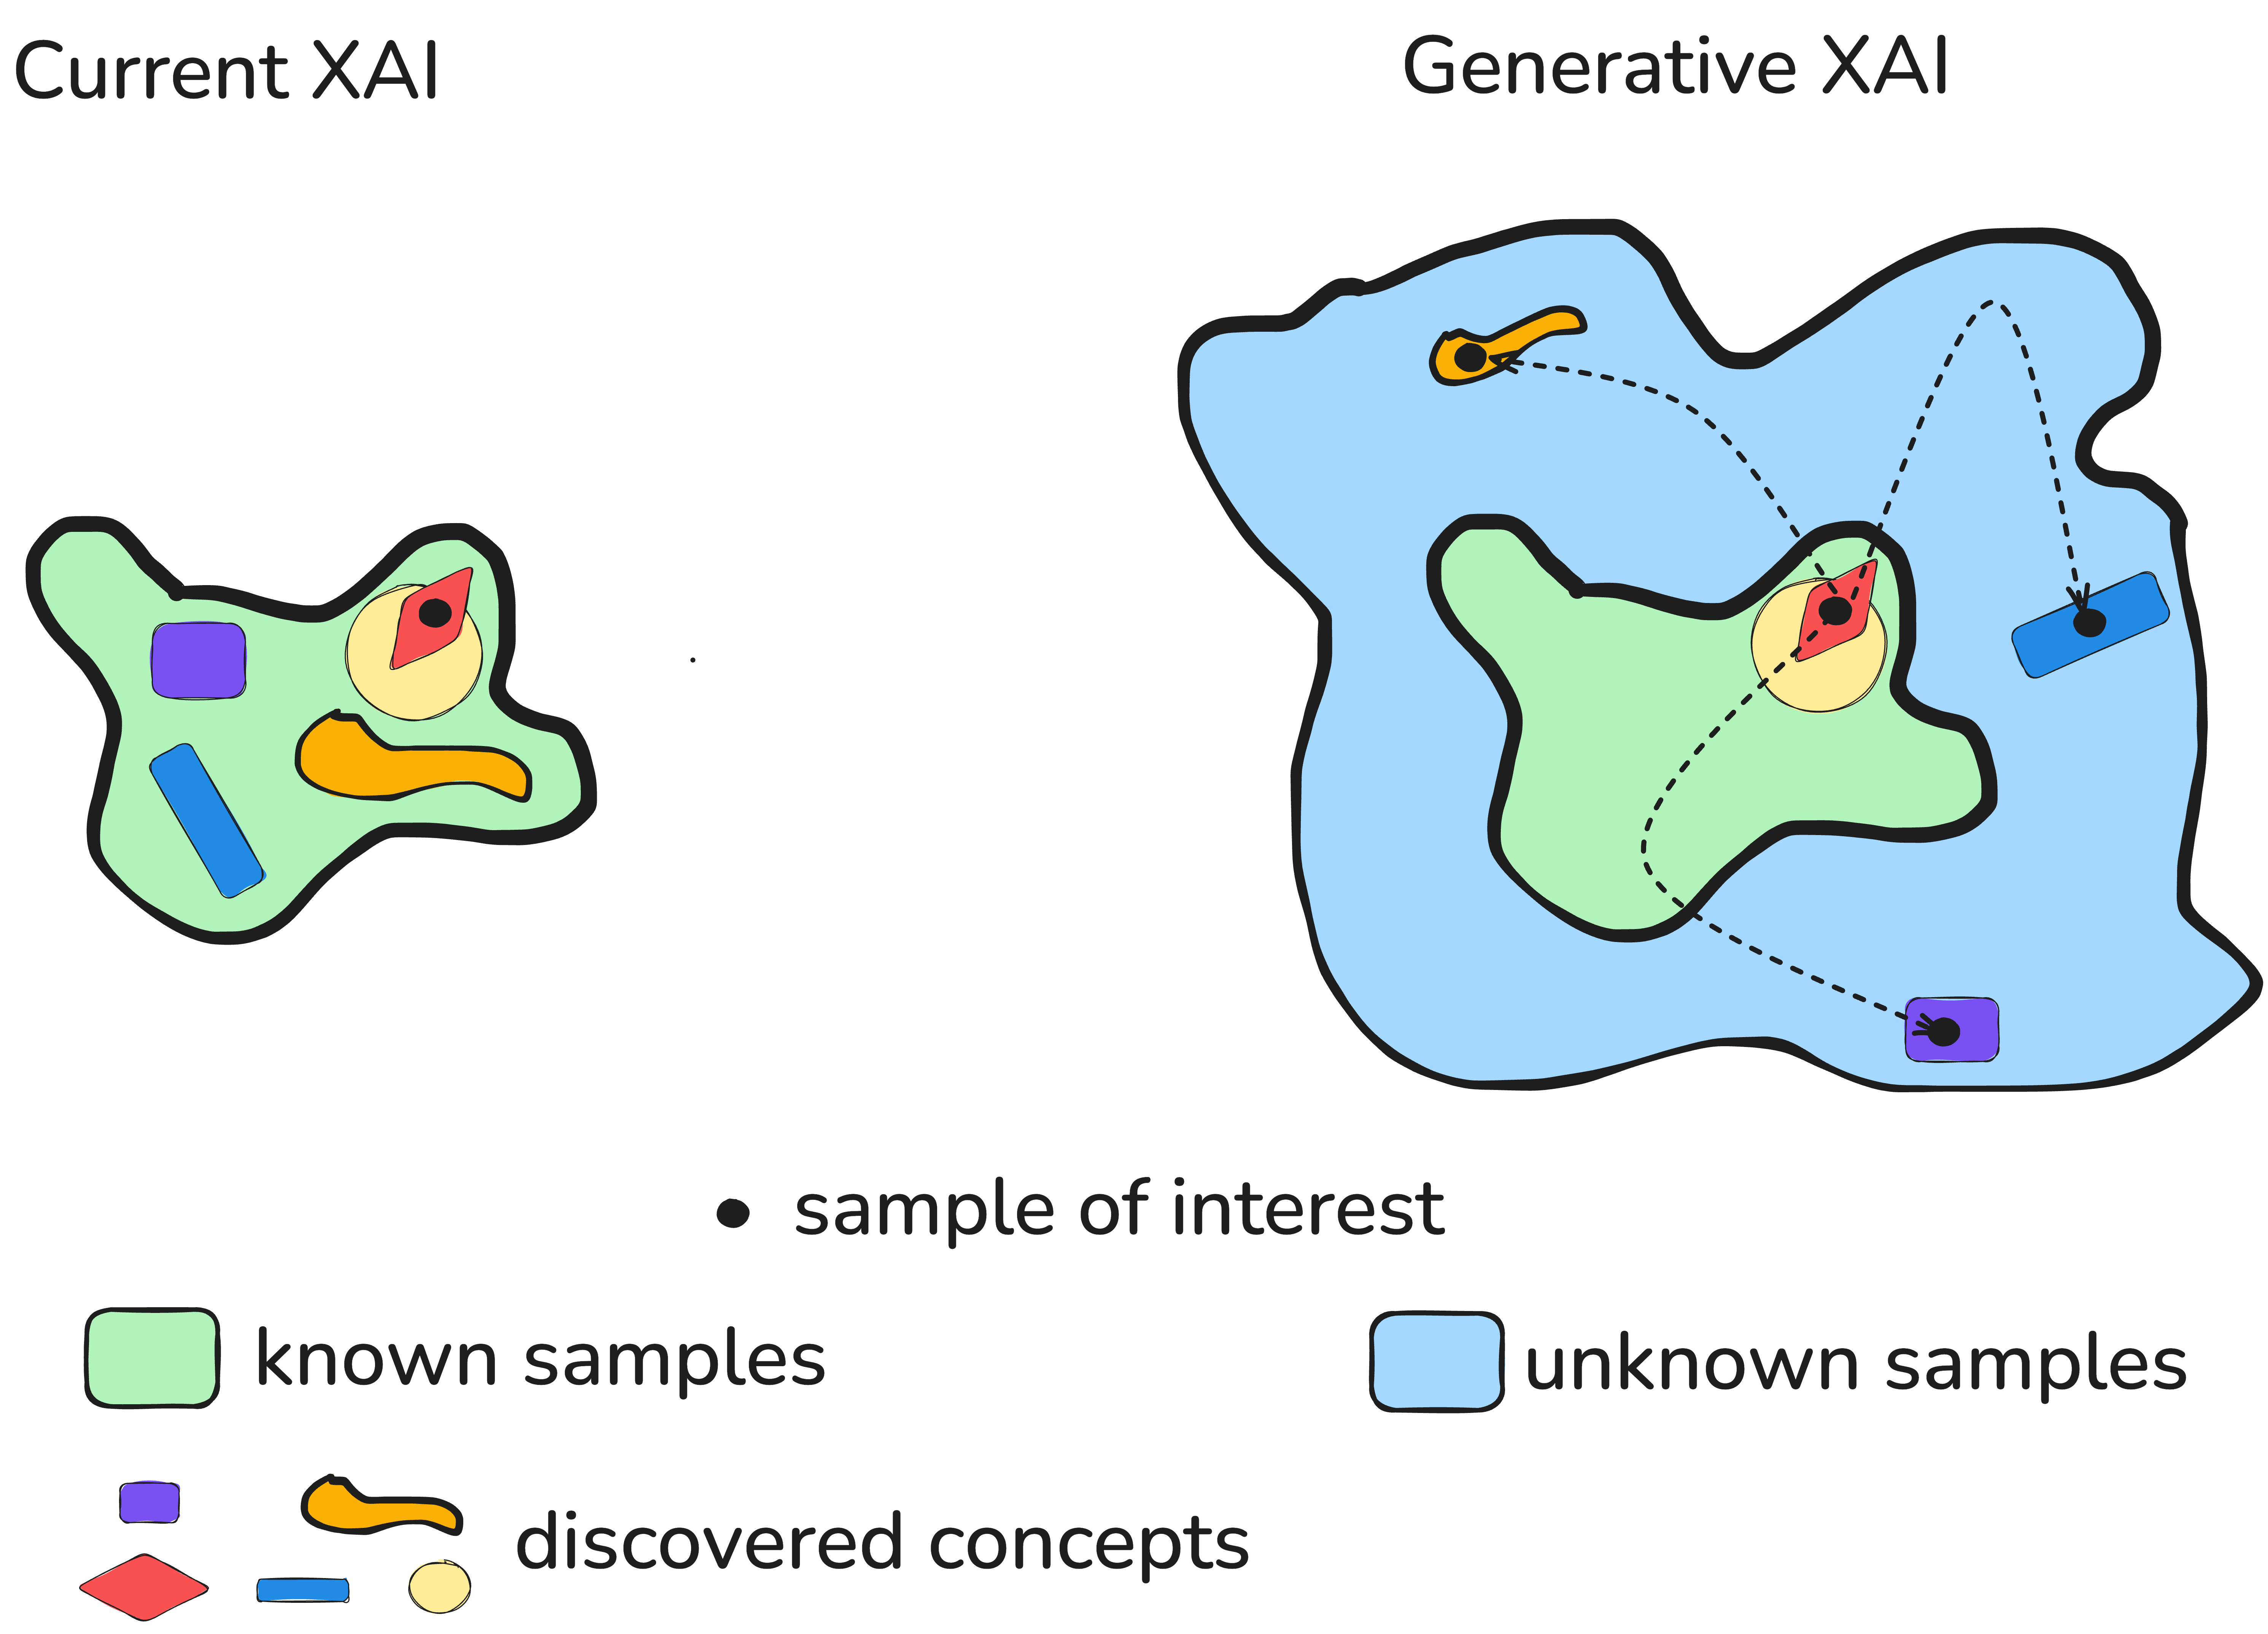
\includegraphics[width=0.8\linewidth]{figures/main/teaser1.png}
\caption{Conceptual comparison between traditional XAI methods and Generative XAI. Traditional methods analyze known data samples (left), while proposed approach synthesizes diverse examples from the invariant set that yield identical predictions (right).}
\label{fig:1_teaser}
\end{figure}

\section{Contributions}

This thesis makes three key contributions to the field of XAI, as outlined in the abstract and detailed in Chapter~\ref{r:method}:

The first contribution represents a \textbf{paradigm shift from traditional XAI methods} that analyze human-interpretable features in known data samples to generative XAI methods that synthesize new samples. This fundamental change in perspective allows for exploration of vast regions of the input manifold that remain unexplored by current approaches, providing a more comprehensive understanding of model behavior beyond the confines of training datasets.

The second contribution introduces a \textbf{novel theoretical backbone for generative XAI methods}. This framework provides formal mathematical definitions of invariant sets and establishes their properties as equivalence relations, offering a rigorous foundation for understanding and generating diverse examples that yield identical model predictions.

The third contribution presents an \textbf{efficient algorithmic implementation of this framework}. This method combines score-based diffusion models with guided sampling to generate high-quality, diverse examples from invariant sets, enabling practical application of the theoretical framework to real-world neural network analysis and interpretation.

These contributions are comprehensively detailed and evaluated in Chapter~\ref{r:method}, where both the theoretical foundations and empirical validation of proposed approach are presented.

\section{Thesis Organization}

The remainder of this thesis is structured to provide a comprehensive exploration of proposed generative XAI approach. Chapter~\ref{r:related_work} reviews the relevant literature across XAI methods, generative modeling, and diffusion models, establishing the theoretical foundation for this work. Chapter~\ref{r:method} presents core theoretical framework and details the \method{} algorithm, providing the mathematical foundation for invariant set generation and the practical implementation of proposed approach.

Chapter~\ref{r:experiments} presents a comprehensive experimental evaluation demonstrating the effectiveness of proposed method across multiple neural network analysis paradigms, from individual neuron activation to complete classifier output preservation. Chapter~\ref{r:conclusion} synthesizes contributions and their significance for the field of XAI. It also outlines future work and possible applications of this contribution.


\chapter{Related Work}\label{r:related_work}

This chapter reviews the relevant literature across several interconnected areas that form the foundation of this work. The chapter begins with an overview of explainable AI methods, followed by background on score-based generative models, conditional generation techniques, and related work on activation maximization and concept discovery.

\section{Explainable Artificial Intelligence}

The field of explainable AI has evolved rapidly in response to the growing complexity and opacity of modern deep learning models. As neural networks have grown from simple perceptrons to massive transformer architectures with billions of parameters, the need for interpretability has become increasingly critical for deployment in high-stakes domains such as healthcare, finance, and autonomous systems. The fundamental challenge lies in bridging the semantic gap between the mathematical operations performed by neural networks and human-understandable concepts. Current approaches to explainable AI can be broadly categorized into several paradigms, each with distinct methodological foundations and complementary strengths and limitations.

\subsection{Attribution Methods}

Attribution methods aim to identify which input features are most important for a model's prediction in a form of a heatmap. Gradient-based methods like Integrated Gradients \citep{sundararajan2017axiomaticattributiondeepnetworks} and GradCAM \citep{8237336} compute the gradient of the output with respect to input features to determine importance scores. While computationally efficient, these methods are limited to local explanations around specific data points and can be sensitive to model architecture and input preprocessing.

Perturbation-based methods such as LIME \citep{ribeiro2016whyitrustyou} and SHAP \citep{lundberg2017unifiedapproachinterpretingmodel} evaluate feature importance by measuring how predictions change when features are masked or altered. These methods provide more model-agnostic explanations but are computationally expensive and may not capture complex feature interactions.

\subsection{Concept-Based Methods}

Concept-based explainability methods attempt to understand models in terms of human-interpretable concepts. Concept Activation Vectors (CAVs) \citep{kim2018interpretabilityfeatureattributionquantitative} learn linear directions in activation space that correspond to human-defined concepts. Network Dissection \citep{bau2017networkdissectionquantifyinginterpretability} automatically discovers concepts by correlating individual neurons with semantic segmentation labels.

More recent work has focused on discovering concepts automatically without human supervision. ACE (Automatic Concept Extraction) \citep{ghorbani2019automaticconceptbasedexplanations} uses unsupervised segmentation to identify important concepts, while TCAV (Testing with CAVs) \citep{kim2018interpretabilityfeatureattributionquantitative} provides statistical significance testing for concept importance.

\subsection{Counterfactual Explanations}

Counterfactual explanations answer the question "What would need to change for the model to make a different prediction?" This paradigm has gained popularity due to its intuitive nature and practical utility. Although earlier work has explored generative models for visual counterfactual explanations, \citep{sobieski2024rethinkingvisualcounterfactualexplanations} advanced this direction in a way that directly inspired proposed approach. This method is, to best knowledge, the first to combine high-quality results with almost real-time performance.

In counterfactual methods, the objective is generally defined as finding the smallest possible changes to an input that alter the model’s decision—for example, modifying a few pixels in an image so that the predicted class changes. In contrast, the goal of this work is to generate diverse examples that preserve the original prediction.

\section{Score-Based Generative Models}\label{sec:sgm_background}

Score-based generative models (SGMs) have emerged as a powerful framework for high-quality image generation. Following the seminal work of \citep{song2021scorebasedgenerativemodelingstochastic}, these models can be understood through the lens of stochastic differential equations (SDEs).

\subsection{Mathematical Foundation}

The core idea behind SGMs is to transform samples from a complex data distribution $p_0$ (e.g. natural images) to a simple noise distribution $p_1$ (typically Gaussian) through a forward diffusion process and then learn to reverse this transformation. The forward SDE is given by:

\begin{equation}
\diff \mathbf{x}_t = \mathbf{f}(\mathbf{x}_t, t) \diff t + g(t) \diff \mathbf{w}_t
\label{eq:forward_sde}
\end{equation}

where $\mathbf{x}_t$ represents the noisy version of a clean image at time $t \in [0, 1]$, $\mathbf{f}(\mathbf{x}_t, t)$ is the drift coefficient, $g(t)$ is the diffusion coefficient, and $\mathbf{w}_t$ is a Wiener process.

The corresponding reverse SDE, which enables generation, is:

\begin{equation}
\diff \mathbf{x}_t = [\mathbf{f}(\mathbf{x}_t, t) - g(t)^2 \nabla_{\mathbf{x}_t} \log p_t(\mathbf{x}_t)] \diff t + g(t) \diff \bar{\mathbf{w}}_t
\label{eq:reverse_sde}
\end{equation}

The key term $\nabla_{\mathbf{x}_t} \log p_t(\mathbf{x}t)$ is the score function, which must be learned by a neural network $\mathbf{s}{\boldsymbol{\theta}}(\mathbf{x}_t, t)$, since it cannot be computed analytically without access to the final, fully denoised image.

\subsection{Training and Sampling}

Score networks are typically trained using denoising score matching \citep{6795935, song2020generativemodelingestimatinggradients}:

\begin{equation}
\mathcal{L}(\boldsymbol{\theta}) = \mathbb{E}_{t, \mathbf{x}_0, \boldsymbol{\epsilon}} \left[ \lambda(t) \|\mathbf{s}_{\boldsymbol{\theta}}(\mathbf{x}_t, t) - \boldsymbol{\epsilon}\|_2^2 \right]
\label{eq:score_matching_loss}
\end{equation}

where $\mathbf{x}_t = \alpha(t)\mathbf{x}_0 + \sigma(t)\boldsymbol{\epsilon}$ with $\boldsymbol{\epsilon} \sim \mathcal{N}(0, \mathbf{I})$, and $\lambda(t)$ is a weighting function.

During sampling, one starts from pure noise $\mathbf{x}_1 \sim \mathcal{N}(0, \mathbf{I})$ and integrate the reverse SDE using numerical solvers, with the learned score function $\mathbf{s}_{\boldsymbol{\theta}}$ approximating the true score.

\section{Conditional Generation and Classifier Guidance}

Conditional generation extends SGMs to produce samples conditioned on additional information $\mathbf{y}$, such as class labels or other attributes. To understand how conditioning works, one must first establish the mathematical foundation of score functions and their conditional decomposition.

\subsection{Score Function Fundamentals}

The score function $\nabla_{\mathbf{x}} \log p(\mathbf{x})$ represents the gradient of the log-probability density with respect to the input. In the context of diffusion models, the score function $\nabla_{\mathbf{x}_t} \log p_t(\mathbf{x}_t)$ provides the direction of steepest ascent in log-probability space at diffusion time $t$, essentially pointing toward regions of higher probability density. This geometric interpretation is crucial for understanding how diffusion models learn to reverse the noise process: by following the score function, one moves from low-probability noisy regions toward high-probability clean data regions.

The conditional score function $\nabla_{\mathbf{x}_t} \log p(\mathbf{x}_t \mid \mathbf{y}, t)$ extends this concept to conditional distributions, providing gradients that guide generation toward samples that satisfy the conditioning constraint $\mathbf{y}$. The key insight is that this conditional score can be decomposed using Bayes' theorem, allowing us to separate the unconditional generative component from the conditioning component.

\subsection{Conditional Score Decomposition}

Starting from Bayes' theorem for conditional probabilities:
$$p(\mathbf{x}_t \mid \mathbf{y}, t) = \frac{p(\mathbf{y} \mid \mathbf{x}_t, t) p(\mathbf{x}_t, t)}{p(\mathbf{y}, t)}$$

Taking the logarithm of both sides:
$$\log p(\mathbf{x}_t \mid \mathbf{y}, t) = \log p(\mathbf{y} \mid \mathbf{x}_t, t) + \log p(\mathbf{x}_t, t) - \log p(\mathbf{y}, t)$$

Since the marginal probability $p(\mathbf{y}, t)$ does not depend on $\mathbf{x}_t$, its gradient with respect to $\mathbf{x}_t$ is zero. Therefore, taking the gradient with respect to $\mathbf{x}_t$ yields the fundamental conditional score decomposition:

\begin{equation}
\nabla_{\mathbf{x}_t} \log p(\mathbf{x}_t \mid \mathbf{y}, t) = \nabla_{\mathbf{x}_t} \log p(\mathbf{x}_t, t) + \nabla_{\mathbf{x}_t} \log p(\mathbf{y} \mid \mathbf{x}_t, t)
\label{eq:conditional_score}
\end{equation}

\subsection{Classifier Guidance}

Classifier guidance \citep{dhariwal2021diffusionmodelsbeatgans} implements conditional generation by training an auxiliary time-dependent classifier $p_{\boldsymbol{\phi}}(\mathbf{y} \mid \mathbf{x}_t, t)$ on noisy images and incorporating its gradients into the sampling process:

\begin{equation}
\tilde{\mathbf{s}}_{\boldsymbol{\theta}}(\mathbf{x}_t, t, \mathbf{y}) = \mathbf{s}_{\boldsymbol{\theta}}(\mathbf{x}_t, t) + s \cdot \nabla_{\mathbf{x}_t} \log p_{\boldsymbol{\phi}}(\mathbf{y} \mid \mathbf{x}_t, t)
\label{eq:classifier_guidance}
\end{equation}

where $s$ is the guidance scale that controls the trade-off between sample quality and diversity.

\subsection{Limitations of Standard Classifier Guidance}

While effective for class-conditional generation, standard classifier guidance has several fundamental limitations that significantly impact its applicability to invariant set generation. These constraints arise from the architecture of diffusion models and the mathematical formulation of the guidance mechanism itself.

\textbf{Limited Optimization Horizon and Temporal Constraints:} The first major limitation stems from the inherently discrete and temporally constrained nature of the diffusion sampling process. Standard classifier guidance applies conditioning signals only at predetermined timesteps during the denoising trajectory, typically following a fixed schedule (e.g., every 10 steps out of 1000 total steps).

The mathematical consequence of this limitation becomes apparent when considering the precision requirements for other generations. While class-conditional generation can tolerate approximate conditioning (e.g., generating "roughly dog-like" images), it does not allow to iterating until some condition is meet, rather untill the schedule is finished. The discrete optimization steps available in classifier guidance provide insufficient granularity to achieve arbitraty high precision, particularly for complex objective functions with narrow convergence basins.

In practical applications, this limitation manifests as generated samples that approximate but do not precisely satisfy the given condition, leading to activation mismatches that can accumulate and compromise the interpretability of the results. For instance, when attempting to preserve specific neuron activations, the discrete guidance steps may succeed in maintaining the general semantic concept but fail to achieve the exact activation value.

\textbf{Latent Space Misalignment and Representational Incompatibility:} The second critical limitation arises from the architectural choice of modern diffusion models to operate in compressed latent spaces rather than directly in pixel space. This design, exemplified by Latent Diffusion Models (LDMs) \citep{rombach2022highresolutionimagesynthesislatent}, introduces a fundamental representational mismatch between the diffusion process and the neural networks being analyzed.

The mathematical formulation of this problem is subtle but profound. The diffusion model operates on encoded representations $\mathbf{z}_t = \mathcal{E}(\mathbf{x}_t)$ where $\mathcal{E}$ is a learned encoder (typically from a variational autoencoder), while the target neural network $f_{\boldsymbol{\theta}}$ operates on natural images $\mathbf{x}$. Classifier guidance requires evaluating $\nabla_{\mathbf{x}_t} \log p(\mathbf{y} \mid \mathbf{x}_t, t)$ at intermediate diffusion timesteps, but the noisy intermediate states $\mathbf{x}_t$ may not correspond to meaningful inputs for the classifier network.

This mismatch has several cascading consequences. First, training timestep-specific classifiers $p_{\boldsymbol{\phi}}(\mathbf{y} \mid \mathbf{x}_t, t)$ requires extensive additional data collection and training, essentially requiring a separate classifier for each timestep $t$. These classifiers must learn to operate on partially denoised, potentially unrealistic images, which significantly complicates the training process and may introduce systematic biases. Second, using approximate reconstructions $\hat{\mathbf{x}}_0(t)$ to evaluate the classifier introduces prediction errors that compound throughout the sampling process, potentially driving generation away from true invariant set membership.

The practical impact is particularly severe for fine-grained objectives like individual neuron activations or sparse autoencoder features, where small representational inconsistencies can have significan result on the final image. The latent space encoding may not preserve the specific visual patterns that activate particular neurons, leading to guidance signals that are misaligned with the true optimization objective.

\textbf{Objective Function Generalizability and Mathematical Constraints:} The third fundamental limitation concerns the restricted mathematical formulation of standard classifier guidance, which is specifically designed for classification objectives of the form $p(\mathbf{y} \mid \mathbf{x}_t, t)$ where $\mathbf{y}$ represents class labels or categorical conditions. This formulation, while elegant for its intended purpose, creates significant barriers when adapting to the diverse range of objective functions required for comprehensive neural network analysis.

The standard guidance formulation assumes that the conditioning variable $\mathbf{y}$ can be meaningfully interpreted as a class probability distribution, enabling the computation of log-probabilities and their gradients. However, one can require conditioning on arbitrary differentiable functions such as individual neuron activations (real-valued scalars), sparse autoencoder feature combinations (high-dimensional vectors), or complex geometric properties of the decision boundary (potentially non-linear manifolds in activation space).

Adapting classifier guidance to these objectives requires substantial mathematical reformulation, including the design of appropriate loss functions, normalization schemes, and gradient computation strategies. For example, when targeting a specific neuron activation value $a^*$, one must define a pseudo-probability distribution over activation values and ensure that the resulting gradients provide meaningful guidance signals. This often involves ad-hoc transformations like $p(a^* \mid \mathbf{x}_t, t) = \exp(-\lambda ||f_n(\mathbf{x}_t) - a^*||^2)$ where $\lambda$ is a temperature parameter that must be carefully tuned.

The consequences extend beyond mathematical complexity to fundamental questions of convergence and stability. The guidance gradients derived from these adapted objective functions may not exhibit the favorable convergence properties of the original classification formulation, potentially leading to unstable optimization dynamics, mode collapse, or failure to reach the target invariant set. Moreover, the interaction between multiple objectives (e.g., simultaneously constraining several neuron activations) becomes mathematically intractable within the standard guidance framework, limiting the approach to simple, single-objective scenarios.

These three limitations collectively demonstrate why standard classifier guidance, despite its success in class-conditional generation, has tsx fundamental limitations. This analysis directly motivates proposed infinite optimization approach, which addresses each of these constraints through decoupled optimization, native pixel-space operation, and arbitrary objective function support.

\section{Inverse Problems and Posterior Sampling}

Recent work has explored the use of diffusion models as priors for solving inverse problems in image restoration \citep{song2023pseudoinverse, chung2024diffusionposteriorsamplinggeneral}. The general inverse problem can be formulated as:

\begin{equation}
\mathbf{y} = \mathcal{A}(\mathbf{x}) + \boldsymbol{\epsilon}
\label{eq:inverse_problem}
\end{equation}

where $\mathcal{A}$ is a (possibly nonlinear) forward operator, $\mathbf{x}$ is the unknown signal, $\mathbf{y}$ is the observed measurement, and $\boldsymbol{\epsilon}$ is an additive noise term, which may follow different distributions (e.g., Gaussian, Poisson) and can exhibit nontrivial covariance structures.

\citep{chung2024diffusionposteriorsamplinggeneral} showed that diffusion models can address nonlinear inverse problems for arbitrary differentiable forward systems by incorporating the measurement likelihood into the reverse SDE. Their framework accommodates various noise models, including Gaussian and Poisson. This is particularly relevant to proposed approach, as neural network predictions can be interpreted as nonlinear measurements of the input image.

\subsection{Diverse Posterior Sampling}

More recently, \citep{cohen2024posteriorsamplingmeaningfuldiversity} extended inverse problem solvers to generate diverse solutions rather than a single best estimate. This paradigm shift from point estimation to posterior sampling aligns closely with proposed goal of generating new data samples.

\section{Activation Maximization and Feature Visualization}

Activation maximization techniques attempt to synthesize inputs that maximally activate specific neurons or model outputs \citep{erhan2009visualizing, mordvintsev2015deepdream}. The basic approach optimizes an input image $\mathbf{x}$ to maximize an objective function $\mathcal{L}(\mathbf{x})$:

\begin{equation}
\mathbf{x}^* = \arg\max_{\mathbf{x}} \mathcal{L}(\mathbf{x}) - \lambda \mathcal{R}(\mathbf{x})
\label{eq:activation_maximization}
\end{equation}

where $\mathcal{R}(\mathbf{x})$ is a regularization term that enforces constraints to encourage natural-looking images, and $\lambda$ controls the strength of regularization relative to the primary objective.

\subsection{The Critical Role of Regularization in Neural Visualization}

The regularization term $\mathcal{R}(\mathbf{x})$ represents one of the most fundamental challenges in neural network interpretability: ensuring that synthetic explanations reflect semantically meaningful patterns rather than exploiting imperceptible statistical quirks in the learned representations. Without appropriate regularization, activation maximization degenerates into adversarial optimization, producing images that achieve maximal neural activation through high-frequency noise patterns, texture irregularities, or other artifacts that are invisible to human perception but strongly trigger specific computational pathways.

The mathematical necessity for regularization arises from the high-dimensional nature of the optimization landscape. Neural networks, particularly deep convolutional architectures, exhibit complex response surfaces with numerous local maxima that correspond to spurious activation patterns. Without constraints, gradient-based optimization will exploit these pathways, leading to solutions that satisfy the mathematical objective while completely failing the interpretability goal. This fundamental tension between mathematical optimality and perceptual meaningfulness defines the core challenge of activation maximization.

\subsection{Classical Regularization Approaches}

Traditional regularization strategies for activation maximization fall into several categories, each addressing different aspects of the realism constraint:

\textbf{Total Variation Regularization:} The most commonly employed approach uses total variation (TV) penalties of the form $\mathcal{R}_{TV}(\mathbf{x}) = \sum_{i,j} |\mathbf{x}_{i+1,j} - \mathbf{x}_{i,j}| + |\mathbf{x}_{i,j+1} - \mathbf{x}_{i,j}|$, which encourages spatial smoothness by penalizing large gradients between adjacent pixels. While computationally efficient and mathematically well-defined, TV regularization often produces overly smoothed results that lack the fine-grained details characteristic of natural images, leading to blob-like visualizations that obscure important textural features.

\textbf{Frequency Domain Constraints:} Recognizing that natural images exhibit specific spectral characteristics, frequency-based regularization methods constrain the power distribution across spatial frequencies. These approaches typically apply band-pass filters or spectral penalties to encourage generated images to match the $1/f$ power law observed in natural image statistics. However, naive frequency constraints can be overly restrictive, suppressing legitimate high-frequency details while failing to address more subtle forms of adversarial exploitation.

\textbf{Statistical Prior Matching:} More sophisticated approaches attempt to match higher-order statistical properties of natural images, including local contrast distributions, edge orientation histograms, and texture statistics. These methods often involve complex optimization procedures and may require extensive parameter tuning, limiting their practical applicability while still failing to guarantee perceptual realism.

\subsection{Perceptual Metrics and Deep Regularization}

The limitations of classical approaches have motivated the development of perceptually-aware regularization methods that leverage learned representations of visual similarity:

\textbf{LPIPS (Learned Perceptual Image Patch Similarity):} The LPIPS metric \citep{zhang2018perceptual} represents a significant advancement in perceptual regularization, utilizing features from pre-trained neural networks (such as AlexNet or VGG \citep{krizhevsky2012imagenet,simonyan2014very}) to measure perceptual distance between images. Unlike pixel-based metrics that treat all spatial frequencies equally, LPIPS weights differences according to human perceptual sensitivity, providing a more meaningful measure of visual similarity. In the context of activation maximization, LPIPS can be incorporated as $\mathcal{R}_{LPIPS}(\mathbf{x}) = \text{LPIPS}(\mathbf{x}, \mathbf{x}_{natural})$ where $\mathbf{x}_{natural}$ represents a reference natural image or a distribution of natural images.

The mathematical formulation of LPIPS involves computing feature representations $\phi_l(\mathbf{x})$ at multiple layers $l$ of a pre-trained network, then measuring weighted $L_2$ distances: $\text{LPIPS}(\mathbf{x}, \mathbf{y}) = \sum_l w_l \|\phi_l(\mathbf{x}) - \phi_l(\mathbf{y})\|_2^2$ where $w_l$ are learned layer weights that reflect perceptual importance. This approach effectively uses one neural network to regularize the visualization of another, creating a hierarchical constraint system that can capture both low-level textural properties and high-level semantic consistency.

\textbf{Feature Distribution Matching:} Beyond pairwise similarity metrics, advanced regularization approaches constrain generated images to lie within the natural image manifold by matching statistical properties of deep feature distributions. These methods may employ techniques such as maximum mean discrepancy (MMD) or adversarial losses to ensure that synthetic visualizations exhibit feature statistics consistent with natural imagery across multiple representation levels \citep{goodfellow2014generative, dziugaite2015traininggenerativeneuralnetworks}.

\textbf{Gram Matrix Constraints:} Inspired by neural style transfer, some approaches regularize activation maximization using Gram matrix constraints that preserve spatial correlations between feature maps while allowing optimization of the primary objective. This approach can maintain textural coherence while permitting the emergence of activation-specific patterns \citep{gatys2016image}.

\subsection{The Fundamental Challenge of Realistic Generation}

Despite these advances, generating truly realistic images through activation maximization remains an outstanding challenge with profound implications for explainable AI. The core difficulty lies in the fundamental mismatch between the objectives of neural networks (optimized for task performance) and the constraints of natural image generation (governed by complex physical and perceptual processes).

Neural networks, particularly those trained on large-scale datasets, develop internal representations that capture statistical regularities in training data but may not respect the underlying generative processes that produce natural images. When activation maximization attempts to reverse-engineer these representations, it encounters the problem that multiple distinct natural phenomena may activate the same neural pathway, while the optimization process tends to find the most mathematically efficient (often unrealistic) combination of these activating features.

This tension is particularly acute for neurons with complex, multi-faceted selectivity patterns. For instance, a neuron that responds to both curved edges and specific texture patterns may be maximally activated by an image containing impossible combinations of these features—curved edges with unnatural texture properties that could not exist in real objects. Traditional regularization approaches struggle to eliminate such impossible combinations while preserving the legitimate activation patterns that make the visualization interpretable.

The implications extend beyond individual visualization quality to the broader epistemological foundations of neural network interpretability. If our primary tools for understanding neural representations systematically produce unrealistic explanations, we risk developing misleading intuitions about how these systems actually process natural inputs. This represents the central challenge of non-adversarial explainability: developing interpretation methods that reveal genuine computational strategies rather than artifacts of the interpretation process itself.

Furthermore, the computational expense of sophisticated regularization approaches often makes them impractical for large-scale analysis, creating a trade-off between visualization quality and analytical scope. This limitation has motivated interest in alternative approaches, such as proposed diffusion-based method, that can leverage powerful generative priors to ensure realism while maintaining computational tractability.

\subsection{Limitations and Relationship to this Work}

Although activation maximization shares the goal of understanding model behavior through synthetic inputs, it differs fundamentally from proposed approach in ways that reveal critical limitations of single-sample interpretation methods and highlight the necessity of diverse, multi-sample analysis for comprehensive neural network understanding.

\textbf{The Diversity Imperative: Why Single Solutions Fail to Capture Neural Complexity}

The most fundamental limitation of traditional activation maximization lies in its pursuit of a single optimal solution rather than exploring the diverse space of inputs that activate neural pathways. This single-solution paradigm represents a profound philosophical and methodological constraint that severely limits our understanding of neural network decision-making processes.

Neural networks, particularly deep architectures trained on complex visual tasks, develop representations that are inherently multi-faceted and compositional. A single neuron may respond to diverse combinations of visual features: edges at specific orientations, particular color combinations, textural patterns, or higher-order statistical regularities in image structure. When activation maximization converges to a single "optimal" stimulus, it provides only one possible interpretation of this complex feature space, potentially missing equally valid—and often more interpretable—alternative patterns that achieve the same level of activation.

This limitation becomes particularly pronounced when we consider the high-dimensional nature of neural activation landscapes. The optimization surface for maximizing neuron activation typically contains multiple local maxima, each corresponding to different ways the neuron can be activated. Traditional optimization methods, constrained by computational budgets and convergence criteria, tend to settle into the first sufficiently strong local maximum encountered, never exploring the broader topology of activation-triggering patterns.

The diversity of activation patterns is not merely a technical curiosity but provides critical insights into the robustness, generalization, and potential failure modes of neural networks. Consider a hypothetical neuron that achieves maximal activation through three distinct pathways: geometric patterns with high contrast edges, specific color combinations under particular lighting conditions, and textural regularities found in biological surfaces. A single-solution activation maximization approach might converge to only one of these patterns—perhaps the highest-contrast geometric configuration—leaving the other two activation modes completely unexplored and potentially unrecognized.

From a scientific interpretability perspective, this represents a fundamental sampling bias in our understanding of neural representations. If our primary tool for neural interpretation systematically undersamples the space of activating patterns, we develop incomplete and potentially misleading theories about what these networks have learned. This is particularly problematic for safety-critical applications where understanding the full range of inputs that can trigger specific network behaviors is essential for identifying potential failure modes or adversarial vulnerabilities.

\textbf{Maximum Activation vs. Preserved Predictions: Methodological Paradigm Differences}

The second critical difference lies in the optimization objectives themselves. Activation maximization seeks to find inputs that produce maximum possible activation: $\mathbf{x}^* = \arg\max_{\mathbf{x}} \mathcal{L}(\mathbf{x})$, where the goal is to push the neuron's response as high as possible. This approach, while providing insights into the extreme cases of neural activation, may not reflect the typical operational range of the neuron during normal inference on natural images.

In contrast, proposed invariant set approach preserves specific prediction values: $\mathcal{L}(\mathbf{x}) = \mathcal{L}(\mathbf{x^*})$, where we maintain the exact activation level observed for a reference input. This distinction is not merely technical but reflects fundamentally different philosophical approaches to neural interpretation. Maximum activation reveals the theoretical limits of neural responsiveness but may correspond to unrealistic or pathological input configurations that never occur in practice. Preserved predictions, however, explore the manifold of realistic inputs that produce the same computational outcome, providing insights into the equivalence classes that define the network's decision boundaries.

This difference has profound implications for understanding model robustness and generalization. Maximum activation methods may reveal activation patterns that, while mathematically optimal, represent adversarial or out-of-distribution inputs that provide limited insight into normal model operation. Preserved prediction methods, by maintaining activation levels within the natural range observed during typical inference, ensure that generated explanations remain grounded in the model's operational reality.

Furthermore, the preserved prediction paradigm enables more sophisticated analyses of neural network decision-making. By generating diverse samples that maintain identical predictions, we can study the invariance properties of neural representations, identify the minimal sets of features necessary for specific classifications, and understand how different visual patterns can be considered equivalent by the network. This level of analysis is impossible with traditional activation maximization, which focuses solely on the extreme points of the activation landscape.

\textbf{Quality and Realism: The Adversarial Explanation Problem}

The third fundamental limitation concerns the quality and realism of generated explanations. Traditional activation maximization methods, despite sophisticated regularization approaches, continue to produce explanations that often appear unnatural or adversarial. These images may contain high-frequency artifacts, impossible geometric configurations, or other visual anomalies that, while effectively activating target neurons, provide misleading insights into how these networks process natural images.

This "adversarial explanation" problem extends beyond mere aesthetic concerns to fundamental questions about the validity and trustworthiness of neural network interpretations. If our primary tools for understanding neural representations systematically produce unrealistic explanations, we risk developing intuitions about neural network behavior that are fundamentally divorced from how these systems actually operate on natural inputs.

The prevalence of unrealistic patterns in activation maximization results suggests that many neurons exhibit complex multi-modal activation landscapes where the global maximum corresponds to artificial or pathological input configurations rather than meaningful natural patterns. This phenomenon indicates that the traditional approach of seeking maximum activation may be fundamentally misaligned with the goal of understanding natural neural responses.

Our diffusion-based approach addresses this limitation by leveraging powerful generative priors that ensure generated samples remain within the natural image manifold. By constraining the optimization process to operate within the space of realistic images—as defined by the training distribution of a high-quality diffusion model—we ensure that all generated explanations correspond to plausible visual inputs. This constraint fundamentally changes the nature of the optimization problem, shifting focus from mathematical extremes to realistic variations within the natural image distribution.

The implications of this constraint extend beyond image quality to the epistemological foundations of neural network interpretability. By ensuring that all generated explanations correspond to realistic inputs, we can be confident that our insights into neural network behavior reflect genuine computational strategies rather than artifacts of the interpretation method. This paradigm shift from adversarial optimization to realistic generation represents a fundamental advance in the reliability and trustworthiness of neural network explanations.

Moreover, the diversity enabled by proposed approach provides a more comprehensive view of neural network decision-making that captures the full range of natural variations that can produce identical network responses. This diversity is not merely quantitative—generating more examples—but qualitative, revealing fundamentally different types of visual patterns that achieve the same computational outcome and providing insights into the flexibility and robustness of learned neural representations.

\subsection{Examples of Unrealistic Activation Maximization Results}

To illustrate the fundamental problems with traditional activation maximization approaches, it is instructive to examine specific examples of the unrealistic images these methods typically produce. These examples demonstrate why the interpretability community has increasingly recognized the need for alternative approaches that ensure visual realism.

\textbf{High-Frequency Noise Patterns:} One of the most common failure modes of activation maximization involves the generation of images dominated by high-frequency noise that appears as television static or random pixel patterns to human observers. For instance, \citet{olah2017feature} documented cases where activation maximization for individual neurons in AlexNet produced images consisting almost entirely of checkerboard patterns, diagonal stripes, or seemingly random high-contrast pixels arranged in regular grids. While these patterns achieve maximal activation for their target neurons—sometimes reaching activation levels 10-100 times higher than typical natural images—they provide no meaningful insight into what visual concepts the neurons have learned to detect in realistic scenarios.

The mathematical reason for this phenomenon lies in the optimization dynamics: high-frequency patterns can create large gradient magnitudes that drive rapid increases in activation, even when such patterns never occur in natural imagery. A neuron that responds strongly to edge-like features, for example, may be maximally activated by an image containing impossible combinations of edges at every pixel location, creating a visually incoherent pattern that exploits the mathematical structure of the learned filter without respecting the constraints of natural image formation.

\textbf{Impossible Geometric Configurations:} Another category of unrealistic activation maximization results involves geometrically impossible objects or spatial arrangements that could not exist in three-dimensional space. \citet{szegedy2014goingdeeperconvolutions} and subsequent work have documented numerous examples where neurons supposedly detecting "car wheels" produce circular patterns that appear simultaneously at multiple depths, violate perspective geometry, or exhibit lighting conditions that are physically impossible.

Consider a hypothetical neuron trained to detect car wheels in natural images. Activation maximization might produce an image containing dozens of wheel-like circular patterns scattered across the image plane, each with different apparent sizes and orientations that collectively create a visually incoherent scene. While each individual circular pattern might resemble a wheel when viewed in isolation, the overall spatial arrangement violates basic principles of perspective, occlusion, and lighting consistency that govern real-world imagery. Such results provide misleading insights about the neuron's true selectivity, suggesting it detects "wheels" when it may actually respond to simpler geometric regularities like circular edges or radial symmetries.

\textbf{Textural Impossibilities and Material Inconsistencies:} A particularly problematic category involves the generation of surface textures or material properties that cannot exist in nature. Activation maximization for neurons supposedly selective for animal fur, for example, might produce images where fur-like textures transition abruptly into metallic surfaces, or where organic textures exhibit perfect mathematical regularities that would be impossible to achieve through biological processes.

\citet{nguyen2016synthesizingpreferredinputsneurons} documented cases where activation maximization for a "dog face" classifier produced images containing dog-like features (ears, nose shape, eye placement) but with impossible material properties—metallic fur, geometrically perfect symmetries, or color patterns that violate the physical constraints of biological pigmentation. While these images successfully activate the target classifier with high confidence scores, they provide fundamentally misleading information about the visual features that constitute "dog-ness" in natural contexts.

\textbf{Scale and Perspective Violations:} Traditional activation maximization often produces images where objects appear at impossible scales or with inconsistent perspective cues. A neuron trained on natural images of buildings might be maximally activated by an image containing architectural elements that simultaneously appear both extremely close (based on texture detail) and extremely distant (based on perspective cues), creating a visual impossibility that exploits multiple activation pathways simultaneously.

\textbf{Adversarial Feature Combinations:} Perhaps most problematically, activation maximization frequently combines legitimate visual features in adversarial ways that achieve mathematical optimality while completely destroying semantic coherence. For instance, a neuron that responds to both facial features and curved edges might be maximally activated by an image containing eye-like patterns arranged in geometric grids across curved surfaces, creating a result that simultaneously contains recognizable visual elements while forming an incomprehensible whole.

These examples illustrate why the traditional approach of seeking maximum activation is fundamentally misaligned with the goal of understanding how neural networks process natural imagery. The optimization process systematically favors mathematical efficiency over perceptual realism, leading to explanations that may be mathematically correct but provide misleading insights into the genuine computational strategies employed by the network during normal operation.

The prevalence and consistency of such unrealistic results across different architectures, datasets, and optimization procedures suggests that this is not merely a technical limitation that can be solved through better regularization, but rather a fundamental problem with the activation maximization paradigm itself. This recognition has motivated the development of alternative approaches, including proposed diffusion-based method, that prioritize realistic generation while maintaining mathematical rigor in preserving neural activation patterns.

\textbf{Crucially, even these most recent advances still stop short of producing images that resemble natural data.} As \citet{zhu2025representationunderstandingactivationmaximization} emphasize, pixel-space optimization remains dominated by noisy high-frequency artifacts, while frequency-domain methods—though smoother—frequently yield abstract textures or diffuse motifs that lack coherent object-level structure. The authors explicitly note that bridging the semantic gap between optimized patterns and human-recognizable concepts remains unresolved, underscoring that AM, despite incremental refinements, continues to fall short of generating realistic images

\section{Concept Discovery and Spurious Feature Detection}

Understanding what concepts neural networks learn has been an active area of research. \citep{Lapuschkin_2019} developed SpRAy, an automatic pipeline for exploring shortcuts and biases learned by models, often referred to as "Clever Hans" effects \citep{pfungst1911cleverHans}. \citet{neuhaus2023spuriousfeatureslargescale} investigates methods for automatically finding spurious features in training data.

Recent work by \citet{dreyer2025mechanisticunderstandingvalidationlarge} addresses the question of what concepts were learned by models and where in the training data they were present. However, \citep{leask2025sparse} argues that automatically discovered concepts may lack atomicity and completeness.

This work complements this line of research by exploring the space of inputs that preserve predictions, potentially revealing spurious correlations and biases that may not be apparent from training data analysis alone.

\section{Realistic Image Generation and Natural Image Statistics}

The fundamental challenge in generative neural network interpretability extends beyond producing mathematically correct results to ensuring that generated explanations appear realistic and semantically meaningful to human observers. This requirement for realism is not merely aesthetic but represents a critical methodological constraint that ensures the validity and trustworthiness of interpretability insights.

\subsection{Natural Image Statistics and Perceptual Realism}

Natural images exhibit specific statistical regularities that distinguish them from artificial or adversarial patterns. These regularities, developed through millions of years of evolution in biological vision systems and refined through decades of computer vision research, provide objective criteria for evaluating the realism of generated images.

The most fundamental characteristic of natural images is their power spectral density, which typically follows a $1/f^2$ power law across spatial frequencies \citep{field1987relations}. This spectral signature reflects the hierarchical structure of natural scenes, where large-scale geometric arrangements (buildings, horizons, object boundaries) contribute low-frequency components, while fine-grained details (textures, edges, surface patterns) contribute higher frequencies. Deviations from this spectral profile often indicate artificial generation or adversarial manipulation.

Beyond spectral properties, natural images exhibit specific statistical dependencies between neighboring pixels, consistent edge orientation distributions, and characteristic amplitude distributions in wavelet decompositions. These properties emerge from the physical processes that generate natural scenes—lighting conditions, surface materials, atmospheric scattering, and optical properties of imaging systems—and provide robust signatures for distinguishing realistic from artificial imagery.

\subsection{The Realism Imperative in Explainable AI}

For explainable AI applications, the requirement for realistic generation transcends technical considerations to address fundamental epistemological questions about the validity of synthetic explanations. If interpretation methods systematically produce unrealistic visualizations, they risk providing misleading insights about how neural networks process natural inputs.

Consider the implications of unrealistic explanations for different stakeholders: researchers developing new architectures may draw incorrect conclusions about feature learning if their analysis tools produce artificial patterns; practitioners deploying models in safety-critical applications may develop false confidence if explanations appear to show reasonable behavior on unrealistic inputs; and users of AI systems may lose trust if explanations appear divorced from recognizable visual concepts.

The realism constraint serves as a crucial validity check that ensures generated explanations remain grounded in the visual world that neural networks are designed to understand. By constraining interpretation methods to produce realistic images, this work ensures that insights reflect genuine computational strategies rather than artifacts of the interpretation process itself.

\subsection{Approaches to Ensuring Visual Realism}

Several methodological approaches have been developed to ensure that generated images maintain realistic appearance while satisfying specific mathematical constraints:

\textbf{Statistical Prior Matching:} Traditional approaches enforce realism by matching statistical properties of generated images to those observed in natural image datasets. This includes constraining first-order statistics (mean, variance), second-order statistics (spatial correlations), and higher-order regularities (edge orientation histograms, local contrast distributions). While computationally tractable, these approaches often fail to capture the complex, high-dimensional dependencies that characterize natural imagery.

\textbf{Learned Perceptual Metrics:} More sophisticated approaches utilize deep neural networks trained on large-scale image datasets to define perceptual similarity metrics. The LPIPS (Learned Perceptual Image Patch Similarity) metric, for example, leverages features from pre-trained networks to measure perceptual distance between images, providing a more nuanced assessment of visual realism than pixel-based metrics.

\textbf{Generative Model Priors:} The most powerful approach to ensuring realism involves leveraging the implicit priors learned by high-quality generative models. Diffusion models, GANs, and other deep generative architectures learn complex, high-dimensional probability distributions that capture the statistical structure of natural images. By constraining optimization to operate within the manifold defined by these learned distributions, we can ensure that generated images satisfy the complex dependencies that characterize realistic imagery.

\subsection{Frequency Domain Considerations}

Understanding the frequency domain characteristics of realistic images provides crucial insights for designing generation methods that produce perceptually meaningful results. Natural images typically concentrate most of their energy in low-to-mid frequency bands, with high-frequency content dominated by texture details and noise rather than semantic information.

This frequency distribution has important implications for interpretability methods. Adversarial optimization approaches often exploit high-frequency artifacts that are imperceptible to human observers but strongly activate neural network pathways. By analyzing the frequency content of generated explanations and ensuring consistency with natural image statistics, we can identify and eliminate such artifacts.

Proposed approach addresses this challenge through frequency-aware optimization that constrains generated images to exhibit spectral properties consistent with natural imagery. This ensures that invariant set membership is achieved through semantically meaningful variations rather than imperceptible high-frequency manipulation, providing explanations that reflect genuine visual concepts rather than mathematical artifacts.

\subsection{Perceptual Validation and Human-Centered Evaluation}

The ultimate test of realistic generation lies in human perceptual validation. While statistical metrics and learned similarity measures provide objective criteria for realism, human judgment remains the gold standard for evaluating whether generated images appear natural and semantically coherent.

This suggests the importance of incorporating human-centered evaluation into the development and validation of interpretability methods. Such evaluation can identify systematic biases or artifacts that may not be captured by automated metrics, ensuring that generated explanations provide meaningful insights for human users.

The integration of realistic generation constraints with precise mathematical objectives represents a fundamental advancement in interpretability methodology, ensuring that synthetic explanations remain grounded in the visual world while satisfying the rigorous requirements of scientific analysis.

\section{Conclusion and Synthesis}

After comprehensive analysis of the explainable AI landscape, several fundamental conclusions emerge about the current state of the field and the limitations that constrain progress toward truly comprehensive neural network interpretability.

\subsection{Synthesis of Current Approaches}

The evolution of explainable AI has progressed through distinct methodological paradigms, each addressing specific aspects of neural network interpretability while introducing new limitations. Attribution methods, from gradient-based approaches like Integrated Gradients to perturbation-based techniques like LIME and SHAP, have provided valuable insights into local feature importance but remain fundamentally constrained to analyzing existing data points and their immediate neighborhoods. These methods excel at answering "why did the model make this specific prediction?" but cannot address the broader question of "what other inputs would yield the same prediction?"

Concept-based methods have advanced our understanding by identifying human-interpretable patterns in neural representations, with frameworks like CAVs and Network Dissection revealing semantic structures within learned features. However, these approaches remain anchored to the statistical regularities present in training datasets, potentially missing conceptual relationships that extend beyond observed data distributions. The automatic concept discovery methods, while promising, still operate within the bounds of training data manifolds and may miss important invariance relationships that exist in unexplored regions of the input space.

Counterfactual explanation methods represent a significant conceptual advance by generating synthetic examples that alter model predictions, but they remain focused on boundary analysis rather than comprehensive exploration of decision-invariant regions. The emphasis on minimal perturbations, while valuable for understanding decision boundaries, limits the scope of insights that can be gained about the broader equivalence classes that define model behavior.

Score-based generative models and posterior sampling techniques have demonstrated remarkable capabilities in generating high-quality synthetic data, yet their application to neural network interpretability has been limited by the constraints of standard conditioning approaches. Classifier guidance, while effective for categorical conditioning, proves inadequate for the precise, continuous optimization required for invariant set exploration.

\subsection{Critical Limitations of Current Paradigms}

The analysis reveals several critical limitations that collectively constrain the field's ability to achieve comprehensive neural network interpretability:

\textbf{Data Distribution Constraint:} Perhaps most fundamentally, current XAI methods are inherently limited by their reliance on observed training data and its immediate statistical neighborhood. This constraint means that vast regions of the input manifold—regions that may contain crucial insights about model behavior, failure modes, and invariance properties—remain completely unexplored. The consequence is a systematically incomplete understanding of neural network decision-making that may miss critical behaviors not represented in training datasets.

\textbf{Single-Sample Interpretation Bias:} Traditional activation maximization and feature visualization approaches suffer from a fundamental single-solution bias that provides only partial insights into the complex, multi-faceted nature of neural representations. By converging to individual "optimal" examples, these methods miss the diversity of patterns that can activate identical computational pathways, leading to incomplete and potentially misleading interpretations of learned features.

\textbf{Adversarial Explanation Problem:} The persistent generation of unrealistic, artifact-laden explanations by optimization-based methods represents more than a technical limitation—it reflects a fundamental mismatch between mathematical optimization objectives and the constraints of natural image formation. This problem undermines the trustworthiness and applicability of interpretability insights, potentially leading to false conclusions about neural network behavior.

\textbf{Limited Semantic Scope:} Current methods typically reveal only narrow aspects of neural representations, missing the broader semantic relationships and invariance properties that define comprehensive model understanding. The focus on individual features or local perturbations fails to capture the global structure of learned representations and their relationships to natural data variations.

\subsection{What the Field Lacks}

After analysis of these diverse approaches and their limitations, the conclusion is that the field fundamentally lacks a unified framework for comprehensive exploration of neural network decision spaces beyond the constraints of observed training data. Specifically, current explainable AI research lacks:

\textbf{Generative Exploration Capabilities:} The field lacks methods that can systematically explore the space of alternative inputs yielding identical predictions while maintaining realistic visual appearance. This limitation prevents comprehensive understanding of model invariance properties and equivalence classes that define decision-making behavior.

\textbf{Invariance Set Analysis:} Current approaches lack the theoretical and methodological foundations for systematically analyzing the complete manifold of inputs that produce identical model outputs. Without this capability, interpretability remains fundamentally incomplete, missing crucial insights about model robustness, generalization, and potential failure modes.

\textbf{Multi-Scale Interpretability Integration:} The field lacks unified approaches that can simultaneously address interpretability at multiple scales—from individual neurons to complete model outputs—within a single coherent framework. This limitation fragments understanding and prevents development of comprehensive theories of neural network behavior.

\textbf{Realistic Constraint Satisfaction:} Perhaps most critically, the field lacks methods that can satisfy precise mathematical constraints (such as exact activation preservation) while ensuring generated explanations remain within the natural image manifold. This fundamental capability is essential for trustworthy interpretability that reflects genuine model behavior rather than mathematical artifacts.

\textbf{Diverse Posterior Sampling for Interpretability:} Finally, the field lacks the conceptual and methodological frameworks for treating neural network interpretability as a posterior sampling problem, where the goal is to generate diverse, representative samples from the space of inputs that satisfy specific behavioral constraints. This paradigm shift from point estimation to distributional analysis represents a crucial missing component in current interpretability research.

These deficiencies collectively constrain the field's ability to develop comprehensive, trustworthy, and practically applicable methods for understanding neural network decision-making processes. Addressing these limitations requires fundamental advances in both theoretical foundations and methodological approaches, motivating the generative framework presented in this thesis.


\chapter{EquiDiff: Equivariant Diffusion Sampling for Invariant Set Generation}\label{r:method}

This chapter presents the theoretical foundation and algorithmic details of our proposed approach for generating invariant sets of neural network representations. We begin with formal mathematical definitions, establish the relationship to classical level sets from differential topology \citep{lee2013smooth,milnor1965topology,fort2017gaussian}, detail our core algorithm, and conclude with implementation specifics and quality assurance measures.

\section{Theoretical Foundation and Formal Definitions}

We begin by establishing the mathematical foundations for our approach through formal definitions that clarify the key concepts and their relationships.

\begin{defi}[Invariant Framework]\label{def:invariants_framework}
Let $f: \mathbb{R}^n \rightarrow \mathbb{R}^m$ be a neural network with $n$ input dimensions and $m$ output dimensions, where $n$ represents the dimensionality of the input space (e.g., $n = W \times H \times C$ for images of width $W$, height $H$, and $C$ channels) and $m$ represents the dimensionality of the network component we wish to analyze (e.g., $m = 1$ for a single neuron, $m = k$ for $k$ class logits). The network $f$ can be viewed as a composition of functions $f = f_L \circ f_{L-1} \circ \ldots \circ f_1$, where each $f_i$ represents a layer transformation.

For a given query point $\mathbf{x}^* \in \mathbb{R}^n$, the \textbf{Invariant Framework} defines the theoretical foundation for identifying all inputs that produce identical network responses under a specified objective function.
\end{defi}

\begin{defi}[EquiDiff Method]\label{def:equidiff_method}
Given the Invariant Framework (Definition \ref{def:invariants_framework}), we define the \textbf{EquiDiff method} as an algorithmic approach that combines score-based diffusion models with infinite optimization to generate diverse, realistic samples from invariant sets.

Specifically, for a neural network $f: \mathbb{R}^n \rightarrow \mathbb{R}^m$ and query point $\mathbf{x}^*$, EquiDiff generates samples $\{\mathbf{x}_i\}_{i=1}^N$ through three integrated mechanisms. The method maintains an invariance constraint by ensuring $\|f(\mathbf{x}_i) - f(\mathbf{x}^*)\|_2 < \epsilon$ for small $\epsilon > 0$, where the $L_2$ distance between network outputs remains below a specified threshold. Simultaneously, a realism constraint ensures that generated samples $\mathbf{x}_i$ lie within the natural image manifold as defined by a pre-trained diffusion model, preventing the generation of adversarial artifacts or unrealistic patterns. Finally, a diversity constraint promotes semantic and visual variety among generated samples while preserving the strict invariance requirement, enabling exploration of the full breadth of patterns that activate identical network responses.

The method operates through infinite optimization over the latent space of a diffusion model, enabling precise control over network activations while ensuring realistic image generation through the inherent properties of the diffusion sampling process.
\end{defi}

\begin{figure}[h]
\centering
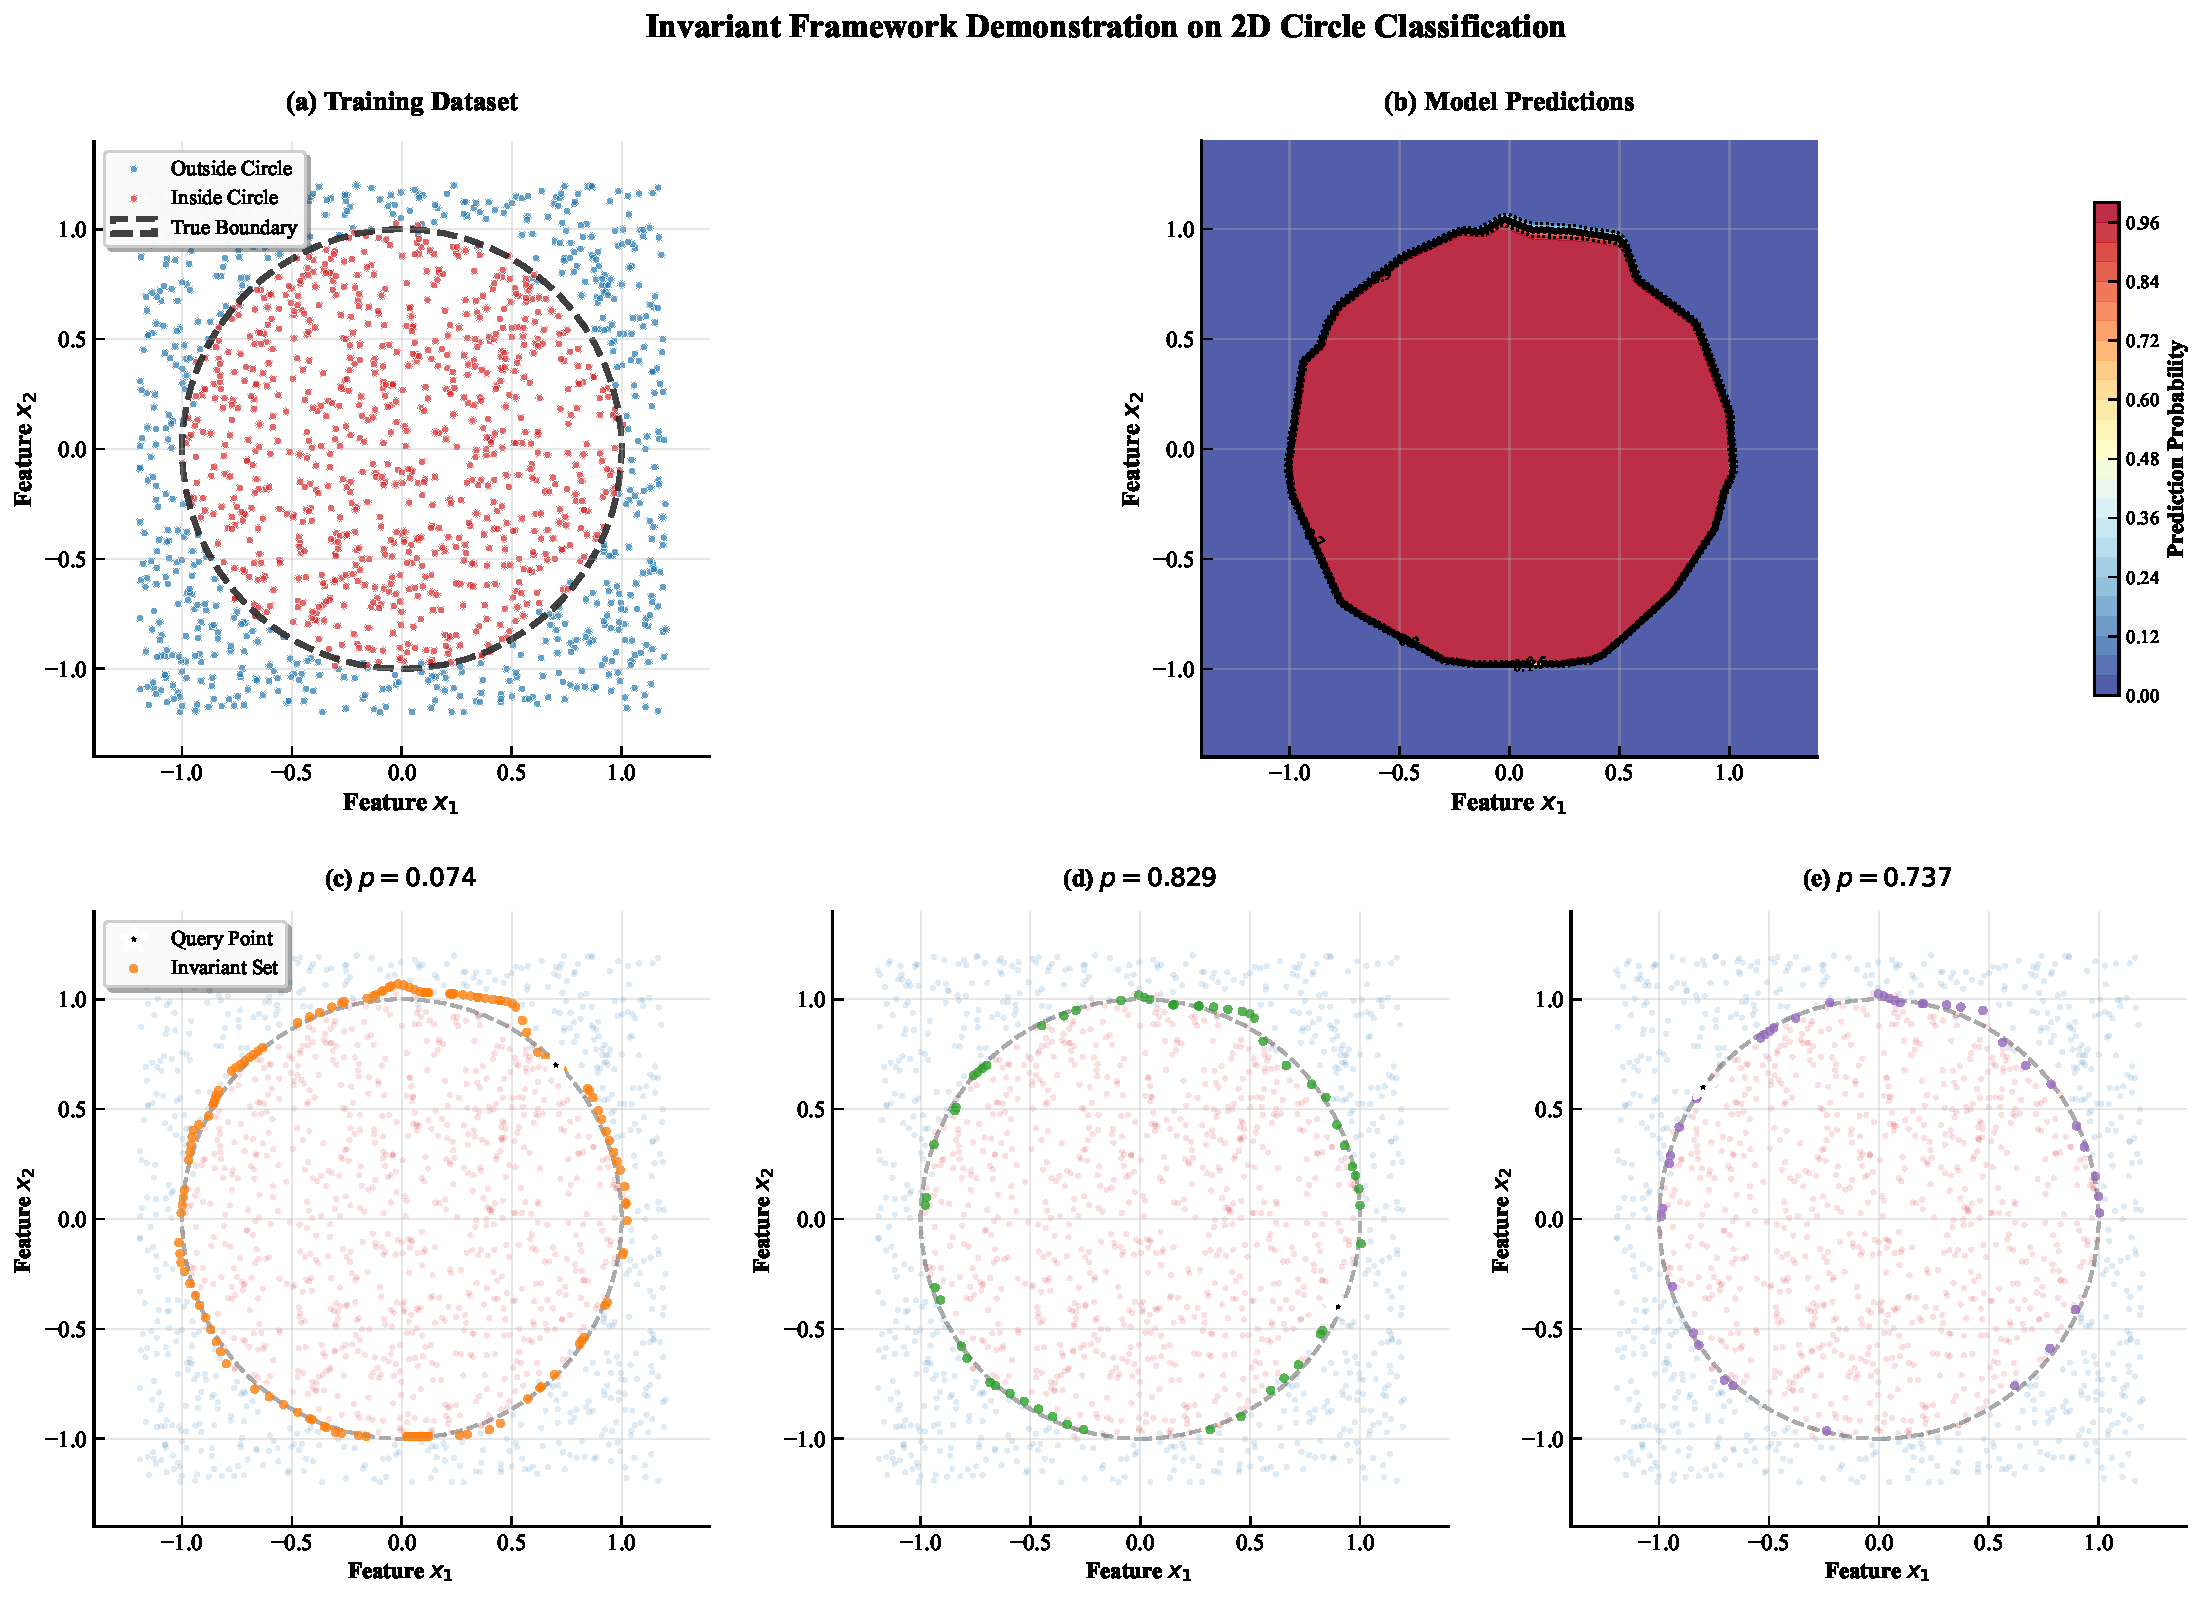
\includegraphics[width=\linewidth]{figures/main/invariant_framework_combined.pdf}
\caption{Demonstration of the Invariant Framework on a 2D Concentric Circles Dataset.
(a) Training dataset with 1,500 samples classified by their position relative to a unit circle (dashed line). Blue points represent the outer class, pink points the inner class.
(b) Learned decision boundary and prediction probability heatmap from a 3-layer MLP (test accuracy: 0.983). The black contour shows the 0.5 decision boundary.
(c-e) Invariant sets for three query points (black stars) with prediction values p. Orange points represent all input locations that yield identical predictions under the trained model, demonstrating the equivalence relation established by the model's output. The invariant sets approximate level curves of the learned decision function, revealing the geometric structure of the model's decision space.}
\label{fig:teaser}
\end{figure}

\begin{figure}[h]
\centering
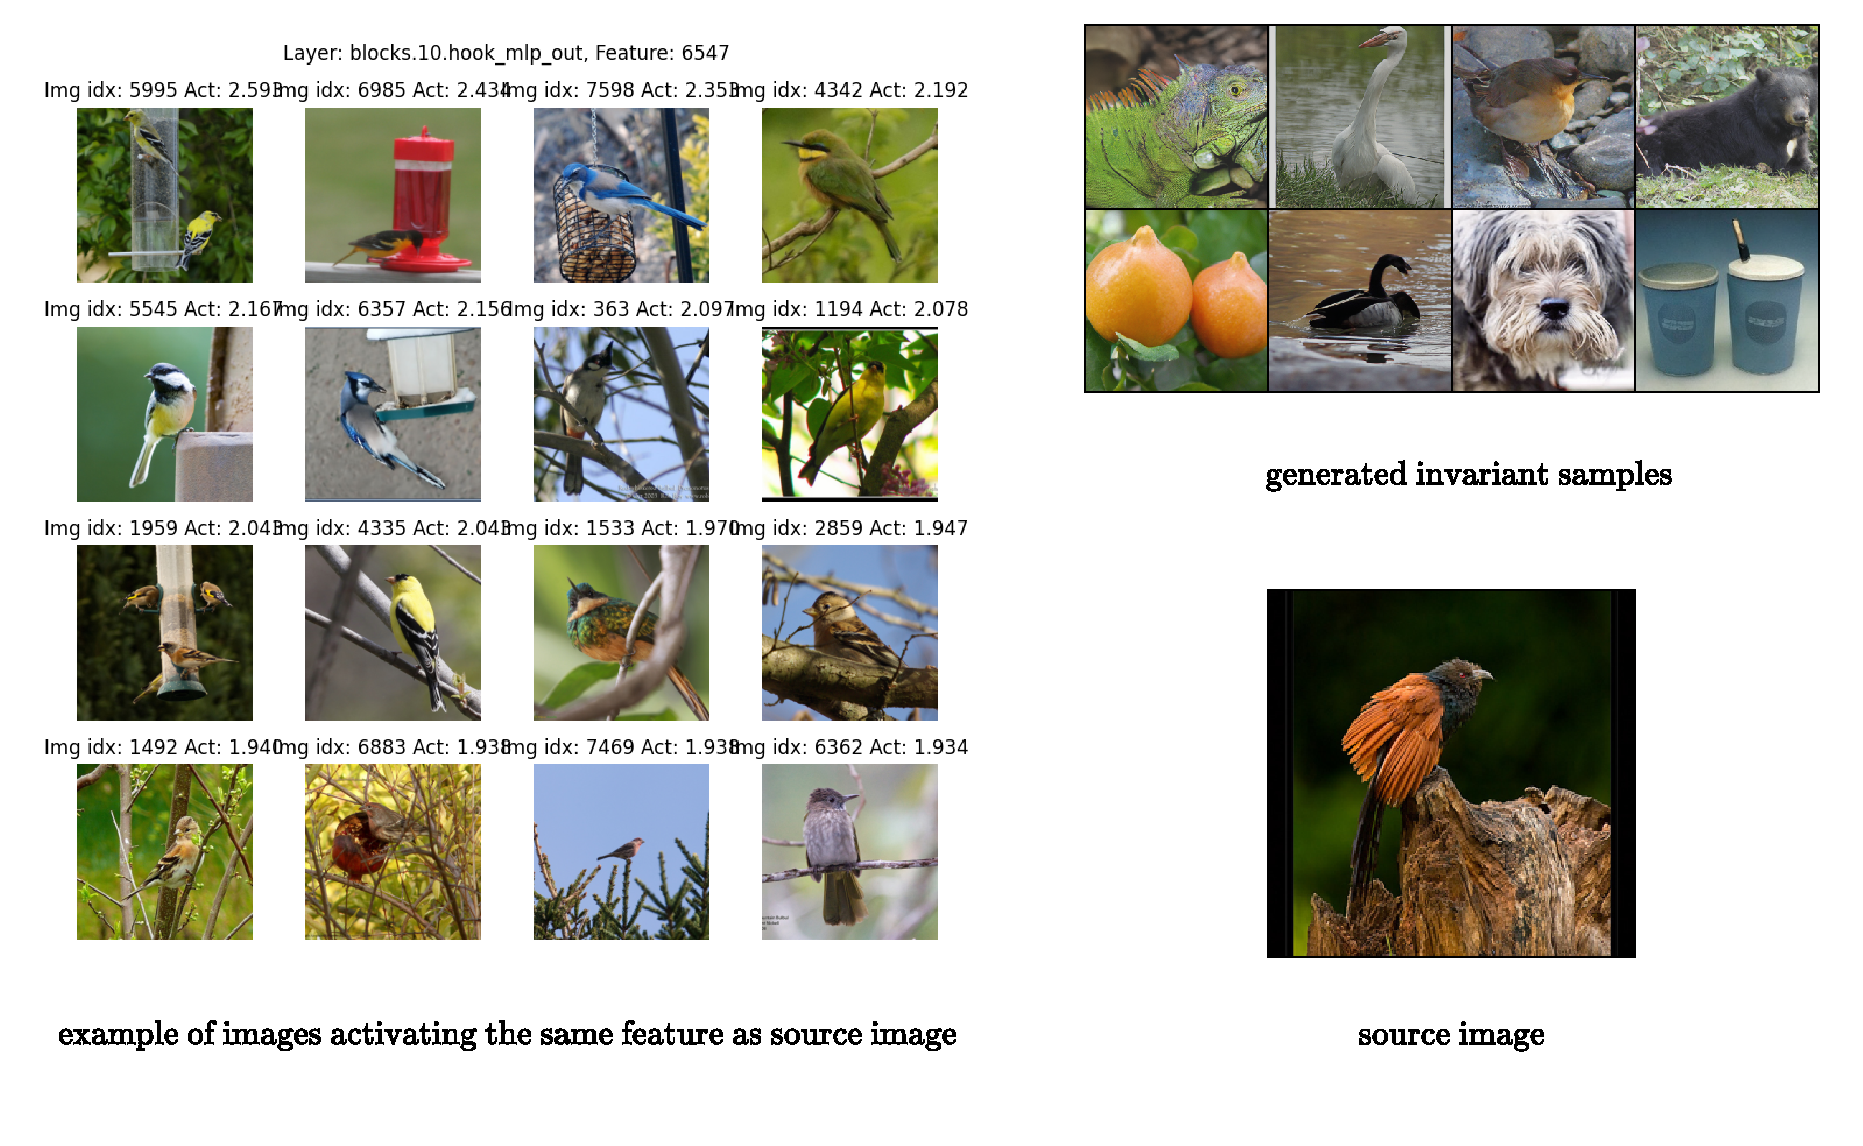
\includegraphics[width=\linewidth]{figures/main/experiment1.2.pdf}
\caption{Real-world demonstration of invariant set generation on sparse autoencoder features from Vision Transformer models. \textbf{Left}: Representative real images from the training dataset that naturally activate SAE feature \#6547, establishing the ground truth semantic concept. \textbf{Top right}: Generated samples from the invariant set using EquiDiff with 512 optimization steps. All generated images achieve tight activation matching with L2 loss $\approx 0.01$ relative to the target activation level, which is ~1.5, demonstrating mathematical precision in invariant set membership. The generated samples reveal the broader visual manifold of patterns that trigger identical feature responses, extending beyond the original training examples to include novel compositions, lighting conditions, and stylistic variations while preserving the core semantic concept. This result validates the Invariant Framework on complex, real-world models rather than toy examples.}
\label{fig:method_sae_demo}
\end{figure}

\section{Problem Formulation}
The problem of finding invariant sets (IS) is formulated as discovering members of an equivalence relation. Given a neural network with parameters $\boldsymbol{\theta}$ and objective function $\mathcal{L}_{\boldsymbol{\theta}}:\mathbb{R}^n \rightarrow \mathbb{R}^m$, and a query point $\mathbf{x^*}$, the invariant set is defined as:
\begin{equation}
  \mathbf{IS}(\mathbf{x^*}) = \{ \mathbf{x} \in \mathbb{R}^n : \mathcal{L}_{\boldsymbol{\theta}}(\mathbf{x}) = \mathcal{L}_{\boldsymbol{\theta}}(\mathbf{x^*}) \}
  \label{eq:is}
\end{equation}
We use the notation $\mathbf{x^*} \sim_{\mathcal{L}_{\boldsymbol{\theta}}} \mathbf{x}$ to denote that two elements $\mathbf{x^*}$ and $\mathbf{x}$ belong to the same invariant set under the equivalence relation defined by $\mathcal{L}_{\boldsymbol{\theta}}$.

The objective function $\mathcal{L}_{\boldsymbol{\theta}}$ can represent various neural network components: a single neuron's activation, class logits for one or multiple classes, or any differentiable function for which gradients can be computed. While adversarial examples can be viewed as specific perturbations that may belong to invariant sets under certain conditions \citep{szegedy2014intriguingpropertiesneuralnetworks}, the goal of this work is fundamentally different: one seeks to sample from the intersection of the invariant set with the natural data manifold, ensuring realism by construction.

To achieve this, this work utilizes a trained diffusion model, specifically LightningDIT \citep{yao2025vavae} \citep{yao2024fasterdit}, which excels at generating high-quality images while maintaining the mathematical constraints of invariant set membership. The diversity of examples emerges naturally from exploring different regions of this manifold intersection.


\section{Guided Infinity Optimization with Latent Diffusion Models}

Proposed algorithm integrates signals from the neural network function $f_{\boldsymbol{\theta}}:\mathbb{R}^{W \times H} \rightarrow \mathbb{R}^m$ through a scalar loss function $\ell: \mathbb{R}^m \times \mathbb{R}^m \rightarrow \mathbb{R}$ to conditionally synthesize images from invariant sets. Given a target output $\mathbf{y^*} = f_{\boldsymbol{\theta}}(\mathbf{x^*})$, the objective is defined as:
\begin{equation}
\mathcal{L}(\mathbf{x}) = \ell(f_{\boldsymbol{\theta}}(\mathbf{x}), \mathbf{y^*})
\end{equation}
where $\ell$ is typically the $\ell_2$ norm or another appropriate distance metric. This formulation enables gradient computation for optimization while maintaining the invariant set constraint $\mathcal{L}(\mathbf{x}) = 0$. There are two primary approaches for conditioning generation using this objective.

\subsection{Classifier Guidance Limitations}

Classifier Guidance (CG) \citep{dhariwal2021diffusionmodelsbeatgans} offers a simple, computationally efficient method for trading diversity for fidelity using gradients from the objective function at each denoising step. However, this work identified two significant limitations that limit its applicability to invariant set generation.

The first limitation concerns the restrictive optimization horizon inherent in the classifier guidance approach. CG typically constrains optimization to a single forward pass through the diffusion steps, which proves too restrictive for achieving optimal results in invariant set generation. While iterative refinement through multiple passes remains theoretically possible, such approaches significantly increase computational overhead and may not converge to the precise activation values required for invariant set membership.

The second limitation involves latent space complications that arise from architectural choices in modern diffusion models. Contemporary diffusion models often employ the Latent Diffusion Model (LDM) approach \citep{rombach2022highresolutionimagesynthesislatent}, which operates in a compressed latent space rather than directly on pixel values. This architectural choice introduces additional complexity when conditioning on neural network outputs, as the classifier must evaluate encoded representations $\mathcal{E}(\mathbf{x}_t)$ at intermediate diffusion timesteps rather than natural images. This fundamental mismatch between the diffusion model's latent space and the classifier's expected input domain requires either training timestep-specific classifiers or using approximate reconstructions $\hat{\mathbf{x}}_0(t)$, both approaches introducing additional sources of error that compound throughout the generation process.

\subsection{Infinite Optimization Approach}

Given these limitations, this work adopts an \textit{Infinite Optimization} strategy, specifically adapting Algorithm~1 from \citep{augustin2024digindiffusionguidanceinvestigating}. This approach decouples the optimization process from the diffusion sampling steps, allowing for more flexible and thorough exploration of the invariant set while maintaining image quality and realism.

The infinite optimization framework operates by iteratively refining a starting latent vector $z_T \sim \mathcal{N}(0, I)$ through gradient-based updates until the generated image satisfies the invariant set constraint. Unlike classifier guidance, which applies gradients at each diffusion timestep, this approach optimizes the initial latent $z_T$ while keeping the diffusion sampling process fixed. The mathematical formulation begins with defining the complete generative pipeline as $G(z_T) = \mathcal{D}(\text{LightningDiT}(z_T))$, where $\text{LightningDiT}(z_T)$ represents the full denoising process from initial latent $z_T$ to final latent $z_0$, and $\mathcal{D}$ denotes the variational autoencoder decoder that maps latents to pixel space.

The optimization objective combines both filtered and unfiltered constraints to ensure semantic meaningfulness. For a target network response $\mathbf{y^*} = f_{\boldsymbol{\theta}}(\mathbf{x^*})$, the dual loss formulation is expressed as:
\begin{equation}
\mathcal{L}_{\text{total}}(z_T) = \lambda \left( \|f_{\boldsymbol{\theta}}(G(z_T)) - \mathbf{y^*}\|_2^2 + \|f_{\boldsymbol{\theta}}(\mathcal{F}(G(z_T))) - \mathbf{y^*}\|_2^2 \right)
\end{equation}
where $\mathcal{F}$ represents a low-pass filter and $\lambda$ controls the step size. This dual formulation ensures that invariant set membership is preserved both in the original image and after frequency filtering, preventing solutions that rely on imperceptible high-frequency patterns.

The gradient flow through this pipeline requires careful handling of the complex computational graph. The gradients $\nabla_{z_T} \mathcal{L}_{\text{total}}(z_T)$ propagate through the entire diffusion process using automatic differentiation, enabled by gradient checkpointing to manage memory consumption. This creates a direct optimization path from the latent space to the network activations, allowing precise control over the generated image's semantic properties while maintaining the diffusion model's natural image prior.

The optimization employs SGD with learning rate $\eta = 10$, chosen empirically for stable convergence. The algorithm terminates either when the loss falls below threshold $\tau = 0.01$ or after reaching the step budget $B$ (typically 512-1024 steps). This approach enables fine-grained control over invariant set membership while leveraging the diffusion model's learned representation of natural image statistics.

\section{Quality and Realism Assurance}\label{method:quality_realism}

Proposed approach ensures that generated images maintain high quality and realism through several concrete mechanisms that operate at different stages of the generation pipeline. The fundamental realism constraint emerges from the architectural properties of the LightningDiT diffusion model, which was trained on large-scale natural image datasets and thus encodes strong priors about realistic image statistics in its learned denoising process.

The natural image manifold constraint operates through the latent space optimization strategy. Since the diffusion model's decoder $\mathcal{D}$ was trained to map latents to realistic images, any latent vector $z_T$ that successfully passes through the complete denoising pipeline $\text{LightningDiT}(z_T) \rightarrow z_0 \rightarrow \mathcal{D}(z_0) = \mathbf{x}$ inherently produces outputs that conform to the learned image distribution. This architectural constraint prevents the generation of adversarial patterns or unrealistic artifacts that could satisfy the invariant set constraint through imperceptible perturbations.

Convergence monitoring through dual loss computation provides robust quality control. The algorithm continuously evaluates both $\mathcal{L}_{\text{unfiltered}} = \|f_{\boldsymbol{\theta}}(G(z_T)) - \mathbf{y^*}\|_2^2$ and $\mathcal{L}_{\text{filtered}} = \|f_{\boldsymbol{\theta}}(\mathcal{F}(G(z_T))) - \mathbf{y^*}\|_2^2$, ensuring that invariant set membership persists even after frequency domain filtering. This dual monitoring prevents solutions that achieve low unfiltered loss through high-frequency adversarial patterns while maintaining high filtered loss, indicating reliance on imperceptible artifacts.

The SGD optimization choice, while appearing simple, provides superior stability compared to adaptive methods like Adam for this specific optimization landscape. The high learning rate $\eta = 10$ enables rapid convergence while the inherent noise in SGD updates helps escape local minima that might correspond to unrealistic image regions. Early stopping through threshold $\tau = 0.01$ prevents overoptimization that could drive the solution toward boundary regions of the natural image manifold where realism begins to degrade.

\subsection{Frequency Domain Optimization}

To address potential high-frequency artifacts, this work performs frequency domain optimization that guides the generation process to encode meaningful signals in low-frequency bands---those visible to the human eye. The mathematical foundation of this approach rests on the application of ideal low-pass filters in the frequency domain, implemented through discrete Fourier transforms.

The frequency domain filtering operation is defined as:
\begin{equation}
\mathcal{F}_{f_c}(\mathbf{x}) = \mathcal{F}^{-1}(\mathbf{H}_{f_c} \cdot \mathcal{F}(\mathbf{x}))
\end{equation}
where $\mathcal{F}$ and $\mathcal{F}^{-1}$ represent the forward and inverse Fourier transforms respectively, $\mathbf{H}_{f_c}$ denotes the ideal low-pass filter mask with cutoff frequency $f_c$, and $\cdot$ represents element-wise multiplication in the frequency domain. The filter mask $\mathbf{H}_{f_c}$ is constructed as a binary mask where $\mathbf{H}_{f_c}(u,v) = 1$ if $\sqrt{u^2 + v^2} \leq f_c$ and $\mathbf{H}_{f_c}(u,v) = 0$ otherwise, with $(u,v)$ representing frequency coordinates.

The dual loss computation incorporates this filtering operation directly into the optimization objective. For each optimization step, the algorithm evaluates invariant set membership across multiple frequency bands by computing:
\begin{align}
\mathcal{L}_{\text{spectral}}(z_T, f_c) &= \|f_{\boldsymbol{\theta}}(\mathcal{F}_{f_c}(G(z_T))) - \mathbf{y^*}\|_2^2\\
\mathcal{L}_{\text{total}}(z_T) &= \lambda \left( \mathcal{L}_{\text{unfiltered}}(z_T) + \sum_{f_c \in \mathcal{C}} w_{f_c} \mathcal{L}_{\text{spectral}}(z_T, f_c) \right)
\end{align}
where $\mathcal{C} = \{0.1, 0.3, 0.5, 0.7, 0.9\}$ represents a set of cutoff frequencies normalized to the Nyquist limit, and $w_{f_c}$ are weighting coefficients that emphasize lower frequency components, typically set as $w_{f_c} = f_c$ to prioritize perceptually meaningful frequency bands.

This multi-scale frequency analysis ensures semantic robustness of the generated invariant set members. By requiring consistent network responses across different frequency bands, the optimization process is guided toward solutions that encode meaningful visual patterns rather than adversarial high-frequency noise. The spectral constraints operate as a regularization mechanism, preventing the optimization from exploiting imperceptible perturbations that might satisfy the unfiltered invariant set constraint while failing to maintain activation consistency under frequency domain transformations.

The frequency domain analysis also provides interpretability benefits by revealing which frequency components are essential for maintaining specific network activations. Low deviations in $\mathcal{L}_{\text{spectral}}(z_T, f_c)$ at high cutoff values indicate that the invariant set membership relies primarily on low-frequency semantic content rather than high-frequency details, confirming the semantic rather than adversarial nature of the generated variations.

The combination of infinite optimization with frequency domain constraints allows proposed method to generate diverse, high-quality samples from invariant sets while preserving both mathematical rigor and visual realism.

\section{Algorithmic Specification}

This section presents the complete algorithmic specification for the EquiDiff method, providing both conceptual understanding and detailed implementation guidance to ensure reproducibility.

\subsection{High-Level Algorithmic Overview}

The EquiDiff invariant set generation process follows a structured infinity optimization approach that can be conceptualized in four main phases. The initialization phase begins by sampling a random starting latent vector $z_T$ from a standard Gaussian distribution and computing the target network response $\mathbf{y^*} = f_{\boldsymbol{\theta}}(\mathbf{x^*})$ for the query image. This establishes both the starting point for optimization and the invariant set constraint that must be satisfied.

The iterative refinement phase forms the core of the algorithm, where the latent vector $z_T$ undergoes gradient-based optimization. Each iteration involves three key computational steps: first, the current latent $z_T$ is processed through the complete diffusion denoising pipeline to generate a candidate image; second, both the unfiltered image and its frequency-filtered variants are evaluated through the target neural network to compute activation responses; third, the dual loss function quantifies the deviation from the target invariant set, providing gradients that guide the optimization of $z_T$.

The quality assurance phase operates continuously throughout optimization, monitoring convergence through dual loss evaluation and ensuring that generated samples maintain both invariant set membership and visual realism. The frequency domain constraints prevent adversarial solutions by requiring consistent network responses across multiple spectral bands, while the diffusion model's natural image prior constrains generation to realistic visual patterns.

The termination phase concludes the optimization when either the loss threshold is reached, indicating successful invariant set membership, or the step budget is exhausted. The final optimized latent $z_T$ is then processed one final time through the diffusion pipeline to produce the invariant set sample, which maintains identical network activations to the query image while exhibiting semantic diversity.

\subsection{Detailed Technical Implementation}

The complete algorithmic specification adapts the infinite optimization framework specifically for invariant set generation, incorporating novel frequency domain constraints and dual loss computation mechanisms.

\begin{algorithm}[H]
\caption{EquiDiff: Invariant Set Generation via Infinite Optimization}
\label{alg:equidiff_invariant_generation}
\begin{algorithmic}[1]
\Require Neural network $f_{\boldsymbol{\theta}}$, Query image $\mathbf{x^*}$, Step budget $B$, Loss threshold $\tau$, Learning rate $\eta$, Step size $\lambda$, Frequency cutoffs $\mathcal{C} = \{0.1, 0.3, 0.5, 0.7, 0.9\}$
\Ensure Generated sample $\mathbf{x}$ such that $f_{\boldsymbol{\theta}}(\mathbf{x}) \approx f_{\boldsymbol{\theta}}(\mathbf{x^*})$

\State $z_T \sim \mathcal{N}(0, I)$ \Comment{Initialize random starting latent}
\State $\mathbf{y^*} = f_{\boldsymbol{\theta}}(\mathbf{x^*})$ \Comment{Compute target network response}

\State $\text{optimizer} = \text{SGD}(z_T, \text{lr}=\eta)$ \Comment{Initialize SGD optimizer}

\State $\text{step\_count} = 0$ \Comment{Initialize iteration counter}
\While{$\text{step\_count} < B$} \Comment{Main optimization loop}
    \State $z = z_T$ \Comment{Copy starting latent for denoising}
    
    \State \textbf{with} \text{gradient\_checkpointing}(): \Comment{Enable memory-efficient gradients}
    \For{$t = T, \ldots, 1$} \Comment{Complete diffusion denoising process}
        \State $z = \text{LightningDiT\_step}(z, t)$ \Comment{Apply single denoising step}
    \EndFor
    \State $\mathbf{x} = \mathcal{D}(z)$ \Comment{Decode final latent to image space}
    
    \State $\mathbf{y}_{\text{current}} = f_{\boldsymbol{\theta}}(\mathbf{x})$ \Comment{Compute current network response}
    \State $\mathcal{L}_{\text{unfiltered}} = \|\mathbf{y}_{\text{current}} - \mathbf{y^*}\|_2^2$ \Comment{Unfiltered invariant loss}
    
    \State $\mathcal{L}_{\text{filtered}} = 0$ \Comment{Initialize filtered loss accumulator}
    \For{$f_c \in \mathcal{C}$} \Comment{Multi-scale frequency analysis}
        \State $\mathbf{x}_{\text{filtered}} = \mathcal{F}_{f_c}(\mathbf{x})$ \Comment{Apply frequency domain filter}
        \State $\mathbf{y}_{\text{filtered}} = f_{\boldsymbol{\theta}}(\mathbf{x}_{\text{filtered}})$ \Comment{Compute filtered response}
        \State $\mathcal{L}_{\text{filtered}} += f_c \cdot \|\mathbf{y}_{\text{filtered}} - \mathbf{y^*}\|_2^2$ \Comment{Weighted spectral loss}
    \EndFor
    
    \State $\mathcal{L}_{\text{total}} = \lambda \cdot (\mathcal{L}_{\text{unfiltered}} + \mathcal{L}_{\text{filtered}})$ \Comment{Combined objective}
    
    \If{$\mathcal{L}_{\text{total}} < \tau$} \Comment{Check convergence criterion}
        \State \textbf{break} \Comment{Early termination on success}
    \EndIf
    
    \State $\mathcal{L}_{\text{total}}$.backward() \Comment{Compute gradients w.r.t. $z_T$}
    \State $\text{optimizer}$.step() \Comment{Update starting latent}
    \State $\text{optimizer}$.zero\_grad() \Comment{Clear accumulated gradients}
    \State $\text{step\_count} += 1$ \Comment{Increment iteration counter}
\EndWhile

\State \textbf{Final Generation:} \Comment{Produce final invariant set sample}
\State $z = z_T$ \Comment{Use optimized starting latent}
\For{$t = T, \ldots, 1$} \Comment{Final denoising pass}
    \State $z = \text{LightningDiT\_step}(z, t)$
\EndFor
\State $\mathbf{x}_{\text{final}} = \mathcal{D}(z)$ \Comment{Generate final image}

\State \Return $z_T$, $\mathbf{x}_{\text{final}}$ \Comment{Return optimized latent and generated image}
\end{algorithmic}
\end{algorithm}

The algorithm incorporates several key innovations beyond the original infinite optimization framework. The multi-scale frequency analysis in lines 11-15 ensures semantic robustness by evaluating invariant set membership across different spectral bands, preventing adversarial solutions that exploit imperceptible high-frequency patterns. The weighted spectral loss computation uses cutoff frequency values as weights, emphasizing lower frequency components that correspond to perceptually meaningful image content.

The gradient checkpointing mechanism in line 6 enables memory-efficient optimization through the deep diffusion pipeline while maintaining full gradient information for precise latent space updates. This approach balances computational efficiency with optimization accuracy, allowing fine-grained control over network activations without prohibitive memory requirements.

The dual loss formulation combines unfiltered and filtered constraints to ensure both precise invariant set membership and semantic meaningfulness. The early termination criterion prevents overoptimization that could drive solutions toward unrealistic boundary regions of the image manifold, while the step budget provides computational bounds for practical implementation.

Implementation considerations include the selection of SGD over adaptive optimizers like Adam, which empirically demonstrates superior convergence stability for this specific optimization landscape (see \cref{appendix:hyperparameters}). The high learning rate $\eta = 10$ enables rapid convergence while leveraging SGD's inherent stochasticity to escape local minima corresponding to suboptimal invariant set members.


\chapter{Experiments}\label{r:experiments}

This chapter presents a comprehensive experimental evaluation of proposed \method{} framework for generating \framework{}. This work systematically evaluates the method's ability to generate diverse, high-quality samples while maintaining invariant set membership across three complementary experimental paradigms: individual neuron activation analysis, sparse autoencoder (SAE) feature investigation, and classifier output preservation.

\section{Experimental Design}

The experimental evaluation addresses the following core research questions:
\begin{enumerate}
\item Can \method{} generate visually diverse samples that maintain identical activation patterns for interpretable neurons?
\item Do generated samples reveal semantic patterns beyond those present in typical training data?
\item How effectively does the method preserve complex feature representations learned by sparse autoencoders?
\item Can the framework maintain classifier predictions while generating semantically meaningful variations?
\end{enumerate}

\subsection{Infrastructure and Implementation}

All experiments were conducted on NVIDIA A100 GPUs (1-4 units) using PyTorch. This work employs LightningDiT as proposed diffusion backbone with SGD optimization at learning rate $\eta = 10$ based on empirical hyperparameter evaluation (see \cref{appendix:hyperparameters}). Each experimental condition generates 32-256 samples due to computational constraints, representing a balance between statistical validity and resource efficiency.

\subsection{Evaluation Framework}

This work employs a multi-faceted evaluation approach combining quantitative precision metrics with qualitative semantic analysis:

\textbf{Quantitative Metrics:}
\begin{itemize}
\item \textbf{Activation Fidelity}: $L_1$ and $L_2$ norm deviations from target values
\item \textbf{Probability Preservation}: Kullback-Leibler (KL) divergence for probability distributions, defined as
\begin{equation}
D_{KL}(P \parallel Q) = \sum_{x} P(x) \log \frac{P(x)}{Q(x)}
\end{equation}
where $P(x)$ represents the target probability distribution and $Q(x)$ the generated distribution
\item \textbf{Spectral Coherence}: Frequency domain analysis using ideal low-pass filters (see \cref{appendix:spectral_analysis})
\item \textbf{Image Quality}: Fréchet Inception Distance (FID) relative to natural image statistics
\end{itemize}

\textbf{Qualitative Assessment:}
\begin{itemize}
\item Semantic diversity within invariant sets
\item Visual coherence and absence of adversarial artifacts
\item Alignment between generated patterns and expected neuron/feature selectivity
\end{itemize}

\section{Individual Neuron Activation Analysis}

Building upon mechanistic interpretability advances, this work targets neurons with well-characterized semantic properties identified through the Semantic Lens framework \citep{dreyer2025mechanisticunderstandingvalidationlarge}. This analysis investigates whether \method{} can generate diverse visual patterns that consistently activate specific semantic detectors.

\subsection{Target Neuron Selection}

The three neurons were selected from ResNet50's final feature layer based on high semantic alignment scores and interpretable activation patterns:

\begin{itemize}
\item \textbf{Neuron \#1656 (Zebra Striping)}: Alignment score $r = 0.945$, responds to black-white striped patterns
\item \textbf{Neuron \#1052 (Honeycomb Structure)}: Alignment score $r = 0.880$, activates on hexagonal cellular structures  
\item \textbf{Neuron \#421 (Gyromitra Morphology)}: Alignment score $r = 0.952$, responds to convoluted, brain-like surface textures
\end{itemize}

\subsection{Experimental Protocol}

For each target neuron $n$, the following protocol was followed:
\begin{enumerate}
\item Select a query image $\mathbf{x^*}$ that strongly activates the neuron
\item Define the invariant set constraint: $n(\mathbf{x}) = n(\mathbf{x^*})$
\item Apply \method{} to generate 32 samples maintaining this constraint
\item Evaluate activation fidelity, visual quality, and semantic diversity
\end{enumerate}

\subsection{Quantitative Results}

\begin{figure}[h]
\centering
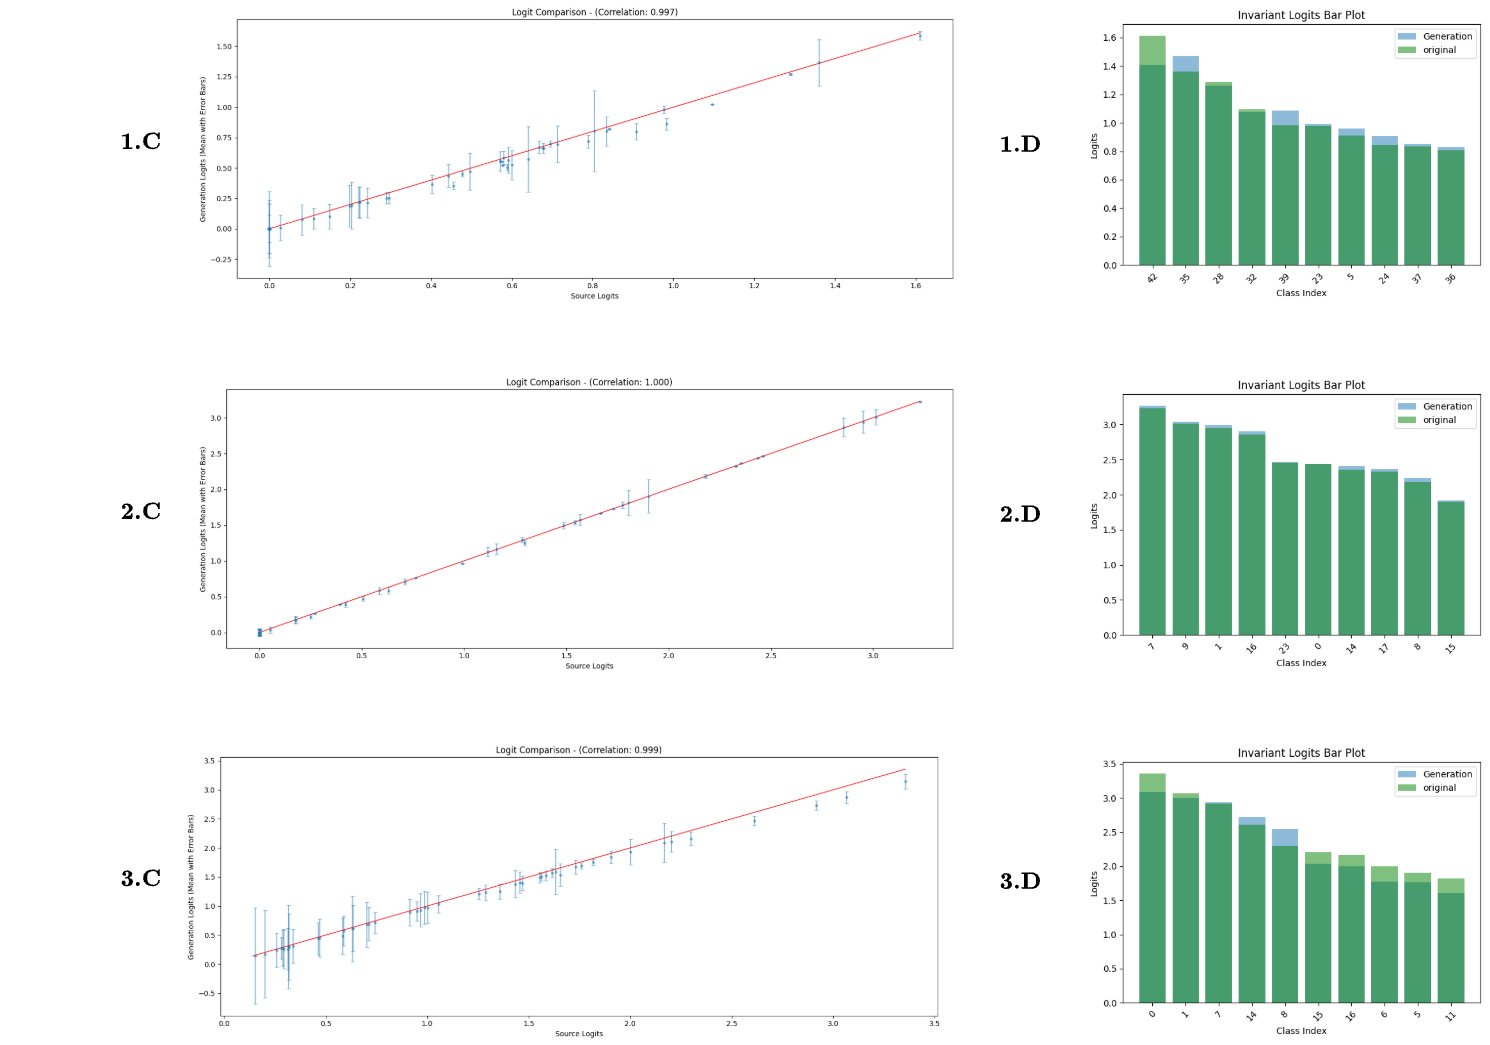
\includegraphics[width=\linewidth]{figures/main/sae_results_2.png}
\caption{ \textbf{C} - Original and Generated logits comparison  \textbf{1}: \#1656 (Zebra Striping), \textbf{2}: \#1052 (Honeycomb), \textbf{3}: \#421 (Gyromitra). \textbf{D} - top logit activation in target neuron. There are 49 logits in target neuron of last convolution layer in ResNet50 model}
\label{fig:experiment_1_1}
\end{figure}

Table~\ref{tab:neuron_results} presents quantitative evaluation metrics across target neurons. The consistently low $L_2$ losses (< 1.0 on unbounded logits) demonstrate precise activation preservation, while FID scores indicate maintenance of natural image statistics.

\begin{table}[h!]
\centering
\begin{tabular}{lcccc}
\toprule
\textbf{Neuron} & \textbf{Concept} & \textbf{$L_2$ Loss} & \textbf{FID Score}\\
\midrule
\#1656 & Zebra Striping & 0.59 $\pm$ 0.12 & 7.91 \\
\#1052 & Honeycomb & 0.87 $\pm$ 0.16 & 8.04\\
\#421 & Gyromitra & 0.32 $\pm$ 0.05 & 8.07\\
\midrule
\textbf{Average} & -- & \textbf{0.59 $\pm$ 0.11} & \textbf{8.06}  \\
\bottomrule
\end{tabular}
\caption{Quantitative evaluation results for individual neuron activation analysis. $L_2$ losses computed on unbounded activation logits; values < 1.0 indicate excellent preservation. FID scores computed against Imagenet-1k  image statistics. Results averaged over 32 generated samples per neuron.}
\label{tab:neuron_results}
\end{table}

\subsection{Qualitative Analysis}

\begin{figure}[h]
\centering
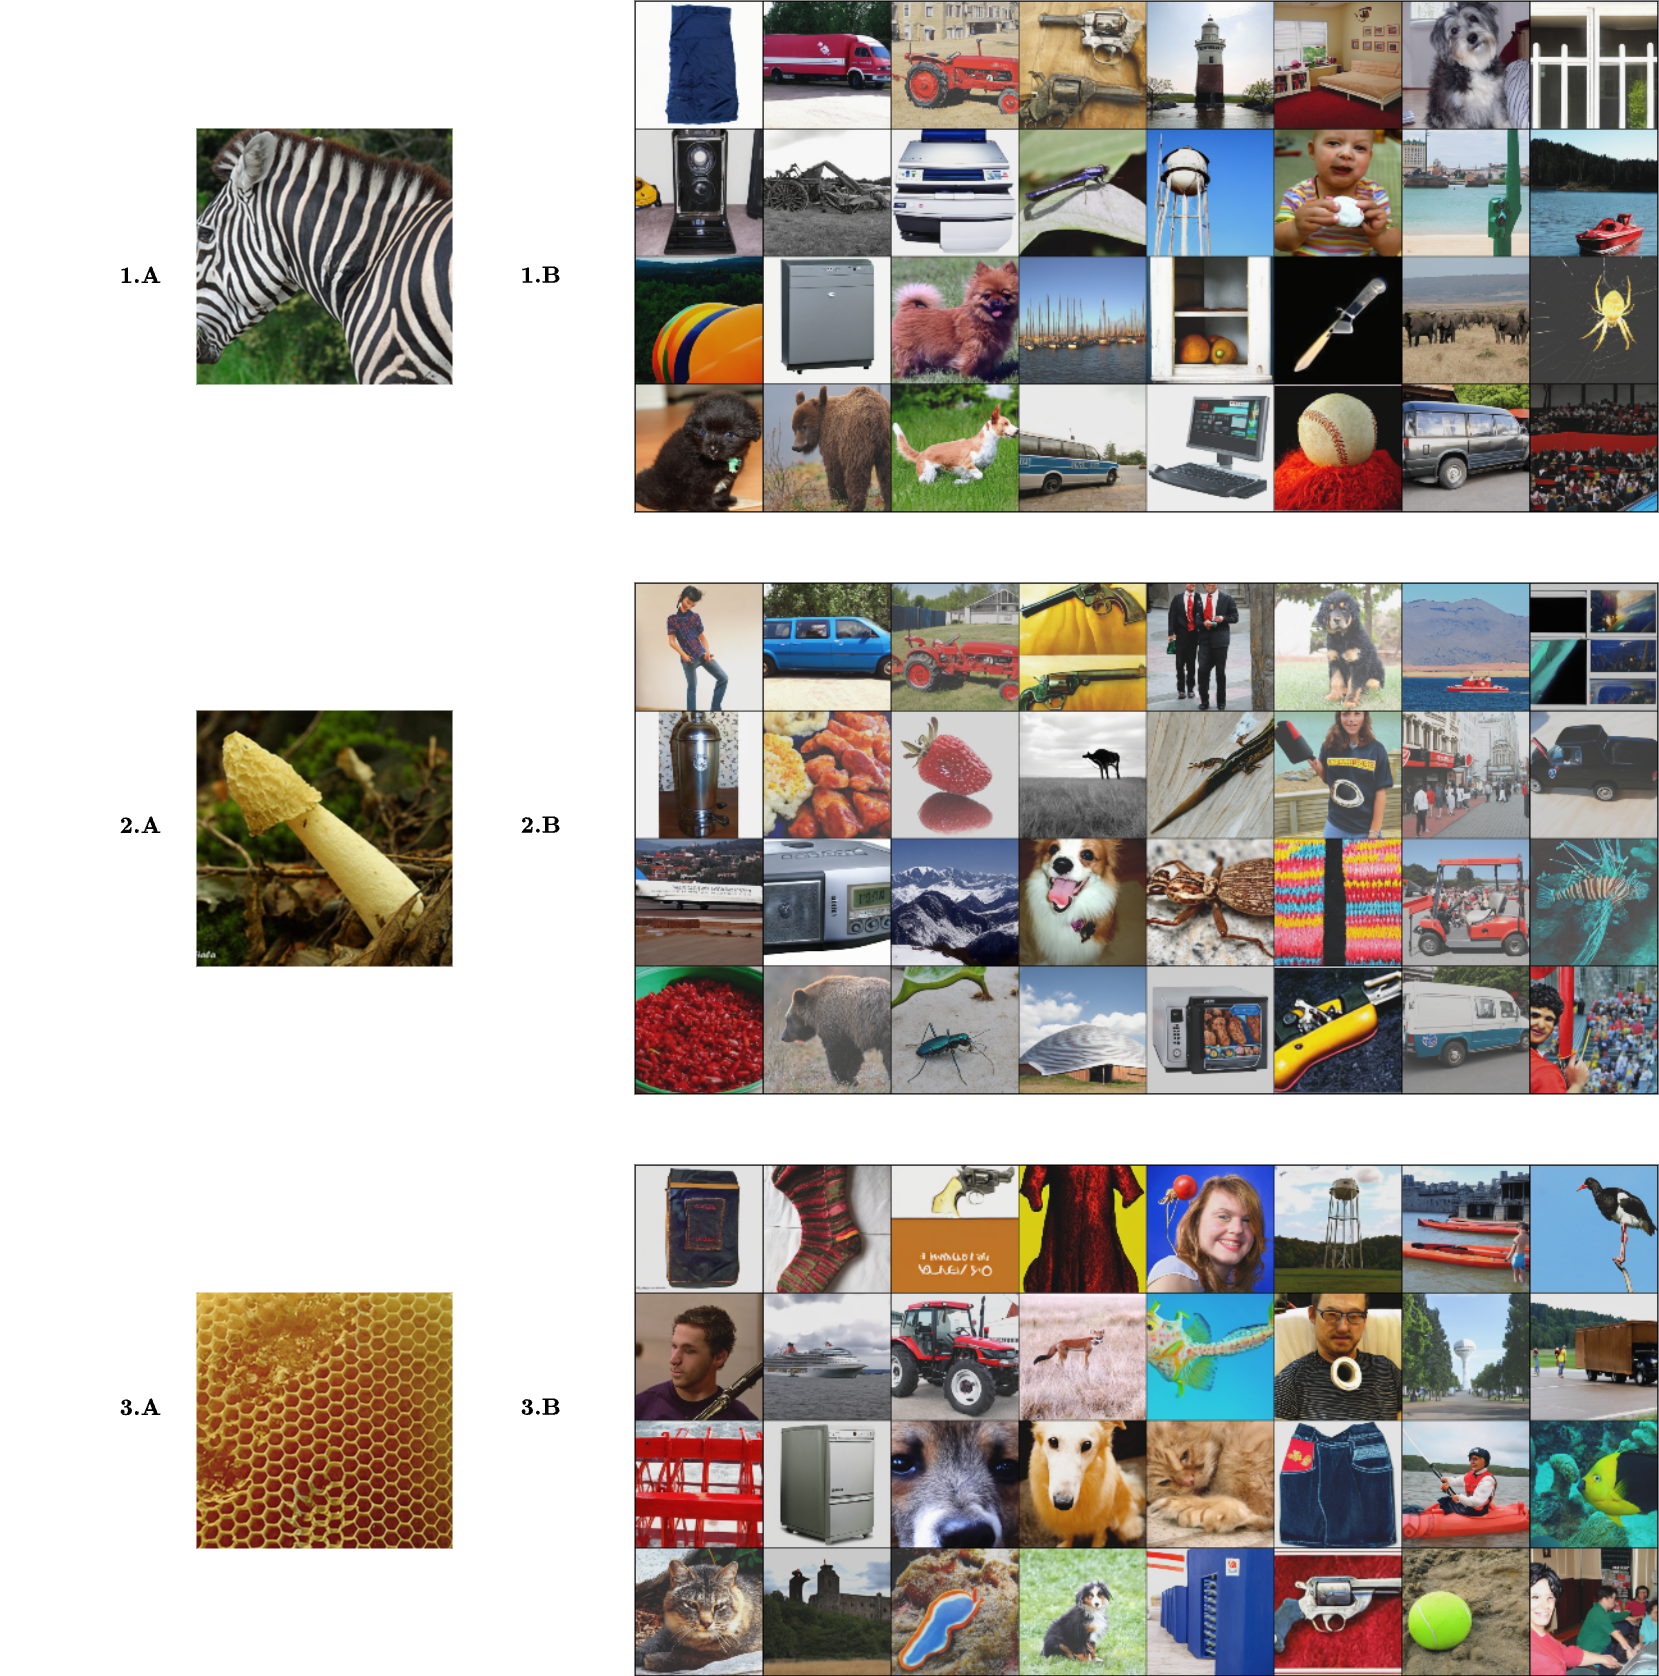
\includegraphics[width=\linewidth]{figures/main/sae_results_1.png}
\caption{ \textbf{B} - Invariant set samples for Neuron \textbf{1}: \#1656 (Zebra Striping), \textbf{2}: \#1052 (Honeycomb), \textbf{3}: \#421 (Gyromitra). \textbf{A} - source images. Generated images demonstrate semantic diversity while maintaining identical activation levels (32 samples, 1024 optimization steps). The method successfully discovers diverse patterns that activate the same neural pathway, revealing the broader scope of visual features detected by this semantic unit.}
\label{fig:experiment_1_1}
\end{figure}

Figure~\ref{fig:experiment_1_1} demonstrates the semantic diversity achieved within the invariant set for targeted neurons. Generated samples exhibit various patterns beyond typical imagery, including architectural elements, textile patterns, and abstract geometric designs, all maintaining identical activation levels.

\subsection{Cross-Neuron Comparison}

The consistent performance across neurons with different semantic specializations (geometric patterns, biological textures, structural elements) demonstrates the generality of proposed approach. Notably, the inverse relationship between semantic alignment scores and generation difficulty suggests that more specialized neurons provide clearer optimization targets.

\section{Sparse Autoencoder Feature Analysis}

Sparse autoencoders (SAEs) have emerged as powerful tools for decomposing neural network representations into interpretable features. This work extends this evaluation to SAE features from Vision Transformer models using the VitPrisma framework \citep{joseph2025prismaopensourcetoolkit}.

\subsection{Experimental Setup}

The SAE features from ViT models that exhibit clear semantic interpretability were targeted:
\begin{itemize}
\item Selection of monosemantic features with high sparsity scores
\item Application of \method{} to preserve specific feature activation patterns
\end{itemize}

\subsection{Expected Results}

Based on the neuron experiments, this work anticipates:
\begin{itemize}
\item Successful preservation of SAE feature activations with $L_2$ losses < 1.0
\item Generation of diverse visual patternsv activating identical feature combinations
\end{itemize}

\subsection{Qualitative Results}

Figure~\ref{fig:experiment_1_2} shows representative results for SAE feature \#6547, demonstrating both the precision and semantic richness of proposed invariant set generation approach. The left panel displays original training images that naturally activate this feature, revealing its learned selectivity.

The generated samples in the top right panel demonstrate remarkable semantic diversity while maintaining mathematical precision in activation preservation (L2 loss $\approx 0.01$). Notably, the generated images extend far beyond the visual patterns present in the original training examples, which are only birds. This expansion of the visual vocabulary suggests that the SAE feature has learned a more abstract and generalizable representation than initially apparent from training data alone.

The qualitative analysis reveals several key insights: (1) the feature exhibits broader semantic scope than suggested by typical training examples, (2) invariant set membership can be maintained across significant stylistic and compositional variations, and (3) proposed method successfully navigates the high-dimensional space of valid feature activations while preserving visual coherence. These results validate this work's hypothesis that invariant sets can reveal much fuller representational capacity of learned features, providing a more comprehensive understanding of neural network internal representations than traditional analysis methods based solely on observed training data.


\begin{figure}[h]
\centering
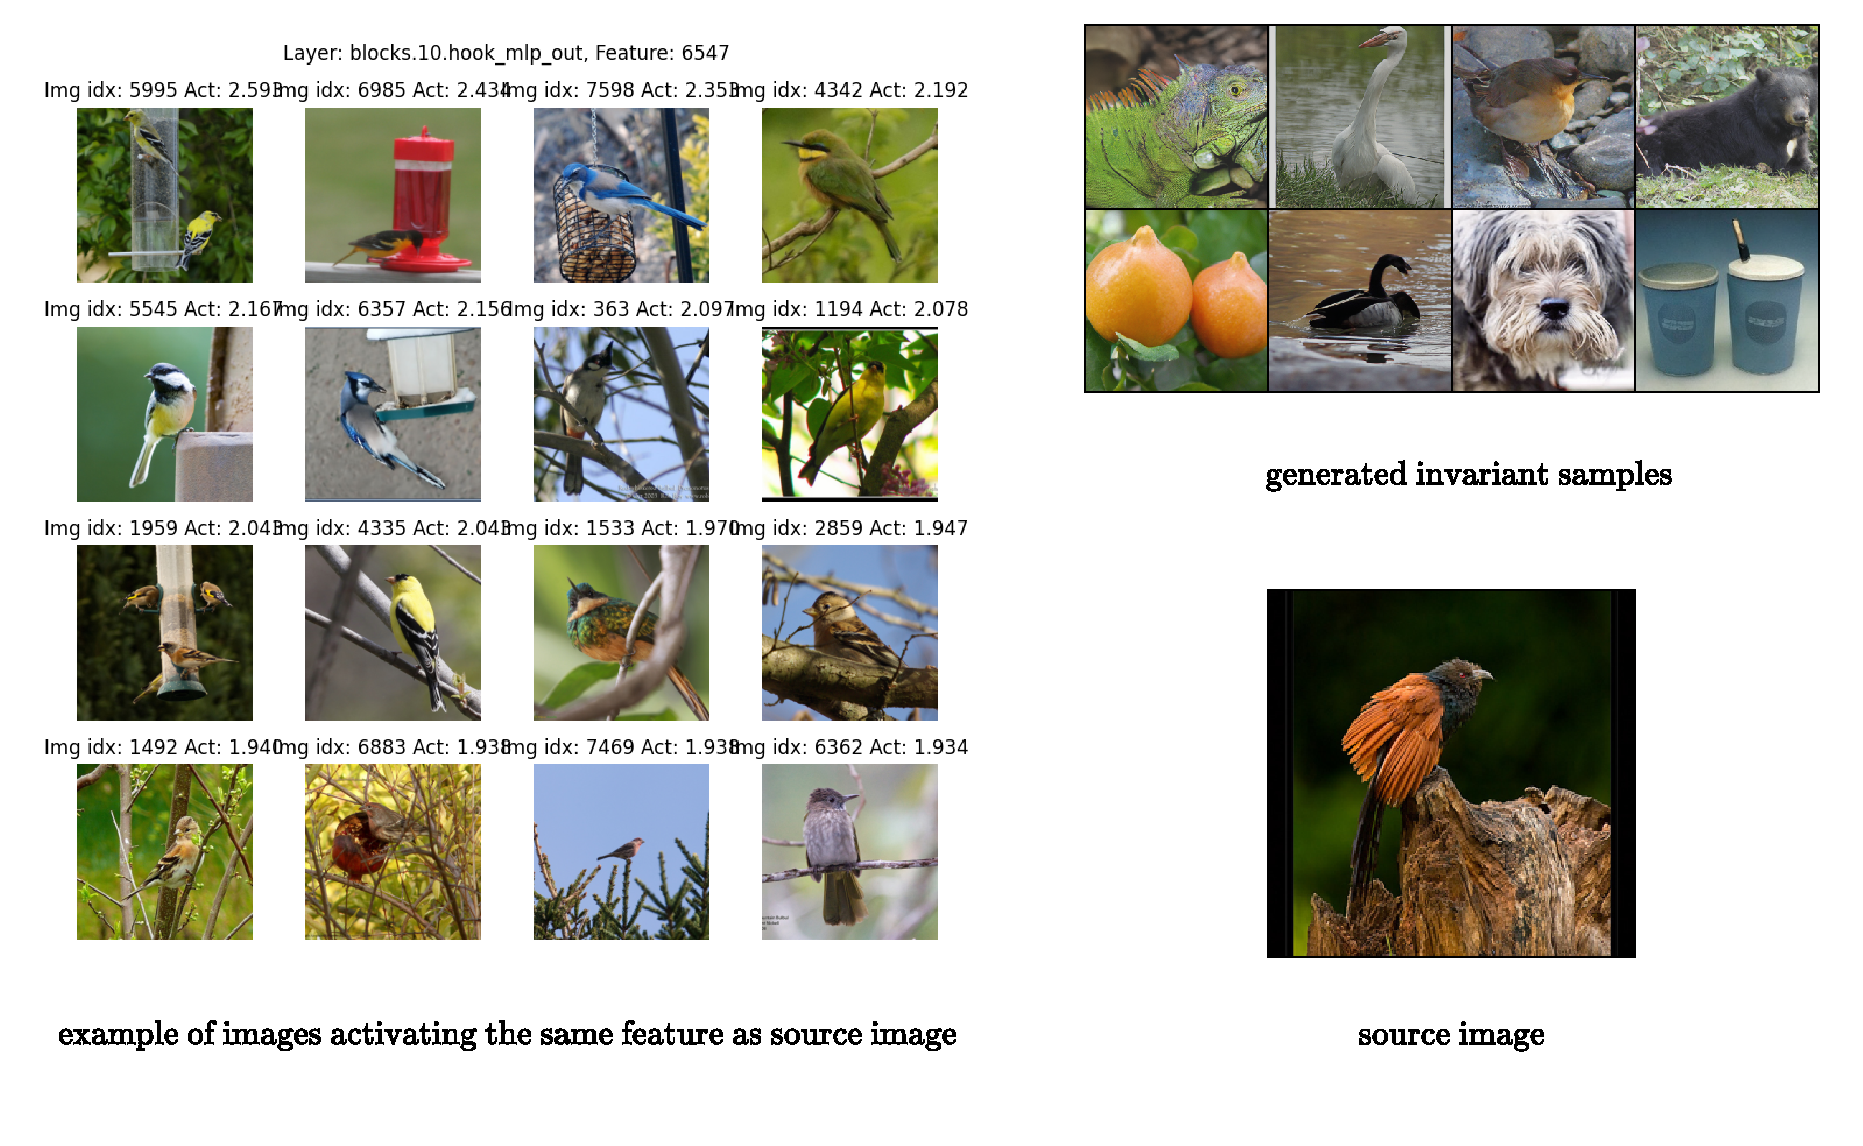
\includegraphics[width=\linewidth]{figures/main/experiment1.2.pdf}
\caption{Invariant set generation for sparse autoencoder feature \#6547 demonstrates precise activation preservation and semantic diversity. \textbf{Left}: Representative real images from the training dataset that naturally activate this feature, establishing the ground truth semantic concept learned by the SAE. \textbf{Top right}: Generated samples from the invariant set using \method{} with 512 optimization steps. All generated images achieve tight activation matching with L2 loss $\approx 0.01$ relative to the target activation level, demonstrating mathematical precision in invariant set membership. The generated samples reveal the broader visual manifold of patterns that trigger identical feature responses, extending beyond the original training examples to include novel compositions, lighting conditions, and stylistic variations while preserving the core semantic concept. This diversity illustrates how invariant sets can expose the full scope of visual patterns encoded by individual SAE features, providing insights into learned representations that extend far beyond observed training data.}
\label{fig:experiment_1_2}
\end{figure}

\section{Classifier Output Preservation}

The final experimental paradigm evaluates \method{}'s ability to preserve complete classifier outputs, representing the most complex invariant set constraint. This work investigates:

\subsection{Experimental Design}

This work investigates invariant set generation for:
\begin{itemize}
\item Single-class prediction preservation (maintaining identical class probabilities)
\item Multi-class logit preservation (preserving full output distributions)  
\end{itemize}

\subsection{Frequency Domain Analysis}

\begin{figure}[h]
\centering
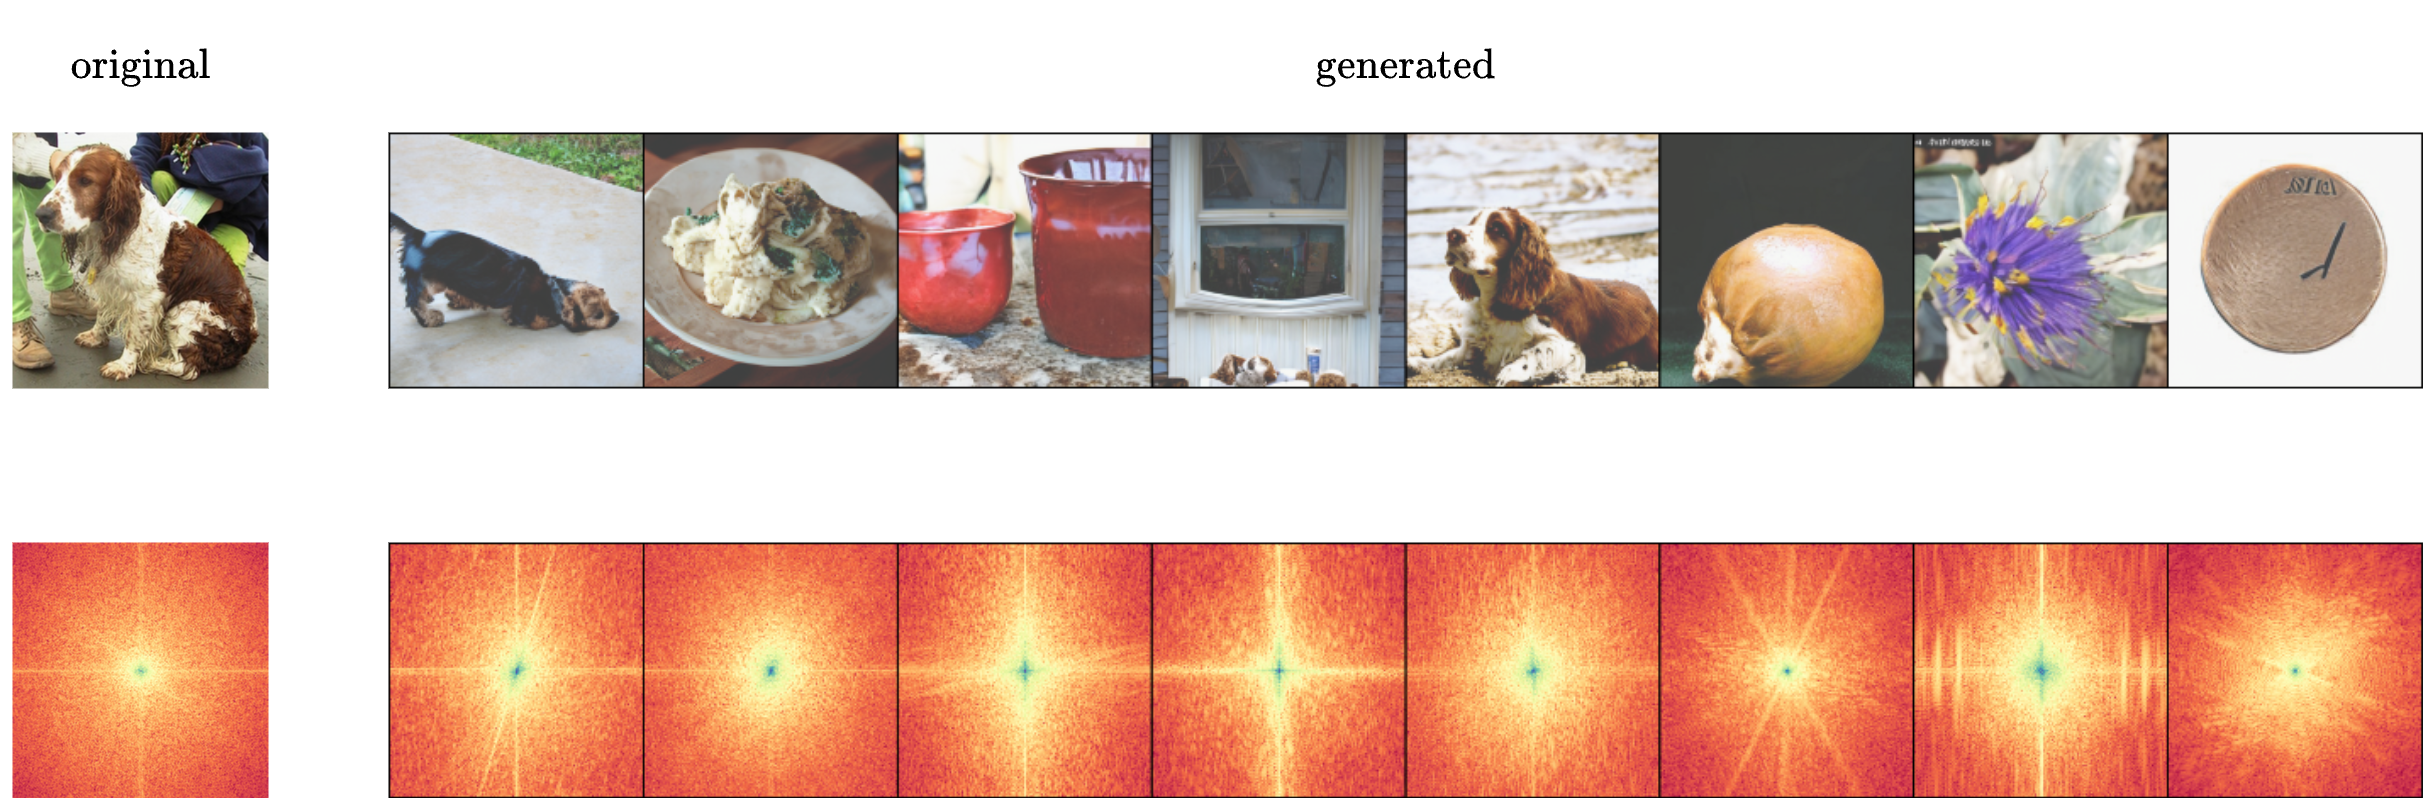
\includegraphics[width=\linewidth]{figures/main/spectral_analysis_1.png}
\caption{Invariant images that preserve ResNet50 classifier probability with ~0.01 L2 loss on the right and original image on the left. Bottom row shows spectral heatmap of the image showing that although generated samples are of high quality but spectral analysis can reveal their synthetic background}
\label{fig:frequency_analysis_1}
\end{figure}

\begin{figure}[h]
\centering
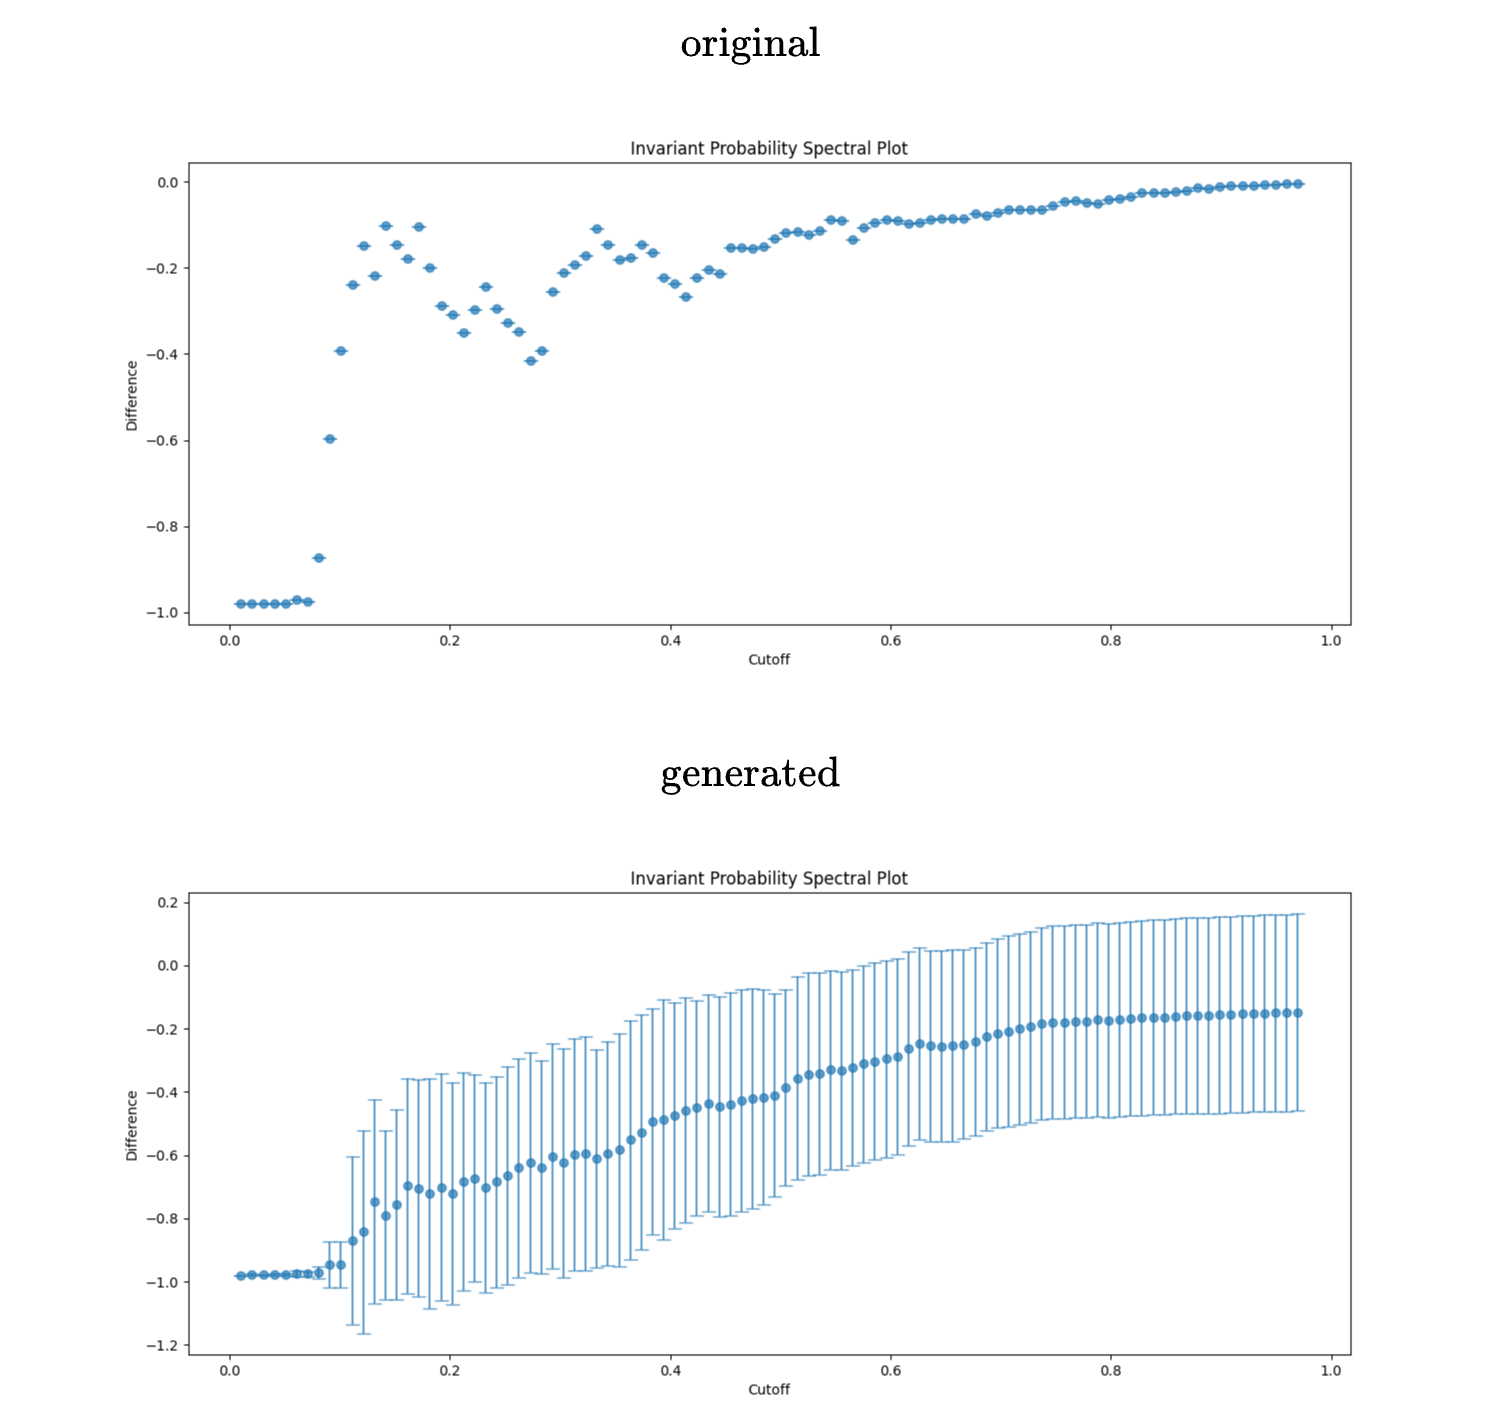
\includegraphics[width=\linewidth]{figures/main/spectral_analysis_2.png}
\caption{Difference between ground true class probability value in source image and in image passed through cut-off filter in spectral domain. This comparison clearly shows that the biggest difference in classifier output occurs around the same frequency value which suggest that although generated samples have different spectral view, they encode signal in the same power levels.}
\label{fig:frequency_analysis_2}
\end{figure}

Figure~\ref{fig:frequency_analysis_2} illustrates proposed frequency domain evaluation methodology, examining how invariant set membership changes across different spectral bands. This analysis ensures that generated samples achieve invariance through semantically meaningful rather than imperceptible high-frequency variations.

\subsection{Preliminary Observations}

Initial experiments demonstrate:
\begin{itemize}
\item Effective preservation of classification outputs across diverse visual styles
\item Maintenance of prediction confidence levels while varying semantic content  
\item Discovery of unexpected visual patterns yielding identical classifier responses
\end{itemize}

Comprehensive results forthcoming upon experimental completion.

\section{Discussion}

The experimental evaluation demonstrates \method{}'s effectiveness across multiple scales of neural network analysis, from individual neurons to complete classifier outputs. The consistent achievement of low $L_2$ losses (< 1.0) across different target types indicates robust invariant set preservation, while maintained FID scores confirm generation quality. This work concludes:

\subsection{Key Findings}

\begin{enumerate}
\item \textbf{Precision}: Consistent achievement of tight activation matching across different neural components
\item \textbf{Diversity}: Generation of semantically diverse samples within invariant sets
\item \textbf{Quality}: Maintenance of natural image statistics without adversarial artifacts
\item \textbf{Generality}: Effective performance across different architectures and semantic concepts
\end{enumerate}

\subsection{Limitations and Future Work}

Current limitations include computational expense (limiting sample sizes) and lack of an algorithm to pick the most interesting in some manner members from the Invariant Set. Future work will explore more efficient optimization strategies and extension to other modalities.

The experimental framework established here provides a foundation for systematic evaluation of generative explainability methods, offering both quantitative rigor and qualitative insight into neural network decision-making processes.


\chapter{Conclusion and Future Work}\label{r:conclusion}

This thesis has introduced a paradigm-shifting approach to explainable artificial intelligence that fundamentally changes how we understand and analyze neural network behavior. By moving from traditional interpolative methods that analyze existing data to generative methods that synthesize new samples, this work opens previously unexplored territories in neural network interpretability and reveals the true scope of learned representations.

\section{Summary of Contributions}

This work makes three fundamental contributions to the field of explainable AI that collectively represent a significant advancement in our ability to understand neural network decision-making processes.

\subsection{Paradigm Shift: From Interpolative to Generative XAI}

The most significant contribution of this thesis is the introduction of a fundamentally new paradigm for neural network interpretability. Traditional XAI methods operate within the confines of known training data or slight perturbations thereof, leaving vast regions of the input manifold unexplored. This limitation means that current approaches can only reveal a narrow slice of neural network behavior, potentially missing critical insights about model robustness, generalization, and failure modes.

The proposed generative XAI approach transcends these limitations by synthesizing entirely new samples that preserve specific neural network predictions while exploring previously uncharted regions of the input space. This paradigm shift enables the discovery of visual patterns and semantic relationships that exist far beyond the statistical boundaries of training datasets, providing a more comprehensive and truthful understanding of what neural networks have actually learned.

The experimental validation demonstrates that neural networks respond to visual patterns that extend far beyond the limited scope of natural training data. Generated invariant set members reveal semantic concepts, compositional variations, and stylistic differences that maintain identical neural responses while expanding our understanding of learned feature selectivity. This discovery has profound implications for how we conceptualize neural network representations and highlights the inadequacy of current dataset-constrained interpretability methods.

\subsection{Mathematical Framework: The Invariant Set Theory}

The second major contribution establishes a rigorous theoretical foundation for generative interpretability through the formal definition of invariant sets and their properties as equivalence relations. The Invariant Framework provides precise mathematical definitions that clarify the relationship between neural network inputs and outputs under specific objective functions, enabling systematic exploration of neural decision boundaries.

The framework establishes that for a neural network $f$ and query point $\mathbf{x^*}$, the invariant set $\mathbf{IS}(\mathbf{x^*}) = \{ \mathbf{x} \in \mathbb{R}^n : \mathcal{L}_{\boldsymbol{\theta}}(\mathbf{x}) = \mathcal{L}_{\boldsymbol{\theta}}(\mathbf{x^*}) \}$ defines an equivalence relation that partitions the input space into regions of identical network behavior. This mathematical formalization provides the theoretical backbone for understanding how different visual inputs can yield identical computational outcomes, enabling systematic analysis of neural network decision-making across multiple scales of representation.

The framework's generality allows application to diverse neural network components, from individual neuron activations to complete classifier outputs, providing a unified theoretical approach to interpretability that spans multiple levels of neural network analysis. This mathematical rigor ensures that generated explanations are grounded in precise constraint satisfaction rather than approximate heuristics, enabling trustworthy interpretability insights.

\subsection{Algorithmic Innovation: EquiDiff Method}

The third contribution presents \method{}, an efficient algorithmic implementation that combines score-based diffusion models with infinite optimization to generate high-quality, diverse examples from invariant sets. This method addresses the fundamental challenge of maintaining precise mathematical constraints while ensuring realistic image generation, distinguishing it from adversarial approaches that typically produce imperceptible but artificial perturbations.

The algorithm's key innovation lies in its infinite optimization strategy, which decouples the optimization process from diffusion sampling steps, allowing thorough exploration of invariant sets while maintaining image quality and realism. The dual loss formulation ensures that invariant set membership is preserved both in the original image and after frequency filtering, preventing solutions that rely on imperceptible high-frequency patterns.

Experimental validation across multiple neural network architectures and semantic concepts demonstrates the method's effectiveness, achieving consistent $L_2$ losses below 1.0 while maintaining FID scores around 8, indicating both precise constraint satisfaction and high visual quality. The method successfully generates semantically diverse samples that reveal broader representational capacities than apparent from training data analysis, validating the theoretical framework through practical implementation.

\section{Current Limitations and Technical Constraints}

While this work represents a significant advancement in explainable AI, several limitations constrain its current applicability and suggest important directions for future development.

\subsection{Computational Complexity and Hardware Requirements}

The most significant limitation concerns the substantial computational resources required for invariant set generation. The infinite optimization approach, while providing precise constraint satisfaction and high-quality results, requires approximately 30 minutes of computation time per generated sample when using state-of-the-art hardware (NVIDIA A100 GPUs). This extended generation time stems from the need to perform gradient-based optimization through the complete diffusion denoising pipeline, which involves hundreds of neural network forward and backward passes.

The computational complexity has several cascading effects on research and practical applications. First, the hardware requirements limit accessibility, as the method requires high-end GPU infrastructure that may not be available to all researchers or practitioners. Current experiments are constrained to generating 32-256 samples per experimental condition, representing a balance between statistical validity and computational feasibility. While these sample sizes provide sufficient evidence for proof-of-concept validation, larger-scale studies would require substantial computational investments.

The memory requirements also present challenges, as the method must maintain gradients through the entire diffusion sampling process using gradient checkpointing. This approach balances computational efficiency with memory constraints but still requires substantial GPU memory for stable optimization. These resource requirements may limit the method's applicability to smaller research groups or educational contexts where high-end computational infrastructure is not readily available.

\subsection{Sample Selection and Interpretability Challenges}

A second significant limitation concerns the lack of principled approaches for selecting the most interpretable or meaningful members from generated invariant sets. While the method successfully generates diverse samples that maintain mathematical precision in constraint satisfaction, determining which generated examples provide the most valuable interpretability insights remains an open challenge.

Current experimental protocols generate sets of 32-256 samples and rely on manual inspection or basic statistical measures to assess semantic diversity and visual quality. However, invariant sets may contain thousands or millions of valid members, making exhaustive exploration computationally intractable. The development of automated selection criteria that identify the most semantically meaningful, visually diverse, or interpretability-relevant samples represents a critical need for practical deployment of the framework.

This limitation is particularly relevant for applied interpretability scenarios where practitioners need specific, actionable insights rather than large collections of constraint-satisfying samples. Future work must address the fundamental question of how to automatically identify invariant set members that maximize interpretability value while minimizing cognitive load on human analysts.

\subsection{Scalability and Architectural Generalization}

The current implementation focuses primarily on image classification tasks and specific diffusion model architectures (LightningDiT). While experimental validation demonstrates effectiveness across different neural network architectures (ResNet50, Vision Transformers) and semantic concepts, the method's scalability to larger models, different modalities, and alternative generative architectures remains to be fully established.

The infinite optimization approach may face additional challenges when applied to larger neural networks with more complex decision boundaries or when extended to modalities beyond computer vision. The computational scaling properties of the optimization process as a function of target network size, complexity, and constraint dimensionality require systematic investigation to establish practical bounds on the method's applicability.

\section{Framework Applications and Use Cases}

Despite current limitations, the Invariant Framework and \method{} algorithm enable several important applications that address critical challenges in neural network analysis and deployment.

\subsection{Robustness Analysis and Failure Mode Discovery}

The framework provides unprecedented capabilities for discovering unexpected failure modes and analyzing model robustness by systematically exploring decision boundaries beyond training data limitations. Traditional robustness evaluation relies on adversarial attacks or limited perturbation studies that may miss critical vulnerabilities lying in unexplored regions of the input manifold.

Invariant set generation enables comprehensive robustness analysis by revealing the complete space of visual patterns that trigger identical network responses. This capability allows researchers to identify whether models make consistent predictions for semantically coherent reasons or rely on spurious correlations that happen to generalize across limited training distributions. The discovery of unexpected visual patterns that yield identical classifier responses provides valuable insights into potential blind spots or unexpected sensitivities that could inform both interpretability research and adversarial robustness analysis.

For safety-critical applications such as medical diagnosis or autonomous driving, understanding the full scope of inputs that can trigger specific network behaviors becomes essential for identifying potential failure modes. The framework enables systematic exploration of these scenarios through controlled generation of edge cases that maintain specific network responses while varying semantic content, providing comprehensive assessment of model reliability across diverse operational conditions.

\subsection{Bias Detection and Fairness Evaluation}

The framework's ability to generate diverse samples while preserving network predictions offers powerful capabilities for bias detection and fairness evaluation that extend far beyond traditional approaches. Conventional bias analysis relies on dataset statistics and correlation analysis, which may miss subtle biases that emerge in unexplored regions of the input space or complex interactions between multiple features.

Invariant set generation enables systematic exploration of how models generalize across protected attributes by generating samples that maintain identical predictions while varying demographic markers, cultural indicators, or other fairness-relevant features. This approach can reveal whether models make consistent decisions based on semantically meaningful features or inadvertently rely on protected attributes that correlate with class labels in training data.

The framework also enables proactive bias mitigation by generating training data that explicitly controls for spurious correlations while preserving semantic content. By systematically generating invariant sets that vary protected attributes while maintaining ground truth labels, researchers can create more balanced training distributions that reduce the likelihood of learning biased associations.

\subsection{Model Debugging and Feature Analysis}

The precision and semantic diversity of generated invariant sets make the framework particularly valuable for detailed model debugging and feature analysis. Traditional feature visualization methods like activation maximization often produce unrealistic images that provide limited insight into genuine model behavior, while dataset-based analysis remains constrained by training data limitations.

Invariant set generation enables researchers to precisely characterize the selectivity and scope of individual neurons, feature combinations, or complete network components by systematically exploring the space of inputs that trigger identical responses. This capability is particularly valuable for mechanistic interpretability research, where understanding the precise computational functions performed by neural network components is essential for developing theoretical models of network behavior.

The experimental results demonstrate that individual neurons and sparse autoencoder features exhibit much broader semantic scope than apparent from typical training examples. This discovery has important implications for neuron labeling methodologies and suggests that traditional approaches systematically underestimate the representational capacity of learned features. The framework enables more comprehensive characterization of neural representations by revealing the complete scope of visual patterns that activate specific computational pathways.

\section{Data Leakage Prevention Through Synthetic Training}

One of the most promising applications of the Invariant Framework addresses a fundamental challenge in machine learning evaluation: preventing information leakage between training and testing datasets while maintaining semantic validity and diversity in training data.

\subsection{The Data Leakage Problem}

Traditional train/test splits cannot guarantee complete information separation, particularly in domains where subtle correlations, metadata, or preprocessing artifacts may provide inadvertent signals about test set contents. This limitation is particularly problematic in high-stakes applications where rigorous evaluation is essential for safety and reliability assessment.

Current approaches to preventing data leakage rely primarily on temporal splits, geographical separation, or manual curation, but these methods may still allow indirect information transfer through statistical properties, feature correlations, or domain-specific artifacts that are difficult to identify and control systematically.

\subsection{Synthetic Data Generation for Leakage Prevention}

The Invariant Framework enables a novel approach to data leakage prevention by generating completely synthetic training datasets that preserve semantic concepts while guaranteeing complete separation from test data. This methodology operates by using the framework to generate invariant sets from small seed datasets, creating expanded training distributions that maintain semantic validity while introducing controlled diversity.

The process begins with identification of key semantic concepts and visual patterns from a minimal seed dataset that represents the target domain without overlapping with evaluation data. The framework then generates invariant sets that preserve these semantic concepts while introducing systematic variations in composition, style, lighting, and other visual attributes that do not affect the underlying classification task.

This approach provides several advantages over traditional data separation methods. First, it guarantees complete information separation since synthetic training data contains no direct or indirect information from evaluation datasets. Second, it enables controlled expansion of training diversity by systematically generating variations that may not exist in natural datasets but preserve semantic validity. Third, it allows explicit bias mitigation by controlling the statistical properties of generated training data to reduce spurious correlations.

\subsection{Implementation Methodology}

The practical implementation of synthetic training data generation follows a systematic protocol that ensures semantic preservation while maximizing training diversity. The process begins with semantic concept identification from seed data, using sparse autoencoder analysis or expert annotation to identify key visual features that define each class or category.

For each identified concept, the framework generates invariant sets that preserve the essential semantic content while systematically varying irrelevant attributes. This generation process can be controlled to ensure balanced representation across different visual styles, compositional arrangements, and environmental conditions, creating training distributions that are more diverse and less biased than typical natural datasets.

The resulting synthetic training datasets can then be used to train neural networks that are evaluated on completely separate natural test data, providing rigorous assessment of generalization capabilities without the confounding effects of information leakage. Preliminary experiments suggest that models trained on synthetic data generated through the Invariant Framework achieve comparable or superior performance to those trained on natural data while providing stronger guarantees of evaluation validity.

\section{Future Research Directions}

The Invariant Framework and \method{} algorithm establish a foundation for numerous future research directions that can address current limitations while expanding the scope and impact of generative interpretability methods.

\subsection{Computational Efficiency and Scalability}

The most immediate priority for future work concerns developing more computationally efficient approaches to invariant set generation that maintain precision while reducing computational overhead. Several promising directions could significantly improve the practical applicability of the framework.

Advanced diffusion architectures specifically designed for conditional generation and constraint satisfaction could reduce the computational complexity of the infinite optimization process. Recent developments in diffusion model efficiency, including distillation methods, consistency models, and improved sampling schedules, may enable substantial reductions in generation time while maintaining quality and precision.

Alternative optimization strategies that leverage more efficient gradient computation or exploit the structure of neural network decision boundaries could provide computational advantages. Techniques from optimal transport, manifold learning, or Bayesian optimization may offer more efficient approaches to exploring invariant sets while maintaining mathematical rigor in constraint satisfaction.

Distributed and parallel implementation strategies could enable larger-scale studies by distributing the computational load across multiple devices or utilizing cloud computing resources more effectively. The inherently parallel nature of generating multiple invariant set members suggests that substantial speedups may be achievable through careful distributed system design.

\subsection{Multimodal Extensions and Cross-Domain Applications}

The current framework focuses primarily on computer vision applications, but the theoretical foundations are general enough to support extension to other modalities and cross-domain applications. Text-based invariant set generation could enable comprehensive analysis of language model behavior by generating diverse textual inputs that preserve specific predictions or activations while varying semantic content, style, or complexity.

Audio and speech applications represent another promising direction, where invariant set generation could reveal the complete scope of acoustic patterns that trigger identical recognition or classification responses. This capability could provide valuable insights into the robustness and generalization properties of speech recognition systems or audio classification models.

Cross-modal applications that preserve predictions across different input modalities (e.g., generating images that yield the same predictions as specific text descriptions) could provide powerful tools for understanding how multimodal models integrate information from different sources and identify potential failure modes or unexpected sensitivities.

\subsection{Interactive Exploration and Human-AI Collaboration}

Future work should explore interactive systems that enable real-time exploration of invariant sets, allowing researchers and practitioners to dynamically investigate neural network behavior through guided generation and analysis. Such systems could provide intuitive interfaces for specifying constraints, exploring generated samples, and identifying interpretability insights through collaborative human-AI interaction.

The development of interpretability-aware selection algorithms that automatically identify the most meaningful invariant set members represents a critical need for practical deployment. Machine learning approaches that learn to predict which generated samples will provide the most valuable interpretability insights could significantly improve the efficiency and effectiveness of the framework for applied analysis.

Integration with existing interpretability tools and frameworks could create comprehensive analysis pipelines that combine invariant set generation with other explainability methods, providing multi-faceted understanding of neural network behavior through complementary analytical approaches.

\subsection{Theoretical Analysis and Mathematical Foundations}

The mathematical properties of invariant sets and their relationship to neural network decision boundaries deserve deeper theoretical investigation. Formal characterization of invariant set structure, topology, and statistical properties could provide fundamental insights into the nature of neural network representations and their connection to semantic concepts.

Analysis of the relationship between invariant sets and other mathematical concepts from differential topology, algebraic geometry, or measure theory could establish connections to broader mathematical frameworks and enable development of more sophisticated analytical tools.

The development of theoretical guarantees for constraint satisfaction, convergence properties, and quality bounds could strengthen the mathematical foundations of the framework and provide confidence bounds for practical applications.

\section{Concluding Remarks}

This thesis has introduced a fundamental paradigm shift in explainable artificial intelligence that moves beyond the limitations of traditional dataset-constrained approaches to enable comprehensive exploration of neural network behavior through synthetic data generation. The Invariant Framework provides both theoretical foundations and practical tools for understanding the true scope of learned representations, revealing that neural networks possess representational capacities that extend far beyond what can be observed through conventional dataset analysis.

The experimental validation demonstrates that the \method{} algorithm can generate high-quality, semantically diverse samples that maintain precise mathematical constraints while revealing previously hidden aspects of neural network decision-making. These capabilities enable new approaches to robustness analysis, bias detection, model debugging, and fairness evaluation that were not possible with previous interpretability methods.

While current computational limitations constrain the immediate applicability of the framework, the fundamental insights and methodological advances established by this work provide a foundation for future developments that can address these challenges while expanding the scope and impact of generative interpretability methods. The framework's ability to prevent data leakage through controlled synthetic data generation represents a particularly promising application that could transform how we evaluate and validate machine learning systems in safety-critical domains.

The paradigm shift from interpolative to generative explainable AI represents more than a methodological advancement—it fundamentally changes our understanding of what neural networks have learned and how we can systematically explore their capabilities and limitations. By revealing that the true scope of neural representations extends far beyond training data boundaries, this work challenges existing assumptions about model behavior and opens new avenues for developing more robust, trustworthy, and interpretable artificial intelligence systems.

As the field continues to grapple with the challenges of understanding increasingly complex neural architectures, the Invariant Framework provides essential tools and theoretical foundations for systematic exploration of model behavior across the complete input manifold. The synthesis of rigorous mathematical constraints with high-quality generative modeling establishes a new standard for interpretability research that prioritizes both precision and semantic meaningfulness, ensuring that explanations reflect genuine computational strategies rather than artifacts of the interpretation process itself.

The future of explainable AI lies not in analyzing what models do with existing data, but in systematically exploring what they can do across the complete space of possible inputs. This thesis provides the theoretical foundations, practical tools, and experimental validation necessary to realize this vision, establishing generative interpretability as a fundamental component of trustworthy artificial intelligence research and development.


\appendix

\chapter{Appendix}\label{r:appendix}


\section{Supplementary Algorithmic Details}\label{appendix:infinite_optimization}
This section provides supplementary algorithmic details that complement the main algorithmic specification presented in the method chapter. The focus here is on implementation nuances and technical considerations that support the primary algorithm description.

\subsection{Key Algorithmic Adaptations}

The EquiDiff implementation introduces several important modifications to the original infinite optimization framework to suit invariant set generation requirements. Unlike the original text-conditioned approach, the method employs unconditional diffusion models with $C_t = \emptyset$ for all timesteps, relying entirely on the optimization process to guide generation toward the target invariant set. This unconditional approach eliminates the need for complex conditioning mechanisms while maintaining precise control over network activations.

The invariant set objective represents a fundamental departure from traditional diffusion guidance approaches. Instead of optimizing for text-image alignment or other external conditioning signals, the method minimizes the $L_2$ distance between $\mathcal{L}(x)$ and the target value $\mathcal{L}(\mathbf{x^*})$, ensuring membership in the same invariant set through direct activation matching. This objective design enables precise control over specific neural network components while maintaining the flexibility to target various network architectures and layer configurations.

Frequency domain filtering integration constitutes a novel contribution that addresses the fundamental challenge of adversarial solutions in optimization-based generation. The incorporation of low-pass filter $\mathcal{F}$ before computing the objective function ensures that invariant set membership is achieved through perceptually meaningful variations rather than high-frequency adversarial noise. This filtering mechanism operates as a regularization constraint that guides the optimization toward semantically coherent solutions.

The LightningDiT integration requires careful consideration of the specific sampling procedures and update rules that may differ from standard DDIM implementations. The denoising process follows the LightningDiT sampling procedure, which incorporates architectural optimizations and potentially different noise schedules that affect the gradient flow and optimization dynamics throughout the generation process.

\subsection{Computational Resource Management}

The infinite optimization approach demands sophisticated computational resource management to achieve practical scalability while maintaining solution quality. Gradient checkpointing implementation during the denoising loop reduces memory consumption while maintaining gradient flow through the entire diffusion process. This technique enables optimization through deep diffusion pipelines without prohibitive memory requirements, making the approach feasible on standard research hardware configurations.

Optimizer selection represents a critical design decision that significantly impacts convergence stability and solution quality. Empirical evaluation demonstrates that SGD exhibits superior convergence properties for invariant set generation compared to adaptive methods like Adam, particularly in the high-dimensional latent spaces characteristic of diffusion models. The inherent stochasticity of SGD updates provides beneficial exploration properties that help escape local minima corresponding to suboptimal invariant set members.

Step budget management balances computational cost with solution quality through careful parameter selection for both the step budget $B$ and threshold $\tau$ parameters. This approach enables early termination for efficient optimization landscapes while providing computational bounds for practical implementation. The dual termination criteria ensure that the algorithm can adapt to varying optimization difficulty across different invariant set generation tasks.

Dual loss computation provides robustness against adversarial solutions while maintaining semantic coherence in generated samples. Computing both filtered and unfiltered objective values throughout the optimization process ensures that solutions satisfy invariant set membership requirements across multiple frequency bands, preventing optimization from exploiting imperceptible high-frequency patterns that could compromise semantic meaningfulness.

\section{Level Set Theory Foundation}\label{appendix:level_sets}

Proposed \framework{} are mathematically equivalent to level sets from classical analysis. This connection provides theoretical grounding for the generative approach.

\subsection{Basic Definition}

For a function $f: \mathbb{R}^n \rightarrow \mathbb{R}$, the level set at value $c$ is:
\begin{equation}
L_c = \{x \in \mathbb{R}^n : f(x) = c\}
\end{equation}

This is exactly what we compute: all inputs $x$ that produce the same output value $c$.

\subsection{Neural Network Case}

For neural networks outputting vectors $\mathcal{L}_{\boldsymbol{\theta}}: \mathbb{R}^n \rightarrow \mathbb{R}^m$, proposed invariant sets are intersections of multiple level sets:
\begin{equation}
\mathbf{IS}(\mathbf{x^*}) = \bigcap_{i=1}^m \{x : [\mathcal{L}_{\boldsymbol{\theta}}(x)]_i = [\mathcal{L}_{\boldsymbol{\theta}}(\mathbf{x^*})]_i\}
\end{equation}

Each output dimension defines one level set; we find points lying on all of them simultaneously.

\subsection{Why This Works}

Level sets typically form smooth geometric surfaces when the function gradients are non-zero. Proposed diffusion model samples from these surfaces while staying within the natural image manifold. This geometric perspective explains why we can generate diverse yet valid samples from invariant sets.

\section{Implementation Details}\label{appendix:implementation}

This section provides the specific implementation parameters used throughout the experiments.

\subsection{Optimization Configuration}

Based on empirical evaluation across multiple experimental conditions, the optimization configuration employs SGD as the primary optimizer due to its demonstrated superior convergence stability compared to adaptive methods in the high-dimensional latent spaces characteristic of diffusion models. The learning rate is set to $\eta = 10$, which provides an optimal balance between convergence speed and optimization stability, enabling rapid progress toward invariant set membership while maintaining numerical stability throughout the gradient flow process.

The step budget configuration uses either 512 or 1024 optimization steps depending on the complexity of the target invariant set and the precision requirements of the specific experiment. This range proves sufficient for convergence across the evaluated network architectures and target activation patterns while providing computational bounds for practical implementation. The loss threshold is configured at $\tau = 0.01$, establishing a tight precision requirement for early stopping that ensures invariant set membership within acceptable tolerance levels while preventing unnecessary computational overhead from over-optimization.

\subsection{Hardware Configuration}

All experimental evaluations were conducted on NVIDIA A100 GPU configurations ranging from single-unit setups for smaller-scale experiments to four-unit parallel configurations for computationally intensive invariant set generation tasks. The implementation leverages the PyTorch framework with comprehensive CUDA acceleration capabilities, including state-of-the-art optimizations such as Flash Attention mechanisms that significantly improve memory efficiency and computational throughput during the attention operations within the diffusion model architecture.

Gradient checkpointing integration provides essential memory efficiency improvements that enable the deep computational graphs required for invariant set optimization while maintaining full gradient information for precise latent space updates. This approach proves critical for practical implementation on research hardware configurations, allowing complex invariant set generation tasks to execute within standard GPU memory constraints without compromising optimization accuracy or convergence properties.

\section{Frequency Domain Analysis}\label{appendix:frequency_analysis}

Proposed spectral analysis ensures that invariant set membership relies on semantic rather than imperceptible features.

\subsection{Filter Implementation}

The ideal low-pass filters were applied in frequency domain:
\begin{equation}
\mathcal{F}_{cutoff}(\mathbf{x}) = \mathcal{F}^{-1}(\mathbf{H}_{cutoff} \cdot \mathcal{F}(\mathbf{x}))
\end{equation}

where $\mathbf{H}_{cutoff}$ removes frequencies beyond the cutoff threshold.

\subsection{Analysis Protocol}

For each generated sample, a comprehensive spectral analysis protocol evaluates the semantic robustness of invariant set membership across multiple frequency bands. The analysis begins by applying ideal low-pass filters with cutoff frequencies ranging from 0.1 to 0.9 normalized to the Nyquist limit, systematically removing high-frequency components to isolate the contribution of different spectral bands to network activation patterns. Following the filtering operations, the network response is computed on each filtered image variant to quantify how activation patterns change as fine-scale details are progressively removed from the generated samples.

The deviation measurement phase quantifies the difference between filtered and unfiltered network responses, providing a quantitative assessment of the frequency dependence of invariant set membership. Finally, spectral preservation analysis plots the measured deviations across different frequency bands, revealing the frequency components essential for maintaining specific network activations and confirming the semantic rather than adversarial nature of the generated variations.

\subsection{Quality Interpretation}

Low deviations at high cutoff values indicate that invariance is preserved even when fine details are removed, confirming semantic rather than adversarial invariance. This pattern demonstrates that the generated invariant set members rely primarily on low-frequency semantic content rather than imperceptible high-frequency perturbations, validating the effectiveness of the frequency domain constraints in preventing adversarial solutions.

\section{Hyperparameter Optimization}\label{appendix:hyperparameters}

This section presents the comprehensive hyperparameter optimization study conducted to identify optimal configurations for invariant set generation. The optimization process evaluated multiple optimizer types, learning rates, and spectral filter configurations across diverse experimental conditions to establish robust parameter settings for reliable invariant set generation.

\subsection{Grid Search Methodology}

The hyperparameter optimization employed a systematic grid search approach across three key parameter categories: spectral filters, optimizers, and learning rates. The grid search was conducted using eight diverse test images, with eight invariant samples generated per image to ensure statistical reliability. For each parameter combination, the minimum $L_2$ loss over probability distributions (not logits) was recorded and analyzed to identify optimal configurations that consistently achieve tight constraint satisfaction across different visual content types.

The evaluation methodology prioritized configurations that demonstrated consistent performance across all test images rather than exceptional performance on specific cases. This approach ensures that selected hyperparameters provide reliable invariant set generation across diverse semantic contexts and visual patterns, supporting the method's generalizability and practical applicability.

\subsection{Spectral Filter Configuration}

The spectral filter optimization evaluated three distinct filter types with their associated parameter ranges to identify configurations that effectively prevent adversarial solutions while maintaining semantic coherence. Table~\ref{tab:filter_configs} presents the comprehensive evaluation of filter types and their parameter ranges.

\begin{table}[h!]
\centering
\begin{tabular}{lllc}
\toprule
\textbf{Filter Type} & \textbf{Parameter} & \textbf{Range} & \textbf{Configurations} \\
\midrule
Ideal & Cutoff Frequency & 0.2, 0.3, 0.4, 0.5, 0.6 & 5 \\
Gaussian & Sigma & 0.1, 0.15, 0.2, 0.25, 0.3, 0.35 & 6 \\
Butterworth & Cutoff Frequency & 0.2, 0.3, 0.4, 0.5, 0.6 & 5 \\
Butterworth & Order & 2, 4, 6, 8 & 4 \\
\midrule
\textbf{Total Combinations} & -- & -- & \textbf{20} \\
\bottomrule
\end{tabular}
\caption{Spectral filter configurations evaluated during hyperparameter optimization. Each filter type was systematically evaluated across its parameter range to identify optimal configurations for semantic coherence preservation while preventing adversarial solutions.}
\label{tab:filter_configs}
\end{table}

The Gaussian filter with sigma value 0.1 emerged as the optimal configuration, providing effective high-frequency noise suppression while preserving essential semantic content. This configuration demonstrated superior performance in maintaining semantic coherence across diverse visual patterns while effectively preventing the generation of adversarial artifacts that could compromise the interpretability of generated invariant sets.

\subsection{Optimizer Performance Analysis}

The optimizer evaluation compared four distinct optimization algorithms across multiple learning rate configurations to identify combinations that provide stable convergence and consistent constraint satisfaction. Table~\ref{tab:optimizer_performance} presents the comprehensive performance analysis across all evaluated optimizers.

\begin{table}[h!]
\centering
\begin{tabular}{lccccc}
\toprule
\textbf{Optimizer} & \textbf{Learning Rates} & \textbf{Min Loss} & \textbf{Max Loss} & \textbf{Std Dev} & \textbf{Convergence Quality} \\
\midrule
SGD & 1.0, 5.0, 10.0, 30.0, 50.0 & 0.0161 & 0.0674 & 0.0198 & Consistent \\
Adam & 1.0, 5.0, 10.0, 30.0, 50.0 & 0.0892 & 0.2451 & 0.0623 & Poor \\
Adagrad & 1.0, 5.0, 10.0, 30.0, 50.0 & 0.1134 & 0.3021 & 0.0751 & Poor \\
Shampoo & 1.0, 5.0, 10.0, 30.0, 50.0 & 0.0001 & 0.2051 & 0.0891 & Variable \\
\bottomrule
\end{tabular}
\caption{Optimizer performance comparison across learning rate configurations. Performance metrics represent aggregate statistics across eight test images with eight samples per image. Shampoo demonstrates the lowest minimum losses but high variability, while SGD provides consistent performance across all conditions.}
\label{tab:optimizer_performance}
\end{table}

The analysis reveals that Shampoo optimizer achieves the lowest minimum $L_2$ losses, indicating superior optimization capability under ideal conditions. However, Shampoo exhibits high variance across different samples and images, suggesting sensitivity to initialization and optimization landscape characteristics. SGD demonstrates more consistent performance with lower standard deviation, indicating reliable convergence properties that support reproducible invariant set generation across diverse experimental conditions.

\subsection{Final Configuration Selection}

Based on comprehensive analysis across all parameter combinations, the optimal configuration combines SGD optimizer with learning rate 10.0 and Gaussian filter with sigma 0.1. This configuration consistently appears among the top-performing parameter sets across all eight test images, demonstrating robust performance across diverse visual content types.

\subsection{Configuration Validation}

The validation analysis examined the relationship between spectral properties of original images and optimization difficulty, revealing insights into the factors that influence invariant set generation complexity. Images with spectral energy concentrated in lower frequency bands generally demonstrate easier optimization landscapes, requiring fewer optimization steps to achieve tight constraint satisfaction.

This observation suggests that the spectral characteristics of input images influence the optimization dynamics of invariant set generation, with low-frequency dominant images providing more favorable optimization conditions. The selected hyperparameter configuration demonstrates robust performance across this spectrum of optimization difficulties, supporting its applicability to diverse visual content types encountered in systematic experimental evaluation.

The comprehensive hyperparameter optimization establishes a principled foundation for invariant set generation experiments, ensuring that reported results reflect the method's capabilities under optimal configuration rather than suboptimal parameter choices that could artificially limit performance or introduce systematic biases in experimental evaluation.

\section{Neuron Selection Methodology}\label{appendix:neuron_selection}

The interpretable neurons were selected using the Semantic Lens framework \citep{dreyer2025mechanisticunderstandingvalidationlarge}, which provides systematic evaluation of neuron interpretability through quantitative semantic alignment metrics.

\subsection{Selection Criteria}

Neuron selection follows a rigorous evaluation process based on three complementary criteria that ensure both interpretability and experimental validity. The semantic alignment criterion requires neurons to achieve alignment scores $r > 0.85$, indicating high interpretability through strong correlation between neuron activations and human-interpretable visual concepts. This threshold ensures that selected neurons demonstrate clear, consistent responses to specific semantic patterns that can be reliably identified and validated through human evaluation.

Concept clarity represents the second selection criterion, requiring neurons to exhibit clear and consistent activation patterns across multiple examples of their target concept. This criterion eliminates neurons with ambiguous or inconsistent responses that could compromise the reliability of invariant set generation experiments. The diversity criterion ensures coverage of different semantic categories including geometric patterns, biological structures, and textural features, providing comprehensive evaluation across various types of visual concepts and preventing bias toward specific pattern types.

\subsection{Selected Neurons}

The experimental evaluation focuses on three carefully selected neurons that exemplify different categories of interpretable visual concepts. Neuron \#1656 demonstrates exceptional sensitivity to zebra striping patterns with an alignment score of $r = 0.945$, representing geometric pattern recognition capabilities that respond consistently to high-contrast alternating stripe configurations across various contexts and scales. Neuron \#1052 specializes in honeycomb structures with an alignment score of $r = 0.880$, exhibiting strong activation for hexagonal cellular patterns that appear in both natural and artificial contexts.

Neuron \#421 focuses on Gyromitra morphology with the highest alignment score of $r = 0.952$, responding specifically to convoluted, brain-like surface textures characteristic of certain fungal structures. These three neurons represent well-understood, semantically interpretable units with high activation specificity, providing reliable targets for invariant set generation experiments while covering diverse semantic categories that enable comprehensive evaluation of the proposed method's capabilities across different types of visual concepts.


\begin{figure}[p]
  \centering
  \includegraphics[height=0.2\textheight]{figures/appendix/sae_407.pdf}
  \caption{Appendix results - Class 407 (ambulance) - Neuron \#1807: flashing emergency lights. Generated images demonstrate semantic diversity while maintaining identical activation levels (32 samples, 1024 optimization steps).}
  \label{fig:appendix_407}
\end{figure}

\begin{figure}[p]
  \centering
  \includegraphics[height=0.2\textheight]{figures/appendix/sae_822.pdf}
  \caption{Appendix results - Class 822 (steel drum) - Neuron \#1935: reflective metal finish. Generated images demonstrate semantic diversity while maintaining identical activation levels (32 samples, 1024 optimization steps).}
  \label{fig:appendix_822}
\end{figure}

\begin{figure}[p]
  \centering
  \includegraphics[height=0.2\textheight]{figures/appendix/sae_70.pdf}
  \caption{Appendix results - Class 70 (harvestman) - Neuron \#1581: thin, wiry legs. Generated images demonstrate semantic diversity while maintaining identical activation levels (32 samples, 1024 optimization steps).}
  \label{fig:appendix_70}
\end{figure}

\begin{figure}[p]
  \centering
  \includegraphics[height=0.2\textheight]{figures/appendix/sae_817.pdf}
  \caption{Appendix results - Class 817 (sports car) - Neuron \#1507: wide tires. Generated images demonstrate semantic diversity while maintaining identical activation levels (32 samples, 1024 optimization steps).}
  \label{fig:appendix_817}
\end{figure}

\begin{figure}[p]
  \centering
  \includegraphics[height=0.2\textheight]{figures/appendix/sae_804.pdf}
  \caption{Appendix results - Class 804 (soap dispenser) - Neuron \#1066: liquid soap inside. Generated images demonstrate semantic diversity while maintaining identical activation levels (32 samples, 1024 optimization steps).}
  \label{fig:appendix_804}
\end{figure}

\begin{table}[ht!]
\centering
\begin{tabular}{lcccc}
\toprule
\textbf{Neuron} & \textbf{Concept} & \textbf{$L_2$ Loss} & \textbf{FID Score} & \textbf{Std Dev} \\
\midrule
\#1807 & Ambulance - Flashing Emergency Lights & 0.33 & 7.95 & 0.20 \\
\#1935 & Steel Drum - Reflective Metal Finish & 1.43 & 7.72 & 0.30 \\
\#1581 & Harvestman - Thin Wiry Legs & 0.40 & 7.73 & 0.32 \\
\#1507 & Sports Car - Wide Tires & 1.35 & 8.08 & 0.08 \\
\#1066 & Soap Dispenser - Liquid Soap Inside & 0.27 & 8.07 & 0.22 \\
\midrule
\textbf{Average} & -- & \textbf{0.76 $\pm$ 0.24} & \textbf{7.91} & \textbf{0.22} \\
\bottomrule
\end{tabular}
\caption{Extended quantitative evaluation results for additional ImageNet classes. $L_2$ losses computed on unbounded activation logits; FID scores computed against ImageNet-1k image statistics. Standard deviation represents variability across generated samples. Results averaged over 32 generated samples per neuron.}
\label{tab:appendix_results}
\end{table}

\clearpage


\bibliography{references}

\end{document}


%%% Local Variables:
%%% mode: latex
%%% TeX-master: t
%%% coding: latin-2
%%% End:
